\documentclass[11pt,a4paper,twoside]{report}

\usepackage[utf8x]{inputenc}

\usepackage{mathpazo}
\usepackage{microtype}
\usepackage{graphicx}
\usepackage{verbatim}
\usepackage{url}
\usepackage{bm}
\usepackage{float}
\usepackage{eqnarray}
\usepackage{titlesec}

\usepackage{tikz}
\usepackage{tkz-euclide}
\usetikzlibrary{positioning,through,calc,intersections,arrows.meta,external}
\tikzexternalize[prefix=tikz/]
\tikzset{>=stealth} % Use stealth arrows
\usetkzobj{all}

\textwidth=155mm
\textheight=235mm
\topmargin=0pt
\headheight=0pt
\oddsidemargin=-5mm
\evensidemargin=5mm
\headsep=0pt
\parindent=0pt
\renewcommand{\baselinestretch}{1.1}
\setlength{\parskip}{0.3\baselineskip plus 1pt minus 1pt}
\addtolength{\jot}{3pt}

\graphicspath{{images/}}

\newcommand*{\p}[1]{\textsf{\small #1}}
\newcommand*{\bover}[1]{\bm{\overline{#1}}}
\newcommand*{\erh}[1]{\setlength{\extrarowheight}{#1}}
\newcommand*{\np}{\newpage}
\newcommand*{\disfrac}[2]{\displaystyle\frac{#1}{#2}}
\newcounter{exercise}
\newcommand*{\exer}{\textbf{\stepcounter{exercise}Exercise\ \arabic{exercise}.}}

%  Less space above chapter title
\makeatletter
\def\@makechapterhead#1{%
  {\parindent \z@ \raggedright \normalfont
    \ifnum \c@secnumdepth >\m@ne
        \centering\Large\bfseries \@chapapp\space \thechapter\par
        \hspace{.3em}
    \fi
    \Large \bfseries #1\par\nobreak
    \vskip 20\p@
  }}
\makeatother

\setcounter{tocdepth}{0}

\includeonly{front}
%\includeonly{front,collapse,trisect-an-angle,square-a-circle,compass-only,straightedge-only,congruent-triangles}

\begin{document}

% !TeX root = trigonometric-functions.tex

\hypersetup{pageanchor=false}
\thispagestyle{empty}

\vspace*{2ex}

\begin{center}


\textbf{\LARGE A Functional Approach to Teaching Trigonometry}

\bigskip
\bigskip
\bigskip
\bigskip

\textbf{\Large Avital Elbaum-Cohen and Moti Ben-Ari}

\bigskip
\bigskip

\url{http://www.weizmann.ac.il/sci-tea/benari/}

\bigskip

Version 0.2

\end{center}


\vfill

\begin{footnotesize}
\begin{center}
\copyright{}\ 2019 by Avital Elbaum-Cohen, Moti Ben-Ari, Department of Science Teaching, Weizmann Institute of Science.
\end{center}

This work is licensed under the Creative Commons Attribution-NonCommercial-ShareAlike 3.0 Unported License. To view a copy of this license, visit http://creativecommons.org/licenses/by-nc-sa/3.0/ or send a letter to Creative Commons, PO Box 1866, Mountain View, CA 94042, USA.
\end{footnotesize}

\bigskip

\begin{center}

\includegraphics[width=.15\textwidth]{../../by-sa.png}
\end{center}


\newpage
\setlength\cftbeforetoctitleskip{4ex}
\setlength\cftaftertoctitleskip{2ex}
\setlength\cftparskip{.3\baselineskip}

\tableofcontents
\thispagestyle{empty}


\newpage
\hypersetup{pageanchor=true}

\setcounter{page}{1}

\chapter{The Triangular and the Functional Approaches}

\section{Introduction}

We present an approach to teaching secondary-school trigonometry based upon functions instead of right triangles.
We offer pedagogical guidance including Geogebra projects.
The document is intended for teachers and those engaged in mathematical education who wish to become familiar with this approach and to use the learning materials that were developed.

Secondary-school mathematics textbooks typically present trigonometry in two contexts: (1) functions defined as ratios of the length of the sides of right triangles, and (2) functions of a real variable defined as the coordinates of points obtained by rotating a radius vector from the origin around the circumference of the unit circle.
The first context is closely connected with Euclidean geometry and, while the second context is closely connected with functions of a real variable, in particular, as they are studied in calculus.
The study of trigonometry provides a rare opportunity to use functions to solve problems having an applied aspect.
It is important to note that trigonometry can be studied independently in both contexts, so there seems to be no impediment to teaching and studying these chapters in either order.

Secondary-school students study of trigonometry only after studying the following topics:
\begin{itemize}
\item Euclidean geometry including circles and similar triangles.
\item Polynomial functions including tangents and derivatives.
\item Analytical geometry including the unit circle.
\end{itemize}

When using dynamic graphical software such as Geogebra in teaching, we must consider the best representation of the main feature we seek to demonstrate.
Technology allows us to create continuous and rapid change, which can leave a strong impression on the viewer, but the teacher must consider if the dynamic display enables the students to participate in a coherent mathematical discussion.

Chapter~\ref{ch.overview} introduces the triangular and functional approaches. Chapter~\ref{ch.pedagogy} presents a detailed plan for teaching the functional approach. Chapter~\ref{ch.translated} briefly discusses the functional approach for circles other than the unit circle at the origin. Chapter~\ref{ch.analysis} gives two proofs that $\sin' x=\cos x$, a geometric proof and an algebraic proof. Chapter~\ref{ch.additional} shows geometric definitions of the secant and cosecant functions, and the transitional from the functions to triangles. Appendix~\ref{a.geogebra} contains a table of links to the Geogebra projects (within the text, the projects are numbered). Appendix~\ref{a.simple} explains how the ``simple'' algebraic proof $\sin' x=\cos x$ is using the formula for $\sin (x+h)$ that itself has a ``complicated'' geometric proof.


\tikzsetfigurename{collapse}
% !TeX root = construct.tex


\selectlanguage{hebrew}
\chapter{אמא'לה, המחוגה שלי התמוטטה!}\label{c.collapse}

%%%%%%%%%%%%%%%%%%%%%%%%%%%%%%%%%%%%%%%%%%%%%%%%%%%%%%%%%%%%%%%

\section{
\R{מחוגה קבועה ומחוגה מתמוטטת}
}

במחוגה מודרנית ניתן לקבע את המרחק בין הרגליים, וכך להעתיק קטע קו או מעגל ממקום למקום. נקרא למחוגה זו: "מחוגה קבועה". ראיתי בספרי לימוד גיאומטריה המציגים בניית אנך אמצעי של קטע קו על ידי בניית שני מעגלים עם רדיוסים שווים שמרכזם נקודות הקצה של הקו, ובלבד שהרדיוסים
\textbf{גדלים ממחצית אורך הקטע},
כפי שניתן לראות בתרשים השמאלי:
\begin{center}
\selectlanguage{english}
\begin{tikzpicture}[scale=0.5]
\begin{scope}
\coordinate (A) at (0,0);
\coordinate (B) at (4,0);
\draw (A) node[below left] {$A$} -- (B) node[below right] {$B$};
\fill (A) circle[radius=3pt];
\fill (B) circle[radius=3pt];
\draw[name path=larc] (A) ++(-60:3cm) arc (-60:60:3cm);
\draw[name path=rarc] (B) ++(-120:3cm) arc (-120:-240:3cm);
\path [name intersections={of=larc and rarc,by={b,t}}];
\fill (t) node[above right,xshift=-2pt,yshift=5pt] {$C$} circle[radius=3pt];
\fill (b) node[below left,xshift=2pt,yshift=-5pt] {$D$} circle[radius=3pt];
\draw ($ (b) ! 1.2 ! (t)$) -- ($ (t) ! 1.2 ! (b)$);
\end{scope}
\begin{scope}[xshift=12cm]
\coordinate (A) at (0,0);
\coordinate (B) at (4,0);
\draw (A) node[below left] {$A$} -- (B) node[below right] {$B$};
\fill (A) circle[radius=3pt];
\fill (B) circle[radius=3pt];
\draw[name path=larc] (A) ++(-80:4cm) arc (-80:80:4cm);
\draw[name path=rarc] (B) ++(-100:4cm) arc (-100:-260:4cm);
\path [name intersections={of=larc and rarc,by={b,t}}];
\fill (t) node[above right,xshift=-2pt,yshift=3pt] {$C$} circle[radius=3pt];
\fill (b) node[below left,xshift=2pt,yshift=-3pt] {$D$}circle[radius=3pt];
\draw ($ (b) ! 1.2 ! (t)$) -- ($ (t) ! 1.2 ! (b)$);
\end{scope}
\end{tikzpicture}
\end{center}

אוקלידס השתמש במחוגה "מתמוטטת" )%
\L{collapsing}%
(,
שרגליה מתקפלות כאשר מרימים אותה מהנייר. מחוגה המורכבת מגיר הקשור לחוט היא מחוגה מתמוטטת, כי אי-אפשר לשמור את הרדיוס כאשר מרימים אותה מהלוח. התרשים הימני למעלה מראה בנייה של אנך אמצעי באמצעות מחוגה מתמוטטת: האורך של
$AB$
שווה כמובן לאורך של
$BA$,
ולכן הרדיוסים של המעגלים שווים ללא צורך להעביר אורך קטע ממקום למקום.



ההוכחה שהקו שנבנה הוא האנך האמצעי לא פשוטה, כי צריך להשתמש במושגים יחסית מתקדמים כגון משולשים חופפים. באותה הבנייה נותנת משולש שווה צלעות )תרשים מימין(:

\vspace{-2ex}

\begin{center}
\selectlanguage{english}
\begin{tikzpicture}[scale=0.5]
\begin{scope}
\coordinate (A) at (0,0);
\coordinate (B) at (4,0);
\draw (A) node[below left] {$A$} -- (B) node[below right] {$B$};
\fill (A) circle[radius=3pt];
\fill (B) circle[radius=3pt];
\draw[name path=larc] (A) ++(-60:3cm) arc (-60:60:3cm);
\draw[name path=rarc] (B) ++(-120:3cm) arc (-120:-240:3cm);
\path [name intersections={of=larc and rarc,by={b,t}}];
\fill (t) node[above right,xshift=-2pt,yshift=5pt] {$C$} circle[radius=3pt];
\fill (b) node[below left,xshift=2pt,yshift=-5pt] {$D$} circle[radius=3pt];
\draw (A) -- (t);
\draw (B) -- (t);
\end{scope}
\begin{scope}[xshift=12cm]
\coordinate (A) at (0,0);
\coordinate (B) at (4,0);
\draw (A) node[below left] {$A$} -- (B) node[below right] {$B$};
\fill (A) circle[radius=3pt];
\fill (B) circle[radius=3pt];
\draw[name path=larc] (A) ++(-80:4cm) arc (-80:80:4cm);
\draw[name path=rarc] (B) ++(-100:4cm) arc (-100:-260:4cm);
\path [name intersections={of=larc and rarc,by={b,t}}];
\fill (t) node[above right,xshift=-2pt,yshift=3pt] {$C$} circle[radius=3pt];
\fill (b) node[below left,xshift=2pt,yshift=-3pt] {$D$}circle[radius=3pt];
\draw (A) -- (t);
\draw (B) -- (t);
\end{scope}
\end{tikzpicture}
\end{center}

\vspace{-2ex}
ההוכחה פשוטה: אורך הקטע
$AC$
שווה לאורך הקטע
$AB$
כי שניהם רדיוסים של אותו מעגל, ומאותה סיבה האורך של
$BC$
שווה לאורך של
$BA$.
מכאן:
\[
AC = AB = BA = BC\,.
\]
התרשים משמאל מראה שהבנייה עם מחוגה קבועה ורדיוסים שרירותיים נותנת משולש שווה שוקיים שהוא לא בהכרח משולש שווה צלעות.

\np

בנייה זו של משולש שווה צלעות היא המשפט הראשון בספר "יסודות" של אוקלידס. המשפט השני בספר מראה שאפשר להעתיק קטע קו נתון
$AB$
לקטע קו שאחת מנקודות הקצה שלה היא נקודה נתונה
$C$.
אם בונים מעגל שמרכזו
$C$
והרדיוס שלו הוא העותק של
$AB$,
מתקבל עותק של מעגל נתון שמרכזו 
$A$
והרדיוס שלו
$AB$.
המסקנה היא שלכל בנייה באמצעות מחוגה קבועה, קיימת בנייה שקולה באמצעות מחוגה מתמוטטת.

במאמר מרתק 
\L{\cite{toussaint}}, 
\L{Godfried Toussaint}
מראה שפורסמו הוכחות שגויות רבות של המשפט, ודווקא אוקלידס הוא זה שנתן הוכחה נכונה! במסמך זה, אביא את הבנייה של אוקלידס בשלבים, ביחד עם הוכחת הנכונות, ואחר כך בנייה שגויה שניתן למצוא אפילו בספרים שפרוסמו לאחרונה. אחר כך, אסקור כלים מורכבים יותר לבנייה גיאומטרית. לבסוף, אביא הוכחה
\textbf{שכל}
משולש הוא שווה שוקיים כדי לראות שאי-אפשר לסמוך על תרשים.

%%%%%%%%%%%%%%%%%%%%%%%%%%%%%%%%%%%%%%%%%%%%%%%%%%%%%%%%%%%%%%%

\section{%
העתקת קטע קו לפי אוקלידס%
}

\textbf{משפט}
\L{(Compasss Equivalency Theorem)}:
נתון קטע קו
$AB$
ונקודה
$C$
)תרשים משמאל(, ניתן לבנות )עם מחוגה מתמוטטת( בנקודה
$C$
קטע קו שאורכו שווה לאורכו של 
$AB$:


\begin{center}
\selectlanguage{english}
\begin{tikzpicture}[scale=0.4]
\begin{scope}
\coordinate (C) at (0,0);
\coordinate (A) at (2.5,0);
\coordinate (B) at (5.5,2);
\draw (A) node[below,xshift=-2pt,yshift=-2pt] {$A$} -- (B) node[right] {$B$};
\fill (A) circle[radius=3pt];
\fill (B) circle[radius=3pt];
\fill (C) node[below,xshift=2pt,yshift=-2pt] {$C$} circle[radius=3pt];
\end{scope}
\begin{scope}[xshift=12cm]
\coordinate (C) at (0,0);
\coordinate (A) at (2.5,0);
\coordinate (B) at (5.5,2);
\draw (A) node[below,xshift=-2pt,yshift=-2pt] {$A$} -- (B) node[right] {$B$};
\fill (A) circle[radius=3pt];
\fill (B) circle[radius=3pt];
\fill (C) node[below,xshift=2pt,yshift=-2pt] {$C$} circle[radius=3pt];
\draw (A) -- (C);
\path[name path=larc] (C) ++(-70:2.5cm) arc (-70:70:2.5cm);
\path[name path=rarc] (A) ++(-110:2.5cm) arc (-110:-250:2.5cm);
\path [name intersections={of=larc and rarc,by={d,D}}];
\fill (D) node[above] {$D$} circle[radius=3pt];
\draw (A) -- (D);
\draw (C) -- (D);
\end{scope}
\end{tikzpicture}
\end{center}

\vspace*{-6ex}
\textbf{%
הבנייה:%
}

חבר בקו את הנקודות
$A$
ו-%
$C$.

בנה משולש שווה צלעות שבסיסו
$AC$. 
המשפט הראשון של אוקלידס מראה את הבנייה עם מחוגה מתמוטטת. סמן את הקודקוד של המשולש ב-%
$D$
)תרשים ימני למעלה(. 

בנה קרן בהמשך של
$DA$
וקרן בהמשך של 
$DC$
)התרשים משמאל(:

\begin{center}
\selectlanguage{english}
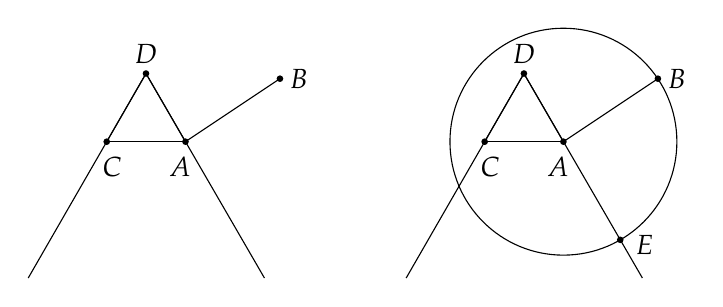
\begin{tikzpicture}[scale=0.4]
\begin{scope}
\coordinate (C) at (0,0);
\coordinate (A) at (2.5,0);
\coordinate (B) at (5.5,2);
\draw (A) node[below,xshift=-2pt,yshift=-2pt] {$A$} -- (B) node[right] {$B$};
\fill (A) circle[radius=3pt];
\fill (B) circle[radius=3pt];
\fill (C) node[below,xshift=2pt,yshift=-2pt] {$C$} circle[radius=3pt];
\draw (A) -- (C);
\path[name path=larc] (C) ++(-70:2.5cm) arc (-70:70:2.5cm);
\path[name path=rarc] (A) ++(-110:2.5cm) arc (-110:-250:2.5cm);
\path [name intersections={of=larc and rarc,by={d,D}}];
\fill (D) node[above] {$D$} circle[radius=3pt];
\draw (A) -- (D);
\draw (C) -- (D);
\draw[name path=ray2] (D) -- ($ (D) ! 3 ! (C) $);
\draw[name path=ray1] (D) -- ($ (D) ! 3 ! (A) $);
\end{scope}
\begin{scope}[xshift=12cm]
\coordinate (C) at (0,0);
\coordinate (A) at (2.5,0);
\coordinate (B) at (5.5,2);
\draw (A) node[below,xshift=-2pt,yshift=-2pt] {$A$} -- (B) node[right] {$B$};
\fill (A) circle[radius=3pt];
\fill (B) circle[radius=3pt];
\fill (C) node[below,xshift=2pt,yshift=-2pt] {$C$} circle[radius=3pt];
\draw (A) -- (C);
\path[name path=larc] (C) ++(-70:2.5cm) arc (-70:70:2.5cm);
\path[name path=rarc] (A) ++(-110:2.5cm) arc (-110:-250:2.5cm);
\path [name intersections={of=larc and rarc,by={d,D}}];
\fill (D) node[above] {$D$} circle[radius=3pt];
\draw (A) -- (D);
\draw (C) -- (D);
\draw[name path=ray2] (D) -- ($ (D) ! 3 ! (C) $);
\draw[name path=ray1] (D) -- ($ (D) ! 3 ! (A) $);
\node[draw,circle through=(B),name path=c1] at (A) {};
\path [name intersections={of=c1 and ray1,by={E,e}}];
\fill (E) node[right,xshift=2pt,yshift=-2pt] {$E$} circle[radius=3pt];
\end{scope}
\end{tikzpicture}
\end{center}


בנה מעגל שמרכזו 
$A$
עם רדיוס
$AB$.
$E$
הוא החיתוך של המעגל עם הקרן
$DE$
)תרשים מימין(.

בנה מעגל שמרכזו 
$D$
עם רדיוס 
$DC$.
סמן את החיתוך של הקרן
$DC$
עם המעגל ב-%
$F$:

\np

\begin{center}
\selectlanguage{english}
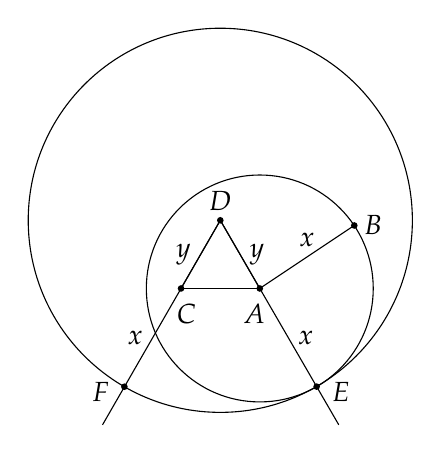
\begin{tikzpicture}[scale=0.4]
\coordinate (C) at (0,0);
\coordinate (A) at (2.5,0);
\coordinate (B) at (5.5,2);
\draw (A) node[below,xshift=-2pt,yshift=-2pt] {$A$} -- node[above] {$x$} (B) node[right] {$B$};
\fill (A) circle[radius=3pt];
\fill (B) circle[radius=3pt];
\fill (C) node[below,xshift=2pt,yshift=-2pt] {$C$} circle[radius=3pt];
\draw (A) -- (C);
\path[name path=larc] (C) ++(-70:2.5cm) arc (-70:70:2.5cm);
\path[name path=rarc] (A) ++(-110:2.5cm) arc (-110:-250:2.5cm);
\path [name intersections={of=larc and rarc,by={d,D}}];
\fill (D) node[above] {$D$} circle[radius=3pt];
\draw (A) -- node[right] {$y$} (D);
\draw (C) -- node[left] {$y$} (D);
\draw[name path=ray2] (D) -- ($ (D) ! 3 ! (C) $);
\draw[name path=ray1] (D) -- ($ (D) ! 3 ! (A) $);
\node[draw,circle through=(B),name path=c1] at (A) {};
\path [name intersections={of=c1 and ray1,by={E,e}}];
\fill (E) node[right,xshift=2pt,yshift=-2pt] {$E$} circle[radius=3pt];
\node[draw,circle through=(E),name path=c2] at (D) {};
\path [name intersections={of=c2 and ray2,by={F,f}}];
\fill (F) node[left,xshift=-2pt,yshift=-2pt] {$F$} circle[radius=3pt];
\path (A) -- node[right] {$x$} (E);
\path (C) -- node[left] {$x$} (F);
\end{tikzpicture}
\end{center}

\textbf{טענה:}
אורכו של קטע הקו
$CF$
שווה לאורך קטע הקו
$AB$.

%\vspace*{-7ex}
\textbf{הוכחה:}
$DC=DA$
כי
$\triangle ACD$
שווה צלעות.
$AE=AB$
כי שניהם רדיוסים של המעגל שמרכזו 
$A$.
$DF=DE$
כי שניהם רדיוסים של המעגל שמרכזו
$D$.
לכן, אורך קטע הקו 
$CF$ 
הוא:
\[
CF = DF - DC = DE - DC = DE - DA = AE = AB\,.
\].

%%%%%%%%%%%%%%%%%%%%%%%%%%%%%%%%%%%%%%%%%%%%%%%%%%%%%%%%%%%%%%%

\vspace{-8ex}

\section{%
העתקה שגויה של קטע קו
}\label{sec.error}

\hspace{-8pt}
\textbf{
משפט
\L{(Compasss Equivalency Theorem)}:
}
נתון קטע קו
$AB$
ונקודה
$C$,
ניתן לבנות )באמצעות מחוגה מתמוטטת( בנקודה
$C$
קטע קו שאורכו שווה לאורכו של 
$AB$.

\textbf{בנייה}
\L{(\cite{rusty})}:
%\vspace*{-2ex}

בנה מעגל שמרכזו 
$A$
עם רדיוס
$AB$:

\begin{center}
\selectlanguage{english}
\begin{tikzpicture}[scale=0.4]
\begin{scope}
\coordinate (C) at (-2,0);
\coordinate (A) at (2.5,0);
\coordinate (B) at (4.5,1.5);
\draw (A) node[below,xshift=-2pt,yshift=-2pt] {$A$} -- (B) node[right] {$B$};
\fill (A) circle[radius=3pt];
\fill (B) circle[radius=3pt];
\fill (C) node[below,xshift=2pt,yshift=-2pt] {$C$} circle[radius=3pt];
\end{scope}
\begin{scope}[xshift=12cm]
\coordinate (C) at (-2,0);
\coordinate (A) at (2.5,0);
\coordinate (B) at (4.5,1.5);
\draw (A) node[below,xshift=-2pt,yshift=-2pt] {$A$} -- (B) node[right] {$B$};
\fill (A) circle[radius=3pt];
\fill (B) circle[radius=3pt];
\fill (C) node[below,xshift=2pt,yshift=-2pt] {$C$} circle[radius=3pt];
\node[draw,circle through=(B),name path=c1] at (A) {};
\end{scope}
\end{tikzpicture}
\end{center}
%\vspace*{-8ex}

בנה מעגל שמרכזו
$A$
עם רדיוס
$AC$
ומעגל שמרכזו
$C$
עם רדיוס
$AC=CA$.
סמן את נקודות החיתוך של המעגלים ב-%
$E,F$,
וסמן את החיתוך של המעגל שמרכזו
$C$
עם המעגל שמרכזו
$A$
ב-%
$D$.

\begin{center}
\selectlanguage{english}
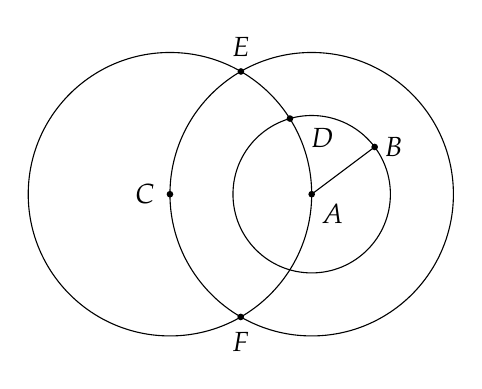
\begin{tikzpicture}[scale=0.4]
\coordinate (C) at (-2,0);
\coordinate (A) at (2.5,0);
\coordinate (B) at (4.5,1.5);
\draw (A) node[below right] {$A$} -- (B) node[right] {$B$};
\fill (A) circle[radius=3pt];
\fill (B) circle[radius=3pt];
\fill (C) node[left,xshift=-2pt] {$C$} circle[radius=3pt];
\node[draw,circle through=(B),name path=c1] at (A) {};
\node[draw,circle through=(C),name path=c2] at (A) {};
\node[draw,circle through=(A),name path=c3] at (C) {};
\path [name intersections={of=c1 and c3,by={D,f}}];
\path [name intersections={of=c2 and c3,by={E,F}}];
\fill (D) node[below right,xshift=4pt] {$D$} circle[radius=3pt];
\fill (E) node[above,yshift=2pt] {$E$} circle[radius=3pt];
\fill (F) node[below,yshift=-2pt] {$F$} circle[radius=3pt];
\end{tikzpicture}
\end{center}

בנה מעגל שמרכזו 
$E$
עם רדיוס 
$ED$.
סמן את החיתוך של מעגל זה עם המעגל שמרכזו
$C$
ב-%
$G$.
ארכו של קטע הקו 
$GC$
שווה לאורכו של
$AB$.

\np

\begin{center}
\selectlanguage{english}
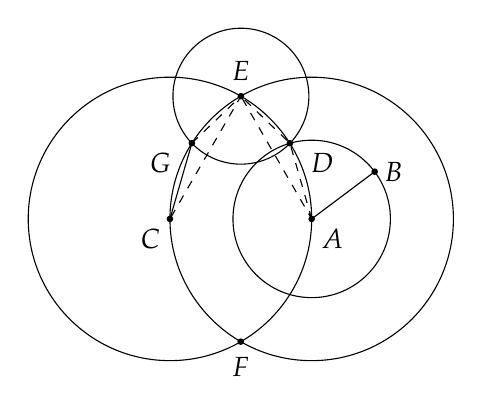
\begin{tikzpicture}[scale=0.4]
\coordinate (C) at (-2,0);
\coordinate (A) at (2.5,0);
\coordinate (B) at (4.5,1.5);
\draw (A) node[below right] {$A$} -- (B) node[right] {$B$};
\fill (A) circle[radius=3pt];
\fill (B) circle[radius=3pt];
\fill (C) node[below left] {$C$} circle[radius=3pt];
\node[draw,circle through=(B),name path=c1] at (A) {};
\node[draw,circle through=(C),name path=c2] at (A) {};
\node[draw,circle through=(A),name path=c3] at (C) {};
\path [name intersections={of=c1 and c3,by={D,f}}];
\path [name intersections={of=c2 and c3,by={E,F}}];
\fill (D) node[below right,xshift=4pt] {$D$} circle[radius=3pt];
\fill (E) node[above,yshift=2pt] {$E$} circle[radius=3pt];
\fill (F) node[below,yshift=-2pt] {$F$} circle[radius=3pt];
\node[draw,circle through=(D),name path=c4] at (E) {};
\path [name intersections={of=c2 and c4,by={g,G}}];
\fill (G) node[below left,xshift=-4pt] {$G$} circle[radius=3pt];
\draw (C) -- (G);
\draw[dashed] (G) -- (E) -- (C);
\draw[dashed] (A) -- (D) -- (E) -- cycle;
\end{tikzpicture}
\end{center}

חשוב להשתכנע שהבנייה אפשרית עם מחוגה מתמוטטת.

את ההוכחה ש-%
$AB=GC$
ניתן למצוא ב-%
\L{\cite{rusty}}.
בהוכחה יש להראות ששני המשולשים המסומנים בקווים במקוקווים חופפים כך ש-%
$GC=DA=AB$.
ההוכחה ארוכה הרבה יותר מההוכחה של אוקלידס ומשתמשת במושגים מתקדמים יחסית להוכחה של אוקלידס המשתמשת רק במושגים: כל הרדיוסים של מעגל שווים וכל הצלעות של משולש שווה צלעות שווים.

עברו בעיון על ההוכחה ב-%
\cite{rusty}
ש-%
$AB=GC$
וחפש את השגיאה. התשובה: אין שום שגיאה בהוכחה! השגיאה נובעת ממקור אחר: השווין
$AB=GC$
מתקיים רק כאשר אורכו של 
$AB$
קטן מאורכו של
$AC$.
הבנייה של אוקלידס נכונה ללא קשר לאורך היחסי של הקווים ולמיקום של הנקודה
$C$
ביחס לקטע הקו
$AB$
)\cite{toussaint}(.

%%%%%%%%%%%%%%%%%%%%%%%%%%%%%%%%%%%%%%%%%%%%%%%%%%%%%%%%%%%%%%%
\begin{comment}
\section{%
חקר הבניות עם גיאוגברה%
}
הכנתי קבצי גיאוגברה עבור שתי הבניות:
\begin{center}
\L{\texttt{compass-equivalency.ggb, rusty-compass.ggb}}.
\end{center}
ניתן להזיז את הנקודות
$A,B,C$
כדי לראות איך הציור משתנה, ולמדוד את שני אורכים כדי לבדוק אם הם שווים.

\textbf{%
שימו לב:%
}
בבנייה של אוקלידס, אם מתחילים עם 
$AB<AC$,
מזיזים את
$C$
כך ש-%
$AB>AC$
וחוזרים, התצוגה מתקלקלת. הסיבה היא שכאשר
$AB<AB$,
לקרן
$DA$
יש שתי נקודות חיתוך עם המעגל שמרכזו
$A$.
כאשר חוזרים למצב ש-%
$AB<AC$
נאבד נקודת החיתוך. כדי להתגבר על הבעייה הכנתי שני קבצים עבור שני מצבים.

\end{comment}
%%%%%%%%%%%%%%%%%%%%%%%%%%%%%%%%%%%%%%%%%%%%%%%%%%%%%%%%%%%%%%%

\section{
דרך "פשוטה יותר" להעתקת מעגל
}

נתון קטע קו 
$AB$
ונקודה
$C$,
אם נוכל לבנות מקבילית כאשר שלושת הנקודות הן קודקודים, נקבל קטע קו עם 
$C$
בקצה אחד שאורכו שווה לאורכו של
$AB$
)תרשים שמאלי(. ראו
\L{\cite[%
207--208
\R{עמ'}%
]{roads}}.

\begin{center}
\selectlanguage{english}
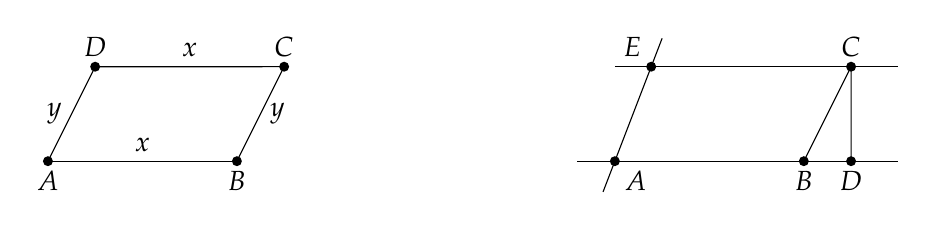
\begin{tikzpicture}[scale=0.6]
\coordinate (A) at (0,0);
\coordinate (B) at (4,0);
\coordinate (C) at (5,2);
\draw (A) -- (B);
\path (A) -- node[above] {$x$} (B);
\fill (A) node[below] {$A$} circle[radius=3pt];
\fill (B) node[below] {$B$} circle[radius=3pt];
\fill (C) node[above] {$C$} circle[radius=3pt];
\draw (B) -- node[right] {$y$} (C);
\coordinate (D) at ($(C)+(-40mm,0cm)$);
\draw (D) -- node[above] {$x$} (C);
\draw (A) -- node[left] {$y$} (D);
\fill (D) node[above] {$D$} circle[radius=3pt];
\begin{scope}[xshift=12cm]
\coordinate (A) at (0,0);
\coordinate (B) at (4,0);
\coordinate (C) at (5,2);
\draw ($ (B) ! 1.2 ! (A) $) -- ($ (A) ! 1.5 ! (B) $);
\path (A) -- (B);
\fill (A) node[below right] {$A$} circle[radius=3pt];
\fill (B) node[below] {$B$} circle[radius=3pt];
\fill (C) node[above] {$C$} circle[radius=3pt];
\draw (B) -- (C);
\draw[name path=ray1] ($(C)+(-5cm,0cm)$) -- ($(C)+(1cm,0cm)$);
\draw[name path=ray2] ($(A)+(-.25,-.65)$) -- ($(A)+(1,2.6)$);
\path [name intersections={of=ray1 and ray2,by={E}}];
\fill (E) node[above left] {$E$} circle[radius=3pt];
\coordinate (D) at (C |- B);
\draw (C) -- (D);
\fill (D) node[below] {$D$} circle[radius=3pt];
\end{scope}
\end{tikzpicture}
\end{center}

\textbf{בנייה} 
)תרשים מימין(:


חבר את
$B$
ו-%
$C$.

בנה אנך מ-%
$C$
לקו המכיל את הקטע
$AB$.
נסמן את נקודת החיתוך ב-%
$D$.

בנה אנך לקטע
$CD$
מהנקודה
$C$.
הקו המכיל את האנך מקביל ל-%
$AB$.

באותה דרך בנה קו המקביל ל-%
$BC$
דרך 
$A$. 
נסמן את נקודת החיתוך של שני הקווים ב-%
$E$.

אורכו של קטע הקו
$EC$
שווה לאורכו של
$AB$
ו-%
$C$
היא נקודת קצה שלו.


יש לוודא שאפשר לבנות את המקבילית עם מחוגה מתמוטטת. למעשה, הבנייה יחידה הנחוצה היא של אנך מנקודה שרירותית נתונה לקו המכיל קטע קו נתון:

\np

\begin{center}
\selectlanguage{english}
\begin{tikzpicture}[scale=0.5]
\coordinate (A) at (0,0);
\coordinate (B) at (4,0);
\coordinate (C) at (5,2);
\draw ($ (B) ! 1.5 ! (A) $) -- ($ (A) ! 1.5 ! (B) $);
\fill (A) node[below] {$A$} circle[radius=3pt];
\fill (B) node[below] {$B$} circle[radius=3pt];
\fill (C) node[right] {$C$} circle[radius=3pt];
\end{tikzpicture}
\end{center}

נבנה מעגל שמרכזו
$C$
עם רדיוס הגדול מהמרחק של
$C$
מהקו:
\begin{center}
\selectlanguage{english}
\begin{tikzpicture}[scale=0.5]
\coordinate (A) at (0,0);
\coordinate (B) at (4,0);
\coordinate (C) at (5,2);
\draw[name path=ray] ($ (B) ! 1.5 ! (A) $) -- ($ (A) ! 2.5 ! (B) $);
\fill (A) node[below] {$A$} circle[radius=3pt];
\fill (B) node[below] {$B$} circle[radius=3pt];
\fill (C) node[right] {$C$} circle[radius=3pt];
\draw[name path=arc] (C) ++(-160:3.5cm) arc (-160:-20:3.5cm);
\path [name intersections={of=arc and ray,by={D,E}}];
\fill (D) node[below left] {$D$} circle[radius=3pt];
\fill (E) node[below right] {$E$} circle[radius=3pt];
\end{tikzpicture}
\end{center}


בנה אנך אמצעי ל-%
$DE$
דרך 
$C$.
$CD=CE$
כי הם שני רדיוסים שווים של אותו מעגל וניתן לבנות את האנך באמצעות מחוגה מתמוטטת:

\begin{center}
\selectlanguage{english}
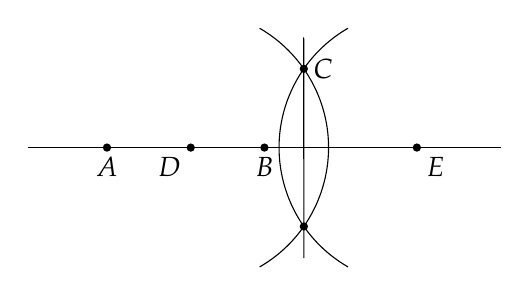
\begin{tikzpicture}[scale=0.5]
\coordinate (A) at (0,0);
\coordinate (B) at (4,0);
\coordinate (C) at (5,2);
\draw[name path=ray] ($ (B) ! 1.5 ! (A) $) -- ($ (A) ! 2.5 ! (B) $);
\fill (A) node[below] {$A$} circle[radius=3pt];
\fill (B) node[below] {$B$} circle[radius=3pt];
\fill (C) node[right] {$C$} circle[radius=3pt];
\path[name path=arc] (C) ++(-160:3.5cm) arc (-160:-20:3.5cm);
\path [name intersections={of=arc and ray,by={D,E}}];
\fill (D) node[below left] {$D$} circle[radius=3pt];
\fill (E) node[below right] {$E$} circle[radius=3pt];
\draw[name path=larc] (D) ++(-60:3.5cm) arc (-60:60:3.5cm);
\draw[name path=rarc] (E) ++(-120:3.5cm) arc (-120:-240:3.5cm);
\path [name intersections={of=larc and rarc,by={b,t}}];
\fill (b) circle[radius=3pt];
\draw ($ (b) ! 1.2 ! (t)$) -- ($ (t) ! 1.2 ! (b)$);
\end{tikzpicture}
\end{center}

למה אוקלידס לא הביא בנייה זו? כפי שהזכרנו לעיל, הוכחת הנכונות של הבנייה של אנך אמצעי כלל לא פשוטה, בעוד הוכחת הנכונות של הבנייה של אוקלידס מסתמכת על משפט פשוט אחד.


%%%%%%%%%%%%%%%%%%%%%%%%%%%%%%%%%%%%%%%%%%%%%%%%%%%%%%%%%%%%%%%

\begin{comment}

\section{
הגבלות והרחבות של בנייה באמצעות סרגל ומחוגה
}

ראינו שמה שניתן לבנות עם סרגל ומחוגה קבועה ניתן לבנות עם סרגל ומחוגה מתקפלת. מתמטיקאים חקרו אפשרות מוגבלות יותר:

\begin{itemize}
\item
כל בנייה עם סרגל ומחוגה ניתנת לבנייה עם מחוגה בלבד! כמובן, אם אין סרגל לא נראה קווים, אבל שתי נקודות במישור מגדירות קו ואין צורך ממש לראות אותו. למשל, אם ניתנות שתי נקודות
$A,B$
אפשר לבנות עם מחוגה בלבד נקודה
$C$
שהמרחק שלה מ-%
$A$
ומ-%
$B$
שווה למרחק
$AB$
)איור~%
\ref{fig.mm}(.
בנינו משולש שווה צלעות, אמנם ללא צלעות. המשפט הוכח בשנת
\L{1672}
על ידי
\L{Georg Mohr}
ובאופן עצמאי בשנת
\L{1797}
על ידי
\L{Lorenzo Mascheroni}.
\begin{figure}[H]
\begin{center}
\selectlanguage{english}
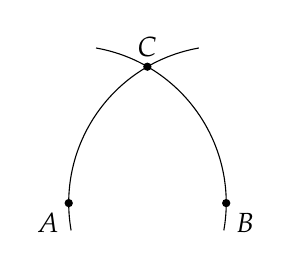
\begin{tikzpicture}[scale=0.5]
\coordinate (A) at (0,0);
\coordinate (B) at (4,0);
\path (A) node[below left] {$A$} -- (B) node[below right] {$B$};
\fill (A) circle[radius=3pt];
\fill (B) circle[radius=3pt];
\draw[name path=larc] (A) ++(-10:4cm) arc (-10:80:4cm);
\draw[name path=rarc] (B) ++(-170:4cm) arc (-170:-260:4cm);
\path [name intersections={of=larc and rarc,by={t}}];
\fill (t) node[above] {$C$} circle[radius=3pt];
\end{tikzpicture}
\selectlanguage{hebrew}
\caption{%
בניית משלוש שווה צלעות עם מחוגה בלבד.%
}\label{fig.mm}
\end{center}
\end{figure}
\vspace*{-8ex}
\item
אי-אפשר להסתפק בסרגל בלבד, אבל אם קיים במישור מעגל אחד בלבד )לא משנה איפה מרכז המעגל או הרדיוס שלו(, ניתן לבנות את כל מה שאפשר לבנות עם סרגל ומחוגה. המשפט הוכח ב-%
\L{1833}
על ידי 
\L{Jacob Steiner}.
\end{itemize}
ההוכחות של שני המשפטים מעט ארוכות אבל לא מסובכות במיוחד. אפשר למצוא אותן בספרו של
\L{Heinrich D\"{o}rrie}
\L{\cite{dorrie1}}.
ספר זה נגיש יותר במהדורה חדשה 
\L{\cite{dorrie2}}.

בכיוון השני, היוונים חקרו מה אפשר לבנות אם משתמשים בכלים מורכבים יותר מסרגל )ללא סימנים( ומחוגה. במאה ה-%
\L{19}
הוכח שלא ניתן לחלק זווית לשלושה חלקים שווים באמצעות סרגל ומחוגה. ניתן לבצע את הבנייה עם סרגל בעל שני סימנים הנקרא
\L{neusis}
או עם מכשיר הנקרא
\L{quadratrix},
המורכב משני סרגלים המחוברים כך שהם יכולים לגלוש אחד ליד השני ולהסתובב. כתבתי מסמך המתאר את הבניות
\textbf{איך לחלק זווית לשלושה )אם אתם מוכנים לרמות(}
שניתן למצוא באתר שלי:\\
\selectlanguage{english}
\url{http://www.weizmann.ac.il/sciÎtea/benari/mathematics}.

\end{comment}
%%%%%%%%%%%%%%%%%%%%%%%%%%%%%%%%%%%%%%%%%%%%%%%%%%%%%%%%%%%%%%%

\selectlanguage{hebrew}

\section{
אין לסמוך על ציור
}
בסעיף~%
\ref{sec.error}
ראינו שאין לסמוך על ציור. הנה הוכחה "נכונה"
\textbf{\R{שכל}}
משולש שווה שוקיים!

נתון משולש שרירותי 
$ABC$,
תהי
$P$
נקודת החיתוך בין חוצה הזווית של
$\angle BAC$
לבין האנך האמצעי של 
$BC$.
סימנו ב-%
$D,E,F$
את נקודות החיתוך של האנחים מ-%
$P$
לצלעות
$BC,AB,AC$. $\triangle APE\cong \triangle APF$
כי הם משולשים ישר זווית עם זוויות שוות
$\alpha$
וצלע $AP$ משותף.

$\triangle DPB\cong \triangle DPC$
לפי צ.ז.צ. כי 
$PD$
הוא צלע משותף, ו-%
$BD=DC=a$
כי 
$PD$
הוא האנך האמצעי ל-%
$BC$.
$\triangle EPB\cong \triangle FPC$,
כי
$EP=PF$
לפי החפיפה הראשונה, ו-%
$PB=PC$
לפי החפיפה השנייה. נחבר את השוויונות ונקבל ש-%
$\triangle ABC$
שווה שוקיים:
\[
AB=AE+EB=AF+FC=AC\,.
\]

\np

\begin{center}
\selectlanguage{english}
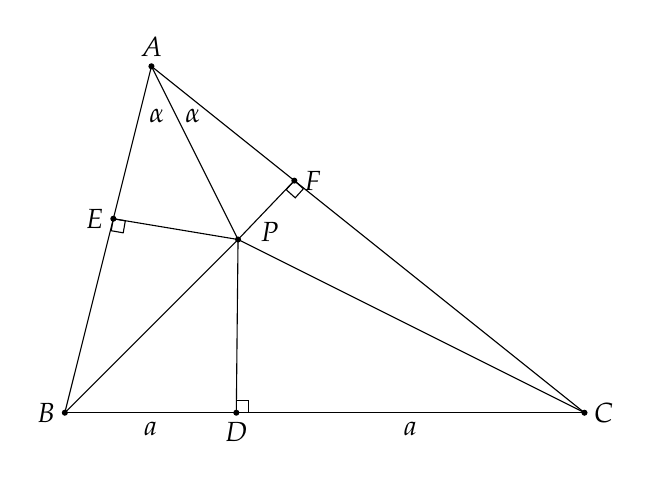
\begin{tikzpicture}[scale=1.1]
\coordinate (P) at (0,0);
\node[xshift=4mm,yshift=1mm] at (P) {$P$};
\coordinate [label=left:$B$] (B)  at (-2,-2);
\coordinate [label=right:$C$] (C)  at (4,-2);
\coordinate [label=above:$A$] (A)  at (-1,2);
\node[below,yshift=-12pt,xshift=2pt] at (A) {$\alpha$};
\node[below,yshift=-12pt,xshift=15pt] at (A) {$\alpha$};
\draw (A) -- (B);
\draw (A) -- (C);
\draw (B) -- (C);
\draw (A) -- (P);
\draw (B) -- (P);
\draw (C) -- (P);
\coordinate[label=left:$E$] (E) at ($ (A) ! .44 ! (B) $);
\draw[rotate=-100] (E) rectangle +(4pt,4pt);
\draw (P) -- (E);
\coordinate[label=right:$F$] (F) at ($ (A) ! .33 ! (C) $);
\draw[rotate=-132] (F) rectangle +(4pt,4pt);
\draw (P) -- (F);
\coordinate[label=below:$D$] (D) at ($ (B) ! .33 ! (C) $);
\draw (D) rectangle +(4pt,4pt);
\draw (P) -- (D);
\node[left] at ($ (A) ! .5 ! (E) $) {};
\node[left] at ($ (B) ! .5 ! (E) $) {};
\node[below] at ($ (B) ! .5 ! (D) $) {$a$};
\node[below] at ($ (C) ! .5 ! (D) $) {$a$};
\node[right,xshift=2pt] at ($ (A) ! .5 ! (F) $) {};
\node[right,xshift=2pt] at ($ (C) ! .5 ! (F) $) {};
\fill (A) circle(1pt);
\fill (B) circle(1pt);
\fill (C) circle(1pt);
\fill (D) circle(1pt);
\fill (E) circle(1pt);
\fill (F) circle(1pt);
\fill (P) circle(1pt);
\end{tikzpicture}
\end{center}
הבעיה בהוכחה היא שהאיור אינו נכון כי הנקודה
$P$
נמצאות
\textbf{\R{מחוץ}}
למשולש:

\medskip

\begin{center}
\selectlanguage{english}
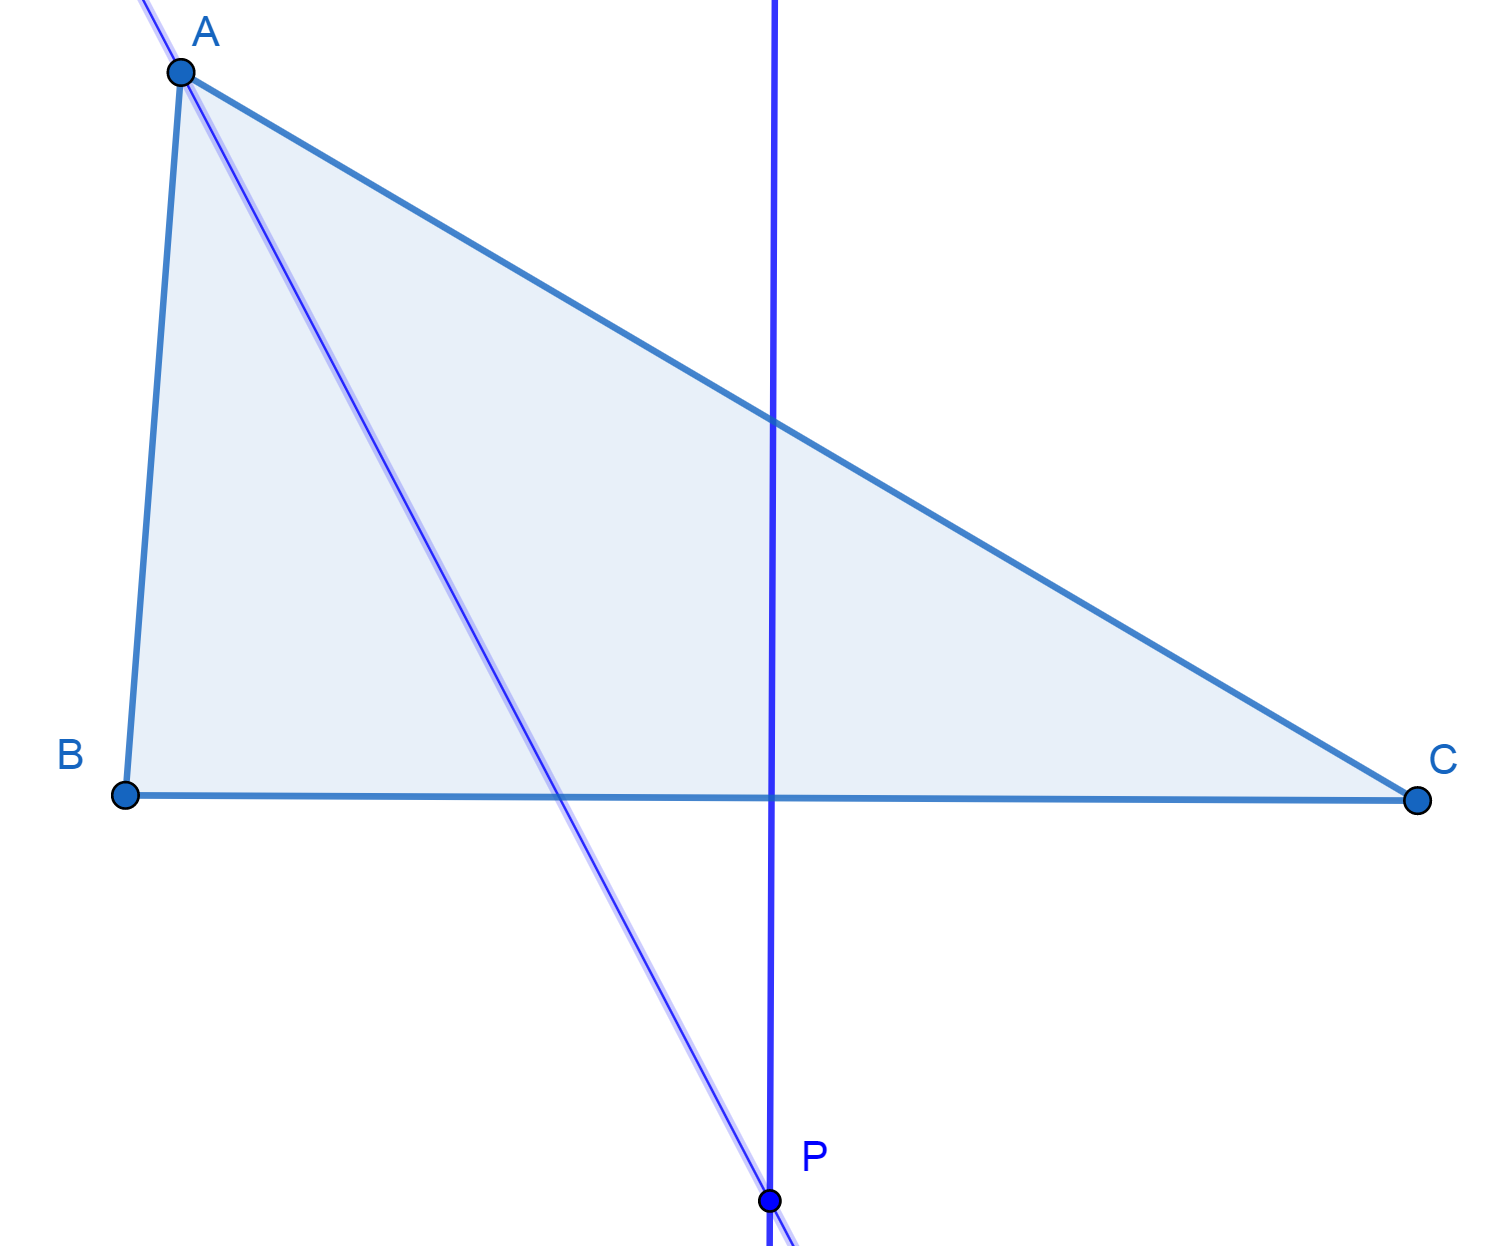
\includegraphics[width=.5\textwidth]{isoceles}
\end{center}

\selectlanguage{english}

%%%%%%%%%%%%%%%%%%%%%%%%%%%%%%%%%%%%%%%%%%%%%%%%%%%%%%%%%%%%%%%


\tikzsetfigurename{trisect-an-angle}
% !TeX root = construct.tex

\selectlanguage{hebrew}
\chapter[\R{ איך לחלק זווית לשלושה )אם אתם מוכנים לרמות( }]%
{איך לחלק זווית לשלושה\\)אם אתם מוכנים לרמות(}
\label{c.trisect-an-angle}

%%%%%%%%%%%%%%%%%%%%%%%%%%%%%%%%%%%%%%%%%%%%%%%%%%%%%%%%%%%%%

ידוע שלא ניתן לחלק זווית שרירותית לשלושה בעזרת מחוגה וסרגל. הסיבה היא שחלוקת זווית לשלושה דורשת בנייה של שורש שלישי, אבל עם מחוגה וסרגל ניתן לבנות רק אורכים המתקבלים מארבעת פעולות החשבון וכן שורש ריבועי.

המתמטיקאים היוונים גילו שבאמצעות כלים אחרים ניתן לחלק זווית לשלושה. סעיף~%
\L{\ref{s.neusis}}
מציג בנייה של ארכימדס עם כלי פשוט הנקרא ביוונית ניאוסיס
\L{(neusis)}.
סעיף~%
\L{\ref{s.q}}
מביא בנייה מסובכת יותר של היפיאס באמצעות
\qd{}
\L{(quadratrix)}.
כהטבה מיוחדת, נראה בסעיף~%
\L{\ref{s.square}}
איך ניתן לרבע מעגל באמצעות 
\qd{}.


מקורות:

\selectlanguage{english}
\noindent\url{https://en.wikipedia.org/wiki/Angle_trisection}\\
\url{https://en.wikipedia.org/wiki/Quadratrix_of_Hippias}\\
\url{https://en.wikipedia.org/wiki/Neusis_construction}
\selectlanguage{hebrew}

\vspace{-2ex}

%%%%%%%%%%%%%%%%%%%%%%%%%%%%%%%%%%%%%%%%%%%%%%%%%%%%%%%%%%%%%

\section{חלוקת זווית לשלושה באמצעות ניאוסיס}\label{s.neusis}

לבניית צורות באמצעות סרגל ומחוגה מקום מרכזי בגיאומטריה. השימוש במילה "סרגל" מטעה, כי הכוונה היא למקל ישר ללא כל סימן, שהפעולה היחידה שניתן לעשות איתו היא למתוח קו ישר בין שתי נקודות. לסרגל המוכר יש סימנים המאפשרים למדוד אורכים. כדי לחלק זווית לשלושה, נשתמש ב-%
\textbf{ניאוסיס}
שהוא מקל עם שני סימנים בלבד. נניח שהמרחק בין שני הסימנים הוא
$1$:
\begin{center}
\selectlanguage{english}
\begin{tikzpicture}[scale=3.5]
\draw (-1,1.05) rectangle +(3.2,.1);
\draw[thick] (1.89,1.05) -- +(0,.1);
\draw[thick] (.73,1.05) -- +(0,.1);
\draw[<->] (.73,1.25) -- node[fill=white] {$1$} (1.89,1.25);
\end{tikzpicture}
\end{center}
תהי 
$\alpha$
זווית שרירותית
$\angle ABE$
בתוך מעגל שמרכזו
$B$
עם רדיוס
$1$.
ניתן לבנות את המעגל על ידי קביעת המרחק בין רגלי החוגה למרחק בין סימני הניאוסיס. בנה קרן כהמשכו של 
$EB$
מחוץ למעגל. הנח את הניאוסיס על הנקודה
$A$
והזז אותו עד שהוא חותך את הקרן בנקודה 
$D$
ואת המעגל בנקודה
$C$.
כוון את הניאוסיס כך שהאורך של
$CD$
יהיה
$1$.
צייר את הקו
$AD$:


\begin{center}
\selectlanguage{english}
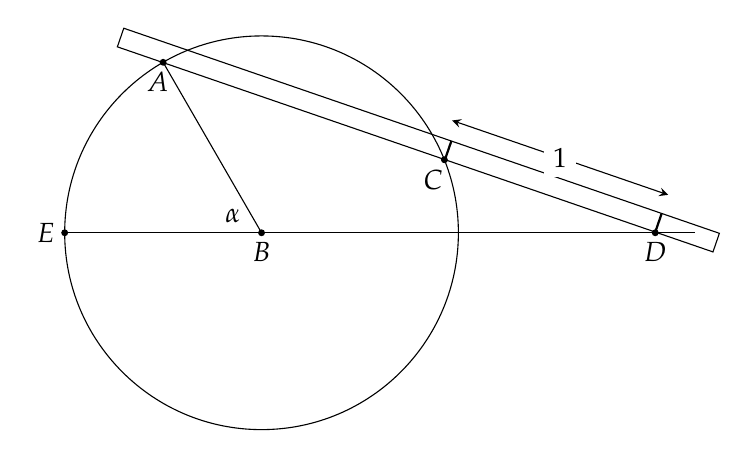
\begin{tikzpicture}[scale=2.5]
\coordinate (origin) at (0,0) node[below] {$B$} ;
\draw[name path=circle] (origin) circle [radius=1];
\draw (origin) node[above left,xshift=-4pt] {$\alpha$} -- (120:1) coordinate (a) node[below,xshift=-2pt] {$A$} ;
\draw (-1,0) -- (2.2,0);
\path[name path=ad] (a) -- (0,0 -| 2,0) coordinate (d) node[below] {$D$} ;
\path[name intersections={of=circle and ad,by={c,a1}}];
\fill (origin) circle [radius=.5pt];
\fill (a) circle [radius=.5pt];
\fill (c) circle [radius=.5pt] node [below,xshift=-4pt] {$C$};
\fill (d) circle [radius=.5pt];
\fill (-1,0) circle [radius=.5pt] node [left] {$E$};
\begin{scope}[rotate=-19,yshift=-11.25pt]
\draw (-1,1.05) rectangle +(3.2,.1);
\draw[thick] (1.89,1.05) -- +(0,.1);
\draw[thick] (.76,1.05) -- +(0,.1);
\draw[<->] (.73,1.25) -- node[fill=white] {$1$} (1.89,1.25);
\end{scope}
\end{tikzpicture}
\end{center}

\np

צייר את הקו 
$BC$
וסמן את הזוויות וקטעי הקו בתרשים:
\begin{center}
\selectlanguage{english}
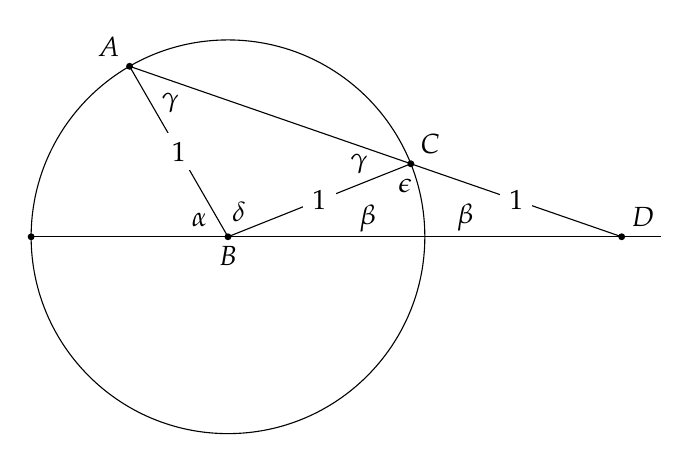
\begin{tikzpicture}[scale=2.5]
\coordinate (origin) at (0,0) node[below] {$B$} ;
\draw[name path=circle] (origin) circle [radius=1];
\draw (origin) node[above left,xshift=-4pt] {$\alpha$} node[above,xshift=4pt,yshift=2pt] {$\delta$} node[above right,xshift=44pt,yshift=-2pt] {$\beta$} -- node[fill=white] {$1$} (120:1) coordinate (a) node[above left] {$A$} ;
\draw (-1,0) -- (2.2,0);
\draw[name path=ad] (a) node[below right,xshift=8pt,yshift=-6pt] {$\gamma$} -- (0,0 -| 2,0) coordinate (d) node[left,xshift=-50pt,yshift=7pt] {$\beta$} node[above right] {$D$} ;
\path[name intersections={of=circle and ad,by={c,a1}}];
\draw (origin) -- node[fill=white] {$1$}(c) node[above right] {$C$} node[left,xshift=-12pt] {$\gamma$} node[below,xshift=-2pt,yshift=-2pt] {$\epsilon$};
\fill (origin) circle [radius=.5pt];
\fill (a) circle [radius=.5pt];
\fill (d) circle [radius=.5pt];
\fill (c) circle [radius=.5pt];
\fill (-1,0) circle [radius=.5pt];
\path (c) -- node[fill=white] {$1$} (d);
\end{tikzpicture}
\end{center}

$BA=BC$
כי שניהם רדיוסים ו-%
$CB=CD$
לפי הבניה באמצעות הניאוסיס. לכן 
$\triangle ABC$, $\triangle BCD$
שווי שוקיים. החישוב שלהלן משתמש בעובדות שסכום הזוויות של משולש ושל זוויות משלימות הוא
$180$:

\vspace{-3ex}

\erh{2pt}
\begin{equationarray*}{rcl}
\epsilon &=& 180 - 2\beta\\
\gamma &=& 180 - \epsilon = 2\beta\\
\delta &=& 180 - 2\gamma = 180 - 4\beta\\
\alpha &=& 180 - \delta - \beta = 4\beta -\beta =3\beta\,.
\end{equationarray*}
\vspace{-2ex}
הזווית
$\beta$
היא שליש הזווית
$\alpha$.
%%%%%%%%%%%%%%%%%%%%%%%%%%%%%%%%%%%%%%%%%%%%%%%%%%%%%%%%%%%%%


\section{חלוקת זווית לשלושה באמצעות
\qd{}%
}\label{s.q}

התרשים שלהלן מראה
\textbf{מחוגת \qd{}}
המורכב משני סרגלים )ללא סימנים( המחוברים במפרק המאלץ אותם לנוע ביחד. סרגל אחד נע במקביל לציר ה-%
$x$
מ-%
$DC$
עד
$AB$.
הסרגל השני מחובר לנקודה
$A$
ומסתובב ממצב אנכי לאורך 
$AD$
עד שהוא במצב אופקי לאורך 
$AB$. 
העקומה המצוירת על ידי המפרק המחבר את שני הסרגלים נקראת
\textbf{עקומת ה%
\qd{}%
}
או פשוט
\textbf{\qd{}}.
\begin{center}
\selectlanguage{english}
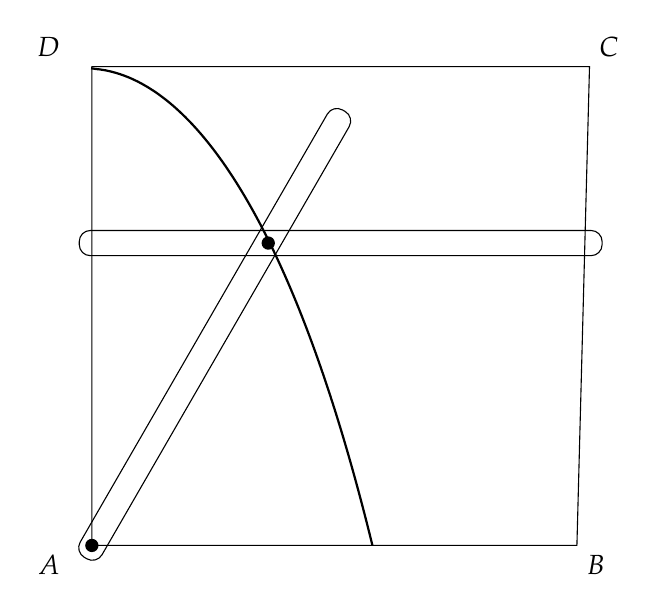
\begin{tikzpicture}[scale=.8,domain=.03:1.555,samples=100]
\draw (.1,.2) node[below left,xshift=-8pt] {$A$} -- (7.8,.2) node[below right] {$B$} -- (8,7.8) node[above right] {$C$} -- (.1,7.8) node[above left,xshift=-8pt] {$D$} -- cycle;
%\draw (.1,7.8) -- (.1,.2) -- (8,.1) -- (8,7.8);
\draw[rounded corners,rotate=60] (0,-.2) rectangle (8.2,.2);
\draw[rounded corners] (-.1,4.8) rectangle (8.2,5.2);
\fill (2.9,5) circle [radius=3pt];
\fill (.1,.2) circle [radius=3pt];
\draw[thick] plot (4.6*.637*\x,{12.2*.637*\x*cot(\x r)});
\end{tikzpicture}
\end{center}

\np

כאשר מזיזים את הסרגל האופקי במהירות אחידה, החיבור מאלץ את הסרגל השני להסתובב במהירות זוותית קבועה. למעשה זו ההגדרה של ה%
\qd{}.
כאשר קואורדינטת ה-%
$y$
של הסרגל האופקי יורד מ-%
$1$
ל-%
$0$,
הזווית של הסרגל השני יחסית לציר ה-%
$x$
יורד מ-%
$90^\circ$
ל-%
$0^\circ$.
התרשים שלהלן מראה איך אפשר לחלוק זווית שרירותית 
$\alpha$
לשלושה באמצעות
\qd{}:

\vspace{-2ex}

\begin{center}
\selectlanguage{english}
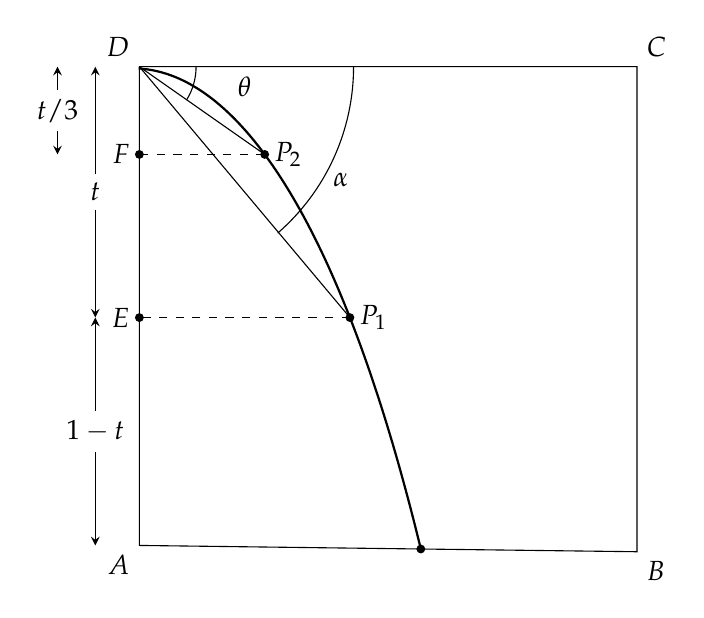
\begin{tikzpicture}[scale=.8,domain=.03:1.562,samples=100]
\draw (.1,7.8) coordinate (start) node[above left] {$D$} node[below right,xshift=32pt] {$\theta$} -- (.1,.2) node[below left] {$A$} -- (8,.1) node[below right] {$B$} -- (8,7.8) node[above right] {$C$} -- cycle;
\draw[name path=curve,thick] plot (4.6*.637*\x,{12.2*.637*\x*cot(\x r)});
\path[name path=twenty] (start) -- +(-35:9);
\path[name path=sixty] (start) -- +(-50:9);
\path[name path=xaxis] (.1,.2) -- (8,.1);
\path[name intersections={of=twenty and curve,by={x1,tri}}];
\draw (start) -- (tri);
\fill (tri) circle [radius=2pt] node[right] {$P_2$};
\path[name intersections={of=sixty and curve,by={x2,angle}}];
\fill (angle) circle [radius=2pt] node[right] {$P_1$};
\draw (start) -- (angle);
\path[name intersections={of=xaxis and curve,by=x}];
\fill (x) circle [radius=2pt];
%\path (.1,.2) -- node[below] {$2/\pi$} (x);
\draw[dashed] (tri) -- (tri -| .1,.2) coordinate (t3);
\fill (t3) circle [radius=2pt] node[left] {$F$};
\draw[dashed] (angle) -- (angle -| .1,.2) coordinate (t);
\fill (t) circle [radius=2pt] node[left] {$E$};
\draw[<->] (-1.2,7.8) -- node[fill=white] {$t/3$} (-1.2,7.8 |- t3);
\draw[<->] (-.6,7.8) -- node[fill=white] {$t$} (-.6,7.8 |- t);
\draw[<->] (-.6,7.8 |- t) -- node[fill=white] {$1-t$} (-.6,.2);
\draw (3.5,7.8) arc[start angle=0,delta angle=-49,radius=3.5];
\draw (1,7.8) arc[start angle=0,delta angle=-32,radius=1];
\node at (3.3,6) {$\alpha$}; 
\end{tikzpicture}
\end{center}

\vspace{-3ex}

הנקודה
$P_1$
היא החיתוך בין הקו המגדיר את הזווית 
$\alpha$
לבין ה%
\qd{}.
קואורדינטת ה-%
$y$
שלה היא
$1-t$,
כאשר 
$t$
הוא המרחק שהסרגל האופקי נע ממקומו ההתחלתי
$DC$.
חלק את
$DE$
לשלושה חלקים כדי לקבל את הנקודה
$F$
)קל לחלק
\textbf{קטע הקו}
לחלקים שווים על ידי שימוש במשפט תאלס(. הנקודה
$P_2$
היא נקודת החיתוך בין הקו מ-%
$F$
המקביל ל-%
$DC$
לבין ה%
\qd{}.
לפי העיקרון של מהירויות שוות:

\vspace{-4ex}

\erh{12pt}
\begin{equationarray*}{rcl}
\frac{\theta}{\alpha} &=& \frac{t/3}{t}\\
\theta &=& \alpha/3\,.
\end{equationarray*}

\vspace{-8ex}

%%%%%%%%%%%%%%%%%%%%%%%%%%%%%%%%%%%%%%%%%%%%%%%%%%%%%%%%%%%%%

\section{ריבוע המעגל באמצעות
\qd{}%
}\label{s.square}


\begin{center}
\selectlanguage{english}
\begin{tikzpicture}[scale=.8,domain=.01:1.57,samples=100]
\draw (0,0) node[below left] {$A$} node [above right,xshift=10pt] {$\theta$} -- (8,0) node[below right] {$B$} -- (8,8) node[above right] {$C$} -- (0,8) node[above left] {$D$} -- cycle;
\draw[name path=horiz] (0,5) -- (8,5);
\draw[name path=slant] (0,0) -- (61:8);
\path[name intersections={of=horiz and slant,by=joint}];
\draw[dashed] (joint) -- node[right] {$y$} (joint |- 0,0) coordinate (f);
\path (0,0) -- node[below] {$x$} (0,0 -| joint) node[below] {$F$};
\path (0,5) node[left] {$E$} -- node[left] {$t$} (0,8);
\path (0,0) -- node[left] {$1-t$} (0,5);
\fill (joint) circle [radius=2pt] node[above right,xshift=4pt] {$P$};
\fill (f) circle [radius=2pt];
\fill (0,5) circle [radius=2pt];
\fill (4.28,0) circle [radius=2pt] node[below] {$G$};
\draw[name path=curve,thick] plot (4.3*.637*\x,{12.5*.637*\x*cot(\x r)});
\end{tikzpicture}
\end{center}

\np

נניח שהסרגל האופקי נע מרחק 
$t$
לאורך ציר ה-%
$y$
עד לנקודה
$E$,
והסרגל המסתובב מגדיר זווית 
$\theta$
עם ציר ה-%
$x$.
הנקודה 
$P$
היא החיתוך בין
\qd{}
לבין הסרגל האופקי, והנקודה
$F$
היא היטל של 
$P$
על ציר ה-%
$x$.
מהן הקואורדינטות של הנקודה 
$P$
על ה%
\qd{}?
ברור ש:
\[
y=PF=EA=1-t\,.
\]
על העקומה,
$\theta$
יורד באותו קצב ש-%
$t$
עולה:
\erh{12pt}
\begin{equationarray*}{rcl}
\frac{1-t}{1} &=& \frac{\theta}{\pi/2}\\
\theta &=&\frac{\pi}{2}(1-t)\,.
\end{equationarray*}
נבדוק אם זה הגיוני: כאשר
$t=0$
אז
$\theta=\pi/2$,
וכאשר
$t=1$
אז
$\theta=0$.

את קואורדינטת ה-%
$x$
של
$P$
נקבל בטריגונומטריה:
\[
\tan \theta = \frac{y}{x}\,.
\]
ומכאן:

\[
x = \frac{y}{\tan\theta}=y\cot\theta=y\cot \frac{\pi}{2}(1-t)=y\cot \frac{\pi}{2}y\,.
\]

בדרך כלל המשוואה של עקומה היא מהצורה
$y=f(x)$,
אבל אפשר גם להשתמש במשוואה מהצורה
$x=f(y)$.
נחשב את קוארדינטת ה-%
$x$
של הנקודה 
$G$,
החיתוך של ה%
\qd{}
עם ציר ה-%
$x$.
לא ניתן להציב
$y=0$
כי
$\cot 0$
לא מוגדר, אבל ייתכן שיהיה לנו מזל אם נחשב את הגבול של
$x$
כאשר 
$y$
שואף ל-%
$0$:

\[
x = y\cot \frac{\pi}{2}y = \frac{2}{\pi}\cdot \frac{\pi}{2}y\cot \frac{\pi}{2}y\,.
\]

למען הנוחיות, נחליף משתנה
$z=\disfrac{\pi}{2}y$,
ואז נחשב את הגבול:

\[
\lim_{z\rightarrow 0} z\cot z = \lim_{z\rightarrow 0} \frac{z\cos z}{\sin z} = \lim_{z\rightarrow 0} \frac{\cos z}{\disfrac{\sin z}{z}} = \frac{\cos 0}{1} = 1\,,
\]

השתמשנו בעובדה הידועה ש-%
$\lim_{z\rightarrow 0} \disfrac{\sin z}{z}=1$.

כאשר
$y\rightarrow 0$:

\[
x \rightarrow \frac{2}{\pi}\cdot \lim_{y\rightarrow 0}\frac{\pi}{2}y\cot \frac{\pi}{2}y = \frac{2}{\pi}\cdot 1 = \frac{2}{\pi}\,.
\]

על ידי שימוש ב%
\qd{}
בנינו קטע קו
$AG$
שאורכו
$x=\disfrac{2}{\pi}$.
עם סרגל רגיל ומחוגה, קל לבנות קו באורך
$\sqrt{\pi}=\sqrt{\disfrac{2}{x}}$,
ואז לבנות ריבוע ששטחו
$\pi$.

\selectlanguage{english}


\tikzsetfigurename{square-a-circle}
% !TeX root = construct.tex

\selectlanguage{hebrew}
\chapter{%
איך לרבע את המעגל )בערך(}

\section{
קירובים ל-%
$\pi$}\label{s.square-intro}

במאה התשע-עשרה הוכח שאין בניות עם סרגל ומחוגה לשלוש בעיות: חלוקת זווית לשלושה חלקים שווים, הכפלת קוביה וריבוע מעגל. נתון קטע קו שאורכו מוגדר כ-%
$1$,
הערכים )אורכים( שניתנים לבנייה הם אלה שמתקבלים מקטע זו ומהפעולות 
$+,-,\times,/,\surd$.

בבניות בפרק זה נצטרך לחלק קטע קו לשלושה חלקים; כאן נראה איך לבנות קו שאורכו הוא החילוק של האורכים של שני קטעי קו נתונים. נתון קטע קו באורך 
$1$
וקטעי קו באורכים 
$a,b$,
לפי משולשים דומים
$1/b=\overline{OD}/a$
ולכן
$\overline{OD}=a/b$.

\begin{center}
\selectlanguage{english}
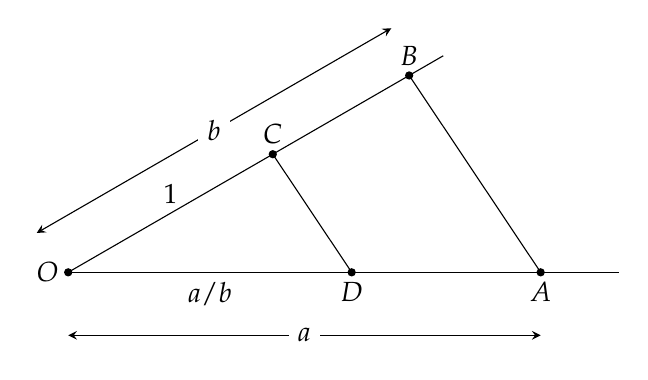
\begin{tikzpicture}
%\clip (-.6,-1) rectangle (4,3);
\draw[name path=horz] (0,0) coordinate (o) -- (7,0);
\fill (o) circle(1.5pt) node[left] {$O$};
\fill (6,0) circle(1.5pt) coordinate (a) node[below] {$A$};
\draw (0,0) -- (30:5.5);
\fill (30:3) circle(1.5pt) coordinate (c) node[above] {$C$};
\fill (30:5) circle(1.5pt) coordinate (b) node[above] {$B$};
\draw (a) -- (b);
\path[name path=par] (c) -- +($(a)-(b)$);
\path[name intersections={of=par and horz,by=d}];
\fill (d) circle(1.5pt) node[below] {$D$};
\draw (c) -- (d);
\draw[<->] (-.4,.5) -- node[fill=white] {$b$} +(30:5.2);
\path (o) -- node[above] {$1$} (c);
\draw[<->] (0,-.8) -- node[fill=white] {$a$} +(6,0);
\path (o) -- node[below] {$a/b$} (d);
\end{tikzpicture}
\end{center}

כדי לרבע מעגל יש לבנות את האורך 
$\sqrt{\pi}$,
אבל
$\pi$
הוא טרנסנדנטי, כלומר, הוא אינו פתרון של אף משוואה אלגברית.

פרק זה מביא שלוש בניות של קירובים ל-%
$\pi$.
הטבלה שלהלן מביא את הנוסחאות של האורכים שנבנים, קירוב לערכן, ההפרש בין ערכים אלה והערך של 
$\pi$,
והשגיאה במטרים אם משתמשים בקירוב כדי לחשב את היקף כדור הארץ כאשר נתון שהרדיוס הוא
$6378$
ק"מ.
\[
\selectlanguage{english}
\renewcommand{\arraystretch}{1.2}
\begin{array}{|l|c|c|c|c|}
\hline
\textrm{\R{הבנייה}} & \textrm{\R{הנוסחה}} &\textrm{\R{הערך}} & \textrm{\R{ההפרש}} & \textrm{\R{השגיאה )מ(}}\\\hline
\pi & & 3.14159265359 & - & -\\\hline
\textrm{Kochansky} & \sqrt{\disfrac{40}{3}-2\sqrt{3}}&
  3.14153338705 & 5.932 \times 10^{-5} & 756\\\hline
\textrm{Ramanujan}\; 1 & \disfrac{355}{113} &
  3.14159292035 &2.667  \times 10^{-7}&3.4\\\hline
\textrm{Ramanujan}\; 2 &\left(9^2+\disfrac{19^2}{22}\right)^{1/4}&
  3.14159265258 & 1.007 \times 10^{-9}& 0.013\\\hline
\end{array}
\]
הבנייה של 
\L{Kochansky}
מ-%
$1685$
נמצאת ב-%
\L{\cite{bold}}.

הבניות של
\L{Ramanujan} 
נמצאות מ-%
$1913$
נמצאות ב-%
\L{\cite{ramanujan1,ramanujan2}}.

\newpage


%%%%%%%%%%%%%%%%%%%%%%%%%%%%%%%%%%%%%%%%%%%%%%%%%%%%%%%%%%%%%%%%%%%

\section{הבניה של
\L{Kochansky}}

\subsection{הבניה}

בנו שלושה מעגלים:
\begin{enumerate}
\item
בנו מעגל יחידה שמרכזו 
$O$.
סמנו קוטר
$\overline{AB}$
ובנו משיק למעגל ב-%
$A$.
\item
בנו מעגל יחידה שמרכזו
$A$.
סמנו את החיתוך עם המעגל הראשון ב-%
$C$.\footnote{%
עבור המעגל השני והשלישי, האיור מראה רק את הקשת החותך את המעגל הקודם.%
}
\item
בנו מעגל יחידה שמרכזו 
$C$.
סמנו את החיתוך שלו עם המעגל השני ב-%
$D$. 
\end{enumerate}
בנו
$\overline{OD}$
וסמנו את החיתוך שלו עם המשיק ב-%
$E$.

מ-%
$E$
בנו
$F,G,H$,
כל אחת במרחק 
$1$
מהנקודה הקודמת, כך ש-%
$\overline{AH}=3-\overline{EA}$.

בנו
$\overline{BH}$.

טענה:
$\overline{BH}=\sqrt{\disfrac{40}{3}-2\sqrt{3}}\approx \pi$.
\begin{center}
\selectlanguage{english}
\begin{tikzpicture}[scale=1]
% Scale at 4

% Coordinates of circle
\coordinate (O) at (0,0);
\coordinate (A) at (0,-4);
\coordinate (B) at (0,4);
\fill (O) circle(2pt) node[above right] {$O$};
\fill (A) circle(2pt) node[below right] {$A$};
\fill (B) circle(2pt) node[above right] {$B$};
\draw (A) rectangle +(12pt,12pt);

% Draw circle and diameter
\node [thick,draw,circle through=(A),name path=circle] at (O) {};
\draw [thick] (A) -- (B);

% Draw tangent at A
\draw[thick,name path=tangent] ($(A)+(-4.5,0)$) -- ($(A)+(10.5,0)$);

% Draw arc centered at A which intersects circle at C
\draw[thick,name path=Aarc] (O)
   arc [start angle=90,end angle=220,radius=4];
\path[name intersections={of=circle and Aarc,by=C}];
\fill (C) circle(2pt) node[left,xshift=-4pt] {$C$};

% Draw arc centered at C which intersects the first arc at D
\draw[thick,name path=Carc] ($(C)+(260:4)$)
   arc [start angle=260,end angle=280,radius=4];
\path[name intersections={of=Carc and Aarc,by=D}];
\fill (D) circle(2pt) node[below left] {$D$};

% Draw O--D which intersects the tangent at E
\draw[thick,name path=OD] (O) -- (D);
\path[name intersections={of=tangent and OD,by=E}];
\fill (E) circle(2pt) node[above left] {$E$};

% Find point H at length 3 from E
\coordinate (F) at ($(E)+(4,0)$);
\fill (F) circle(2pt) node[above right,xshift=4pt] {$F$};
\coordinate (G) at ($(F)+(4,0)$);
\fill (G) circle(2pt) node[above] {$G$};
\coordinate (H) at ($(G)+(4,0)$);
\fill (H) circle(2pt) node[above] {$H$};

% Draw BH of length approximately pi
\draw[thick] (B) -- (H);
\end{tikzpicture}
\end{center}

\newpage

\subsection{ההוכחה}

האיור שלהלן מתמקד בחלק מהאיור למעלה. קטעי הקו המקווקווים נוספו. מפני שכל המעגלים הם מעגלי היחידה, קל לראות שאורך כל אחד מהקטעים המקווקווים הוא 
$1$.
מכאן ש-%
$\overline{AOCD}$
הוא מעויין, ולכן האלכסונים שלו ניצבים זה לזה וחוצים זה את זה ב-%
$K$.
מכאן ש-%
$\overline{AK}=\frac{1}{2}$.
\begin{center}
\selectlanguage{english}
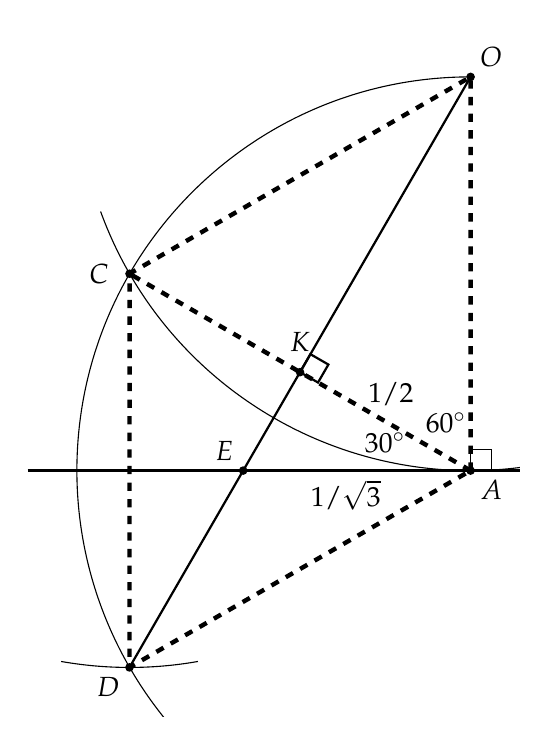
\begin{tikzpicture}[scale=1.25]
% Scale at 4

\clip (-4.5,-6.5) rectangle +(5,7);
% Coordinates of circle
\coordinate (O) at (0,0);
\coordinate (A) at (0,-4);
\coordinate (B) at (0,4);

% Draw circle
\node [circle through=(A),name path=circle] at (O) {};
\draw ($(O)+(200:4)$) arc [start angle=200,end angle=280,radius=4];

% Draw tangent at A
\draw[thick,name path=tangent] ($(A)+(-4.5,0)$) -- ($(A)+(10.5,0)$);
\draw (A) rectangle +(6pt,6pt);

% Draw arc centered at O which intersects circle at C
\draw[thin,name path=Aarc] (O)
   arc [start angle=90,end angle=220,radius=4];
\path[name intersections={of=circle and Aarc,by=C}];

% Draw arc centered at C which intersects the first arc at D
\draw[thin,name path=Carc] ($(C)+(260:4)$)
   arc [start angle=260,end angle=280,radius=4];
\path[name intersections={of=Carc and Aarc,by=D}];

% Draw O--D which intersects the tangent at E
\draw[thick,name path=OD] (O) -- (D);
\path[name intersections={of=tangent and OD,by=E}];

% Find point H at length 3 from E
\coordinate (F) at ($(E)+(4,0)$);
\coordinate (G) at ($(F)+(4,0)$);
\coordinate (H) at ($(G)+(4,0)$);

% Draw BH of length approximately pi
\draw[thick] (B) -- (H);

\draw[ultra thick,dashed] (A) -- (O) -- (C) -- (D) -- cycle;
\draw[ultra thick,dashed,name path=AC] (A) -- (C);

\node[above left,yshift=10pt,xshift=2pt] at (A) {$60^\circ$};
\node[left,yshift=10pt,xshift=-20pt] at (A) {$30^\circ$};

\path[name intersections={of=AC and OD,by=K}];
\draw[thick,rotate=-30] (K) rectangle +(6pt,6pt);

\path (A) -- node[above,xshift=2pt,yshift=2pt] {$1/2$} (K);
\path (A) -- node[below,xshift=-4pt] {$1/\sqrt{3}$} (E);

\fill (O) circle(1.25pt) node[above right] {$O$};
\fill (A) circle(1.25pt) node[below right] {$A$};
\fill (B) circle(1.25pt) node[above right] {$B$};
\fill (C) circle(1.25pt) node[left,xshift=-4pt] {$C$};
\fill (D) circle(1.25pt) node[below left] {$D$};
\fill (E) circle(1.25pt) node[above left] {$E$};
\fill (F) circle(1.25pt) node[above right,xshift=4pt] {$F$};
\fill (G) circle(1.25pt) node[above] {$G$};
\fill (H) circle(1.25pt) node[above] {$H$};
\fill (K) circle(1.25pt) node[above,yshift=4pt] {$K$};
\end{tikzpicture}
\end{center}
האלכסון
$\overline{AC}$
מייצר שני משולשים שווי-צלעות
$\triangle OAC, \triangle DAC$
כך ש-%
$\angle OAC=60^\circ$.
הזווית בין המשיק לרדיוס
$\overline{OA}$
היא זווית ישרה ולכן
$\angle KAE=30^\circ$.
נחשב:
\begin{displaymath}
\renewcommand{\arraystretch}{1.5}
\begin{array}{lcl}
\disfrac{1/2}{\overline{EA}}&=&
\cos 30^\circ=\disfrac{\sqrt{3}}{2}\\
\overline{EA}&=&\disfrac{1}{\sqrt{3}}\\
\overline{AH}&=&3-\overline{EA}=\left(3-\disfrac{1}{\sqrt{3}}\right)
=\disfrac{3\sqrt{3}-1}{\sqrt{3}}\\
\end{array}
\end{displaymath}
נחזור לאיור הראשון ונראה ש-%
$\triangle ABH$
הוא משולש ישר-זווית:
\begin{displaymath}
\renewcommand{\arraystretch}{1.5}
\begin{array}{lcl}
\overline{BH}^2&=&\overline{OB}^2+\overline{AH}^2\\
&=&4+\disfrac{9\cdot 3 -6\sqrt{3}+1}{3}=\disfrac{40}{3}-2\sqrt{3}\\
\overline{BH}&=&\sqrt{\disfrac{40}{3}-2\sqrt{3}}\approx 3.141533387=\approx \pi\,.
\end{array}
\end{displaymath}


%%%%%%%%%%%%%%%%%%%%%%%%%%%%%%%%%%%%%%%%%%%%%%%%%%%%%%%%%%%%%%%%%%%

\vspace*{-16ex}

\section{הבנייה הראשונה של
\L{Ramanujan}}


\subsection{הבניה}

בנו מעגל יחידה שמרכזו 
$O$
וסמנו קוטר
$\overline{PR}$.

$H$
חוצה את
$\overline{PO}$
ו-%
$T$
מחלק את
$\overline{RO}$
לשלושה חלקים שווים.

בנו ניצב ב-%
$T$
שחותך את המעגל ב-%
$Q$.

בנו את המיתר
$\overline{RS}=\overline{QT}$.

בנו את קטע הקו
$\overline{PS}$.

בנו קו העובר דרך
$T$
המקביל ל-%
$RS$.
סמנו ב-%
$N$
את החיתוך של עם 
$\overline{PS}$.

בנו קו העובר דרך
$O$
המקביל ל-%
$RS$.
סמנו ב-%
$M$
את החיתוך של עם 
$\overline{PS}$.

בנו את המיתר
$\overline{PK}=\overline{PM}$.

בנו משיק ב-%
$P$
שאורכו
$\overline{PL}=\overline{MN}$.

חברו את הנקודות
$K,L,R$.

מצאו נקודה 
$C$
כך שאורכו של
$\overline{RC}$
שווה לאורכו של
$\overline{RH}$.

בנו קטע קו
$\overline{CD}$
המקביל ל-%
$\overline{KL}$
שחותך את
$\overline{LR}$ 
ב-%
$D$. 

טענה:
$\overline{RD}^2=\disfrac{355}{113}\approx pi$.

\begin{center}
\selectlanguage{english}
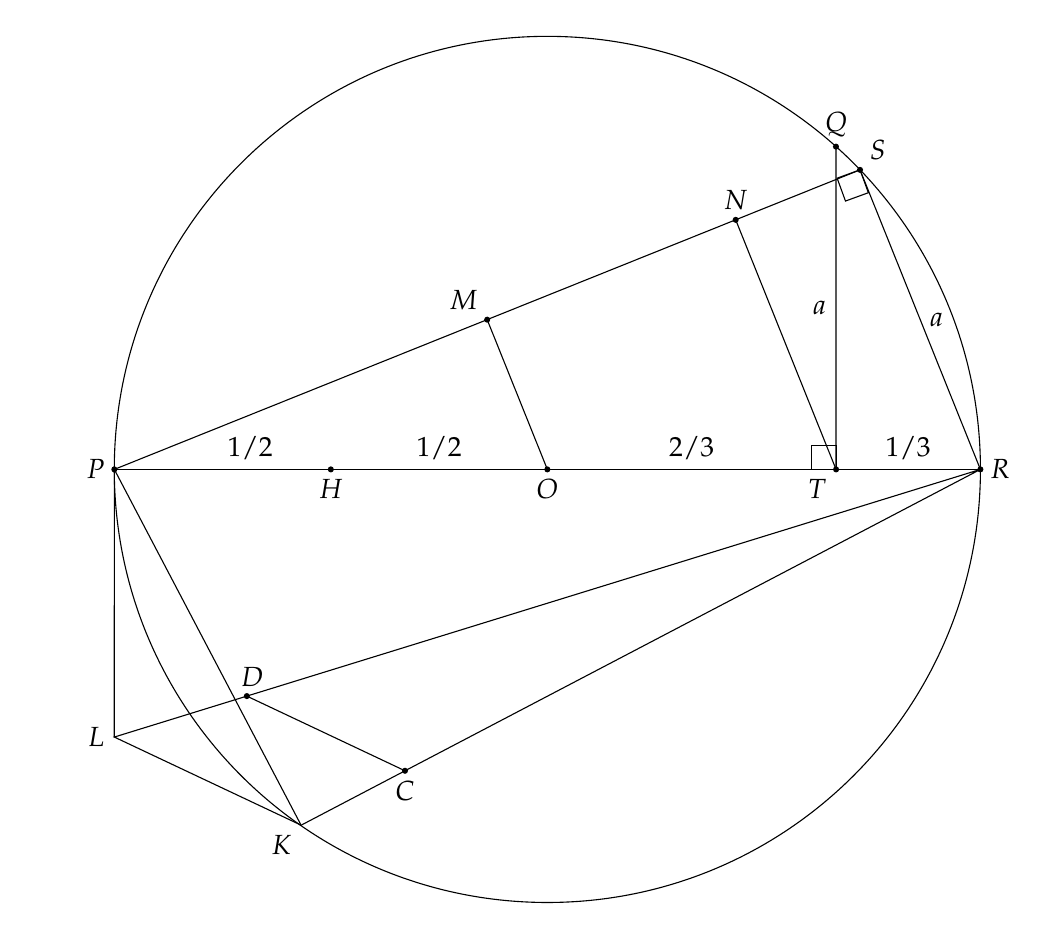
\begin{tikzpicture}[scale=1.1,align=left]
\clip (-6,-5.1) rectangle +(11.5,10.2);
% Draw circle and horizontal diameter
\draw[name path=circle] (0,0)  coordinate (o) node[below] {$O$} circle[radius=5cm];
\draw (-5,0) coordinate (p) node[left] {$P$} -- (5,0) coordinate (r) node[right] {$R$};
\fill (o) circle (1pt);
\fill (p) circle (1pt);
\fill (r) circle (1pt);
\fill (-2.5,0) coordinate (h) node[below] {$H$} circle (1pt);
\fill (10/3,0) coordinate (t) node[below left] {$T$} circle (1pt);
\path (p) -- node[above,xshift=10pt] {$1/2$} (h) -- node[above] {$1/2$} (o) -- node[above] {$2/3$} (t) -- node[above] {$1/3$} (r);

% Draw perpendicular TQ
\path[name path=tq] (t) -- +(0,5);
\path[name intersections={of=tq and circle,by=q}];
\draw (t) -- node[left] {$a$} (q) node[above] {$Q$};
\fill (q) circle (1pt);

% Draw chord RS and line PS
\path[name path=tq] (t) -- +(0,5);
\path[name intersections={of=tq and circle,by=q}];
\path[name path=rcirc] (r) let \p1 = ($ (t) - (q) $) in circle ({veclen(\x1,\y1)});
\path[name intersections={of=rcirc and circle,by=s}];
\draw (r) -- node[right] {$a$} (s);
\fill (s) node[above right] {$S$} circle (1pt);
\draw[name path=ps] (p) -- (s);

% Draw TN
\path[name path=tn] (t) -- +($(s)-(r)$);
\path[name intersections={of=ps and tn,by=n}];
\draw (t) -- (n);
\fill (n) node[above] {$N$} circle (1pt);

% Draw OM
\path[name path=om] (o) -- +($(s)-(r)$);
\path[name intersections={of=ps and om,by=m}];
\draw (o) -- (m);
\fill (m) node[above left] {$M$} circle (1pt);
\path (p) -- (m);
\path (m) -- (n);

% Draw chord PK
\draw (p) -- +(-62.3:4.64) coordinate (k) node[below left] {$K$};

% Draw tangent PL
\draw let \p1 = ($ (m) - (n) $), \n1 = {veclen(\x1,\y1)} in (p) -- (-5,-\n1) coordinate (l) node[left] {$L$};

% Connect L and K to R
\draw (r) -- (l) -- (k) -- cycle;

% Find point C on RK
\coordinate (c) at ($(r)!7.5cm!(k)$);
\path (r) -- (c);
\fill (c) node[below] {$C$} circle (1pt);

% Draw CD
\path[name path=cd] (c) -- +($(l)-(k)$);
\path[name path=lr] (l) -- (r);
\path[name intersections={of=cd and lr,by=d}];
\draw (c) -- (d);
\fill (d) node[above,xshift=2pt] {$D$} circle (1pt);
\path (r) -- (d);

\draw[rotate=90] (t) rectangle +(8pt,8pt);
\draw[rotate=-160] (s) rectangle +(8pt,8pt);
\end{tikzpicture}
\end{center}

\newpage

\subsection{ההוכחה}

לפי משפט פיתגורס במשולש ישר-הזווית
$\triangle QOT$:
\[
\overline{QT} = \sqrt{1^2-\left(\frac{2}{3}\right)^2}=\frac{\sqrt{5}}{3}\,.
\]
$\triangle PSR$
הוא משולש ישר-זווית כי הוא נשען על קוטר. לפי משפט פיתגורס:
\[
\overline{PS} = \sqrt{2^2-\left(\frac{\sqrt{5}}{3}\right)^2}=\sqrt{4-\frac{5}{9}}=\frac{\sqrt{31}}{3}\,.
\]
$\triangle MPO\sim \triangle SPR$
ולכן:
\begin{form}{1.5}
\disfrac{\overline{PM}}{\overline{PO}}&=&\disfrac{\overline{PS}}{\overline{PR}}\\
\disfrac{\overline{PM}}{1}&=&\disfrac{\sqrt{31}/3}{2}\\
\overline{PM}&=&\disfrac{\sqrt{31}}{6}\,.
\end{form}
$\triangle NPT\sim \triangle SPR$
ולכן:
\begin{form}{1.5}
\disfrac{\overline{PN}}{\overline{PT}}&=&\disfrac{\overline{PS}}{\overline{PR}}\\
\disfrac{\overline{PN}}{5/3}&=&\disfrac{\sqrt{31}/3}{2}\\
\overline{PN}&=&\disfrac{5\sqrt{31}}{18}\\
\overline{MN}&=&\overline{PN}-\overline{PM}\\
&=&\sqrt{31}\left(\disfrac{5}{18}-\disfrac{1}{6}\right) = \disfrac{\sqrt{31}}{9}\,.
\end{form}
$\triangle PKR$
הוא משולש ישר-זווית כי הוא נשען על קוטר. לפי משפט פיתגורס:
\[
\overline{RK}=\sqrt{2^2-\left(\frac{\sqrt{31}}{6}\right)^2} = \frac{\sqrt{113}}{6}\,.
\]
$\triangle PLR$
הוא משולש ישר-זווית כי 
$\overline{PL}$
הוא משיק. לפי משפט פיתגורס:
\[
\overline{RL}=\sqrt{2^2+\left(\frac{\sqrt{31}}{9}\right)^2} = \frac{\sqrt{355}}{9}\,.
\]

\newpage

$\overline{RC}=\overline{RH}=\displaystyle\frac{1}{3}+\frac{2}{3}+\frac{1}{2}=\frac{3}{2}$.
$\overline{CD}$
מקביל ל-%
$\overline{LK}$,
ולכן לפי משולשים דומים:
\begin{form}{1.5}
\disfrac{\overline{RD}}{\overline{RC}}&=&\disfrac{\overline{RL}}{\overline{RK}}\\
\disfrac{\overline{RD}}{3/2}&=&\disfrac{\sqrt{355}/9}{\sqrt{113}/6}\\
\overline{RD}&=&\sqrt{\disfrac{355}{113}}\,.
\end{form}

באיור להלן כל אורכי קטעי הקו מסומנים:
\begin{center}
\selectlanguage{english}
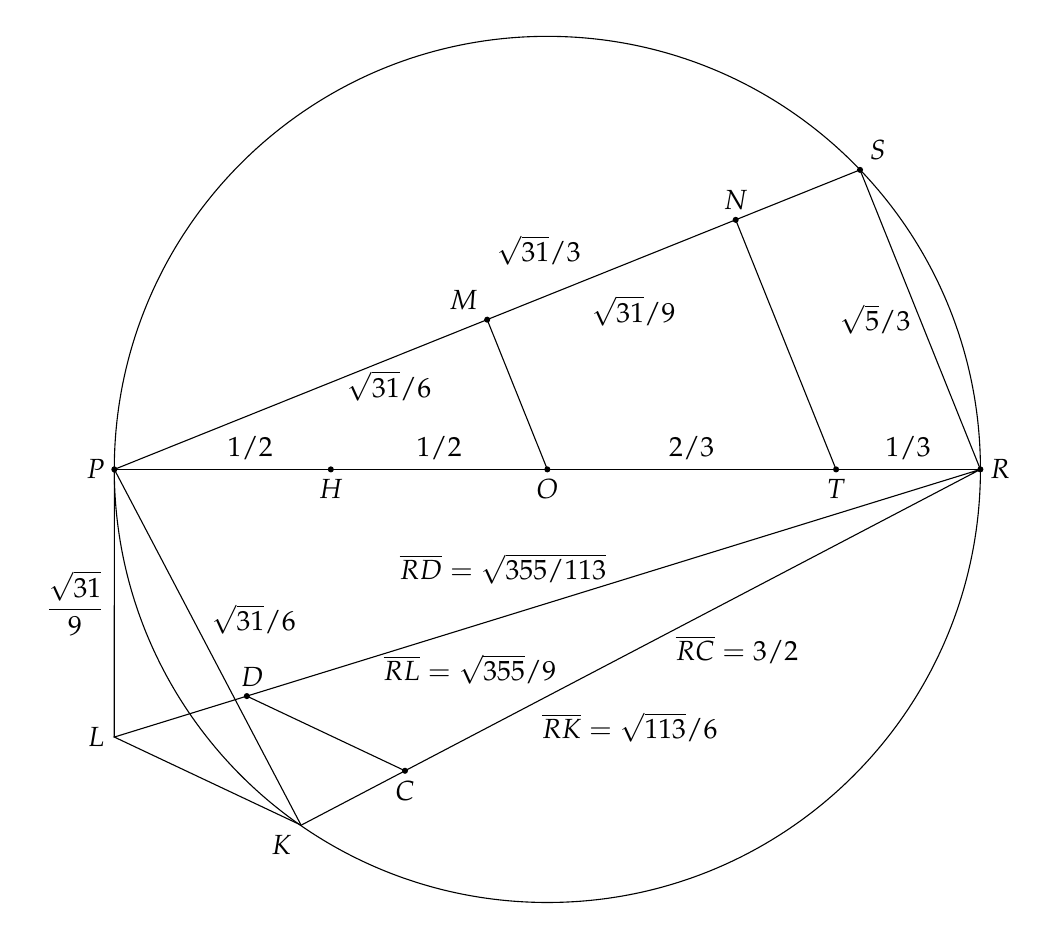
\begin{tikzpicture}[scale=1.1,align=left]
\clip (-6,-5.1) rectangle +(11.5,10.2);
% Draw circle and horizontal diameter
\draw[name path=circle] (0,0)  coordinate (o) node[below] {$O$} circle[radius=5cm];
\draw (-5,0) coordinate (p) node[left] {$P$} -- (5,0) coordinate (r) node[right] {$R$};
\fill (o) circle (1pt);
\fill (p) circle (1pt);
\fill (r) circle (1pt);
\fill (-2.5,0) coordinate (h) node[below] {$H$} circle (1pt);
\fill (10/3,0) coordinate (t) node[below] {$T$} circle (1pt);
\path (p) -- node[above,xshift=10pt] {$1/2$} (h) -- node[above] {$1/2$} (o) -- node[above] {$2/3$} (t) -- node[above] {$1/3$} (r);
% Draw chord RS and line PS
\path[name path=tq] (t) -- +(0,5);
\path[name intersections={of=tq and circle,by=q}];
\path[name path=rcirc] (r) let \p1 = ($ (t) - (q) $) in circle ({veclen(\x1,\y1)});
\path[name intersections={of=rcirc and circle,by=s}];
\draw (r) -- node[left] {$\sqrt{5}/3$} (s);
\fill (s) node[above right] {$S$} circle (1pt);
\draw[name path=ps] (p) -- node[above right,yshift=16pt] {$\sqrt{31}/3$} (s);
% Draw TN
\path[name path=tn] (t) -- +($(s)-(r)$);
\path[name intersections={of=ps and tn,by=n}];
\draw (t) -- (n);
\fill (n) node[above] {$N$} circle (1pt);
% Draw OM
\path[name path=om] (o) -- +($(s)-(r)$);
\path[name intersections={of=ps and om,by=m}];
\draw (o) -- (m);
\fill (m) node[above left] {$M$} circle (1pt);
\path (p) -- node[below,xshift=32pt,yshift=12pt] {$\sqrt{31}/6$} (m);
\path (m) -- node[below,xshift=8pt,yshift=-6pt] {$\sqrt{31}/9$} (n);
% Draw chord PK
\draw (p) -- node[right,xshift=-2pt,yshift=10pt] {$\sqrt{31}/6$} +(-62.3:4.64) coordinate (k) node[below left] {$K$};
% Draw tangent PL
\draw let \p1 = ($ (m) - (n) $), \n1 = {veclen(\x1,\y1)} in (p) -- node[left] {$\disfrac{\sqrt{31}}{9}$} (-5,-\n1) coordinate (l) node[left] {$L$};
% Connect L and K to R
\draw (r) -- (l) -- (k) -- cycle;
% Find point C on RK
\coordinate (c) at ($(r)!7.5cm!(k)$);
%\path (r) -- node[below,yshift=-16pt] {$RC=3/2$\\$RK=\sqrt{113}/6$} (c);
\path (r) -- node[below,xshift=16pt,yshift=-2pt] {$\overline{RC}=3/2$} (c);
\path (r) -- node[below,xshift=-4pt,yshift=-20pt] {$\overline{RK}=\sqrt{113}/6$} (k);
\fill (c) node[below] {$C$} circle (1pt);
% Draw CD
\path[name path=cd] (c) -- +($(l)-(k)$);
\path[name path=lr] (l) -- (r);
\path[name intersections={of=cd and lr,by=d}];
\draw (c) -- (d);
\fill (d) node[above,xshift=2pt] {$D$} circle (1pt);
%\path (r) -- node[above,xshift=-40pt,yshift=-8pt] {$RD=\sqrt{355/113}$\\$RL=\sqrt{355}/9$} (d);
\path (r) -- node[above,xshift=-40pt,yshift=-4pt] {$\overline{RD}=\sqrt{355/113}$} (d);
\path (r) -- node[below,xshift=-28pt,yshift=-15pt] {$\overline{RL}=\sqrt{355}/9$} (l);
\end{tikzpicture}
\end{center}

\bigskip

ניתן לבנות את ערך
$\disfrac{355}{113}$
על ידי בניית שני קטעי קו באורכים
$355$
ו-%
$113$,
ואז להשתמש בבנייה לחילוק מסעיף%
~\ref{s.square-intro},
אבל זה די מעיק!

\newpage

%%%%%%%%%%%%%%%%%%%%%%%%%%%%%%%%%%%%%%%%%%%%%%%%%%%%%%%%%%%

\section{הבנייה השנייה של
\L{Ramanujan}}


\subsection{הבניה}

בנו מעגל יחידה שמרכזו
$O$
עם קוטר
$\overline{AB}$,
וסמנו ב-%
$C$
את החיתוך של הניצב ב-%
$O$
עם המעגל.

חלקו את
$\overline{AO}$
לשלושה חלקים שווים כך ש-%
$\overline{AT}=1/3$ 
ו-%
$\overline{TO}=2/3$.

בנו
$\overline{BC}$
ןמצאו נקודות
$M,N$
כך ש-%
$\overline{CM}=\overline{MN}=\overline{AT}=1/3$.

בנו 
$\overline{AM}$
ו-%
$\overline{AN}$
וסמנו ב-%
$P$
את הנקודה על
$\overline{AN}$
כך ש-%
$\overline{AP}=\overline{AM}$.

בנו קו המקביל ל-%
$\overline{MN}$
שעובר דרך
$P$,
וסמנו ב-%
$Q$
את נקודת החיתוך שלו עם
$\overline{AM}$.

בנו
$\overline{OQ}$
ובנו קו המקביל ל-%
$\overline{OQ}$
שעובר דרך 
$T$ 
וסמנו ב-%
$R$
את נקודת החיתוך שלו עם
$\overline{AM}$.

בנו קטע קו 
$\overline{AS}$
שאורכו שווה לאורך של
$\overline{AR}$
והמשיק למעגל ב-%
$A$.

בנו
$\overline{SO}$.

טענה:
$3\sqrt{\overline{SO}}=\left(9^2+\disfrac{19^2}{22}\right)^{\frac{1}{4}}\approx \pi$.

\begin{center}
\selectlanguage{english}
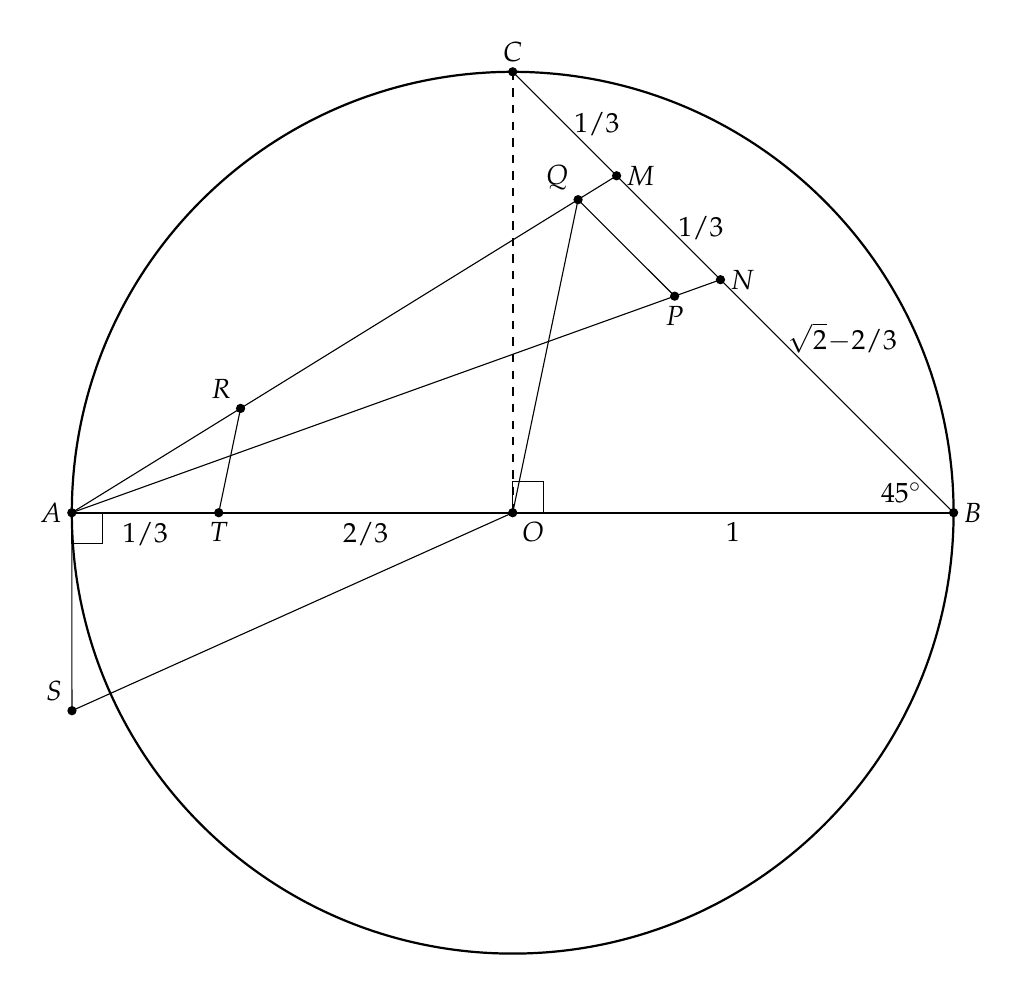
\begin{tikzpicture}[scale=1.4]
\clip (-4.4,-4.2) rectangle +(8.8,8.6);
% Scale at 4

% Coordinates of circle
\coordinate (O) at (0,0);
\coordinate (A) at (-4,0);
\coordinate (B) at (4,0);
\coordinate (C) at (0,4);

% Draw circle and diameter
\node [thick,draw,circle through=(A),name path=circle] at (O) {};
\draw [thick] (A) -- (B);
\draw [thick,dashed] (C) -- (O);
\draw (O) rectangle +(8pt,8pt);
\draw[rotate=-90] (A) rectangle +(8pt,8pt);

\coordinate (T) at (-2.667,0);
\path (A) -- node[below] {$1/3$} (T);
\path (T) -- node[below] {$2/3$} (O);
\path (O) -- node[below] {$1$} (B);

\draw (C) -- node[right] {$1/3$} +(-45:1.333) coordinate (M);
\draw (M) -- node[right] {$1/3$} +(-45:1.333) coordinate (N);
\draw (N) -- node[near start,right] {$\sqrt{2}\!-\!2/3$}(B);

\draw[name path=AM] (A) -- (M);
\draw[name path=AN] (A) -- (N);

\node [circle through=(M),name path=AMcircle] at (A) {};

\path[name intersections={of=AMcircle and AN,by=P}];

\path[name path=PQ] (P) -- +(135:2);
\path[name intersections={of=PQ and AM,by=Q}];
\draw (P) -- (Q) -- (O);

\path[name path=QT] (T) -- ($(Q)+(-2.667,0)$) -- (Q);
\path[name intersections={of=QT and AM,by=R}];
\draw (T) -- (R);

\node [circle through=(R),name path=ARcircle] at (A) {};
\path[name path=AS] (A) -- ($(A)+(0,-2.5)$);
\path[name intersections={of=ARcircle and AS,by=S}];
\draw (A) -- (S);

\draw (S) -- (O);

\fill (O) circle(1.2pt) node[below right] {$O$};
\fill (A) circle(1.2pt) node[left] {$A$};
\fill (B) circle(1.2pt) node[right] {$B$} node[above left,xshift=-8pt] {$45^\circ$};
\fill (C) circle(1.2pt) node[above] {$C$};
\fill (T) circle(1.2pt) node[below] {$T$};
\fill (M) circle(1.2pt) node[right] {$M$};
\fill (N) circle(1.2pt) node[right] {$N$};
\fill (P) circle(1.2pt) node[below] {$P$};
\fill (Q) circle(1.2pt) node[above left] {$Q$};
\fill (R) circle(1.2pt) node[above left] {$R$};
\fill (S) circle(1.2pt) node[above left] {$S$};

\end{tikzpicture}
\end{center}

\newpage

\subsection{ההוכחה}

$\triangle COB$
הוא משולש ישר זווית,
$\overline{OB}=\overline{OC}=1$,
ןלכן לפי משפט פיתגורס
$\overline{CB}=\sqrt{2}$
ו-%
$\overline{NB}=\sqrt{2}-2/3$.
המשולש שווה שוקיים, כך ש-%
$\angle NBA =\angle MBA=45^\circ$.

נשתמש במשפט הקוסינוסים על 
$\triangle NBA$
כדי לחשב את
$\overline{AN}$:
\begin{form}{1}
\overline{AN}^2&=&\overline{BA}^2 + \overline{BN}^2-2\cdot\overline{BA}\cdot\overline{BN}\cdot\cos \angle NBA\\
&=&2^2+\left(\sqrt{2}-\disfrac{2}{3}\right)^2-2\cdot 2 \cdot \left(\sqrt{2}-\disfrac{2}{3}\right)\cdot \disfrac{\sqrt{2}}{2}\\
&=&\left(4+2+\disfrac{4}{9}-4\right) + \sqrt{2}\cdot \left(-\disfrac{4}{3}+\disfrac{4}{3}\right)=\disfrac{22}{9}\\
\overline{AN}&=&\sqrt{\disfrac{22}{9}}\,.
\end{form}
באופן דומה, נשתמש במשפט הקוסינוסים על
$\triangle MBA$
כדי לחשב את
$\overline{AM}$:
\begin{form}{1.2}
\overline{AM}^2&=&\overline{BA}^2 + \overline{BM}^2-2\cdot\overline{BA}\cdot\overline{BM}\cdot\cos \angle MBA\\
&=&2^2+\left(\sqrt{2}-\disfrac{1}{3}\right)^2-2\cdot 2 \cdot \left(\sqrt{2}-\disfrac{1}{3}\right)\cdot \disfrac{\sqrt{2}}{2}\\
&=&\left(4+2+\disfrac{1}{9}-4\right) + \sqrt{2}\cdot \left(-\disfrac{2}{3}+\disfrac{2}{3}\right)=\disfrac{19}{9}\\
\overline{AM}&=&\sqrt{\disfrac{19}{9}}\,.
\end{form}
לפי הבנייה
$\overline{QP}\parallel \overline{MN}$
ולכן
$\triangle MAN\sim \triangle QAP$,
ולפי הבנייה
$\overline{AP}=\overline{AM}$,
כך ש:
\begin{form}{1.5}
\disfrac{\overline{AQ}}{\overline{AM}}&=&\disfrac{\overline{AP}}{\overline{AN}}=\disfrac{\overline{AM}}{\overline{AN}}\\
\overline{AQ}&=&\disfrac{\overline{AM}^2}{\overline{AN}}=\disfrac{19/9}{\sqrt{22/9}}=\disfrac{19}{3\sqrt{22}}\,.
\end{form}

לפי הבנייה
$\overline{TR}\parallel \overline{OQ}$
ולכן
$\triangle RAT\sim \triangle QAO$
כך ש:
\begin{form}{1.2}
\disfrac{\overline{AR}}{\overline{AQ}}&=&\disfrac{\overline{AT}}{\overline{AO}}\\
\overline{AR}&=&\overline{AQ}\cdot\disfrac{\overline{AT}}{\overline{AO}}=\disfrac{19}{3\sqrt{22}}\cdot\disfrac{1/3}{1}=\disfrac{19}{9\sqrt{22}}\,.
\end{form}

\newpage
לפי הבנייה
$\overline{AS}=\overline{AR}$
ו-%
$\triangle OAS$ 
הוא משולש ישר זווית. לפי משפט פיתגורס:
\begin{form}{1.5}
\overline{SO}&=&\sqrt{1^2+\left(\disfrac{19}{9\sqrt{22}}\right)^2}\\
3\sqrt{\overline{SO}}&=&3\left(1+\disfrac{19^2}{9^2\cdot 22}\right)^\frac{1}{4}\\
&=&\left(3^4+\disfrac{3^4\cdot 19^2}{9^2\cdot 22}\right)^\frac{1}{4}\\
&=&\left(9^2+\disfrac{19^2}{22}\right)^\frac{1}{4}\approx 3.14159265262\approx \pi\,.
\end{form}

באיור להלן כל אורכי קטעי הקו מסומנים:
\begin{center}
\selectlanguage{english}
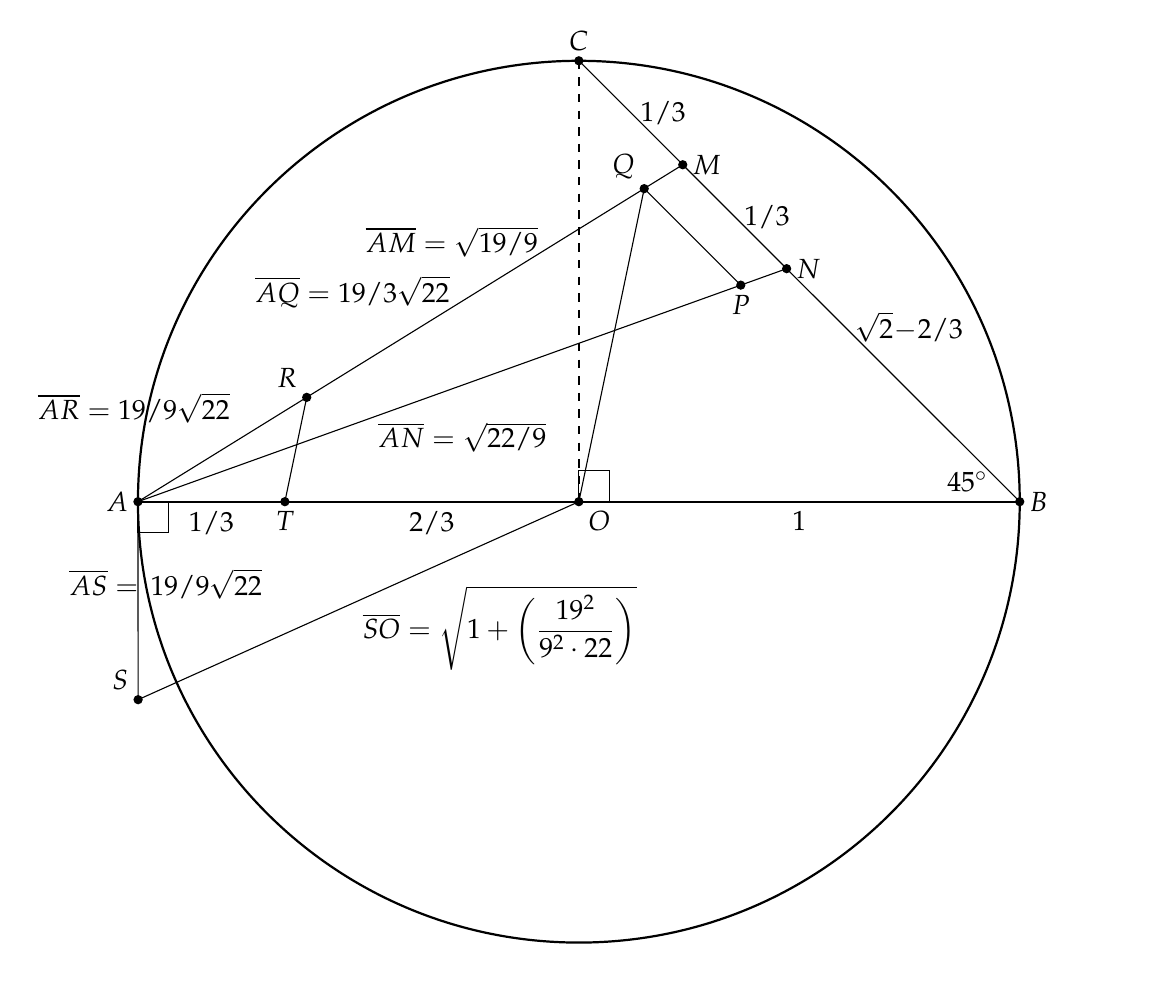
\begin{tikzpicture}[scale=1.4]
\clip (-5,-4.2) rectangle +(10,8.5);
% Scale at 4

% Coordinates of circle
\coordinate (O) at (0,0);
\coordinate (A) at (-4,0);
\coordinate (B) at (4,0);
\coordinate (C) at (0,4);

% Draw circle and diameter
\node [thick,draw,circle through=(A),name path=circle] at (O) {};
\draw [thick] (A) -- (B);
\draw [thick,dashed] (C) -- (O);
\draw (O) rectangle +(8pt,8pt);
\draw[rotate=-90] (A) rectangle +(8pt,8pt);

\coordinate (T) at (-2.667,0);
\path (A) -- node[below] {$1/3$} (T);
\path (T) -- node[below] {$2/3$} (O);
\path (O) -- node[below] {$1$} (B);

\draw (C) -- node[right] {$1/3$} +(-45:1.333) coordinate (M);
\draw (M) -- node[right] {$1/3$} +(-45:1.333) coordinate (N);
\draw (N) -- node[near start,right] {$\sqrt{2}\!-\!2/3$}(B);

\draw[name path=AM] (A) -- node[above,xshift=15pt,yshift=24pt] {$\overline{AM}=\sqrt{19/9}$} (M);
\draw[name path=AN] (A) -- node[below,yshift=-10pt] {$\overline{AN}=\sqrt{22/9}$} (N);

\node [circle through=(M),name path=AMcircle] at (A) {};

\path[name intersections={of=AMcircle and AN,by=P}];

\path[name path=PQ] (P) -- +(135:2);
\path[name intersections={of=PQ and AM,by=Q}];
\draw (P) -- (Q) -- (O);
\path (A) -- node[above,xshift=-14pt,yshift=10pt] {$\overline{AQ}=19/3\sqrt{22}$} (Q);

\path[name path=QT] (T) -- ($(Q)+(-2.667,0)$) -- (Q);
\path[name intersections={of=QT and AM,by=R}];
\draw (T) -- (R);
\path (A) -- node[above,xshift=-32pt,yshift=6pt] {$\overline{AR}=19/9\sqrt{22}$} (R);

\node [circle through=(R),name path=ARcircle] at (A) {};
\path[name path=AS] (A) -- ($(A)+(0,-2.5)$);
\path[name intersections={of=ARcircle and AS,by=S}];
\draw (A) -- node[xshift=10pt,yshift=6pt] {$\overline{AS}=\,19/9\sqrt{22}$} (S);

\draw (S) -- node[right,xshift=-2pt,yshift=-10pt] {$\overline{SO}=\sqrt{1+
  \left(\disfrac{19^2}{9^2\cdot 22}\right)}$} (O);

\fill (O) circle(1.2pt) node[below right] {$O$};
\fill (A) circle(1.2pt) node[left] {$A$};
\fill (B) circle(1.2pt) node[right] {$B$} node[above left,xshift=-8pt] {$45^\circ$};
\fill (C) circle(1.2pt) node[above] {$C$};
\fill (T) circle(1.2pt) node[below] {$T$};
\fill (M) circle(1.2pt) node[right] {$M$};
\fill (N) circle(1.2pt) node[right] {$N$};
\fill (P) circle(1.2pt) node[below] {$P$};
\fill (Q) circle(1.2pt) node[above left] {$Q$};
\fill (R) circle(1.2pt) node[above left] {$R$};
\fill (S) circle(1.2pt) node[above left] {$S$};

\end{tikzpicture}
\end{center}


\tikzsetfigurename{compass-only}
% !TeX root = construct.tex


\selectlanguage{hebrew}


\chapter{אני מסתפק במחוגה}\label{c.compass-only}

%%%%%%%%%%%%%%%%%%%%%%%%%%%%%%%%%%%%%%%%%%%%%%%%%%%%%%%%%%%%%%%

בשנת
$1797$
המתימטיקאי האיטלקי
\L{Lorenzo Mascheroni}
הוכיח שכל בנייה גיאומטרית עם סרגל ומחוגה ניתנת לבנייה עם מחוגה בלבד! במאה העשרים התגלה שהמשפט הוכח בשנת
$1672$
על ידי המתימטיקאי הדני
\L{Georg Mohr}.
המשפט נקרא היום משפט
\L{Mohr-Mascheroni}.

בפרק זה אביא את הוכחת המשפט המבוססת על הוכחה שמופיעה כבעייה
$33$
ב-%
\L{\cite{dorrie1}},
ועובדה על ידי
\L{Michael Woltermann} \L{\cite{dorrie2}}.%
\footnote{%
ברצוני להודות לו על הרשות להתשמש בעבודתו.
}
הוכחות נוספות ניתן למוצא ב-%
\L{\cite{mm}}, \L{\cite{stopel}}.

מה המשמעות של בנייה גיאומטרית עם מחוגה בלבד ללא סרגל? התרשים הימני מראה את הבנייה הרגילה של משולש שווה צלעות עם סרגל ומחוגה. איך אפשר לבנות משולש ללא קטעי הקווים
$AB,AC,BC$?
למעשה, אין כל צורך
\textbf{לראות}
את הקווים. קו מוגדר על ידי שתי נקודות, ומספיק שנבנה את נקודות כדי לקבל בנייה שקולה לבנייה עם סרגל )התרשים השמאלי(.

\begin{center}
\selectlanguage{english}
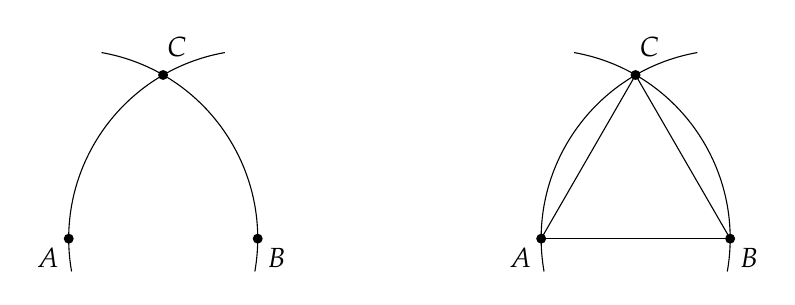
\begin{tikzpicture}[scale=0.6]
\coordinate (A) at (0,0);
\coordinate (B) at (4,0);
\path (A) node[below left] {$A$} -- (B) node[below right] {$B$};
\fill (A) circle[radius=3pt];
\fill (B) circle[radius=3pt];
\draw[name path=larc] (A) ++(-10:4cm) arc (-10:80:4cm);
\draw[name path=rarc] (B) ++(-170:4cm) arc (-170:-260:4cm);
\path [name intersections={of=larc and rarc,by={t}}];
\fill (t) node[above right,xshift=-2pt,yshift=3pt] {$C$} circle[radius=3pt];
\begin{scope}[xshift=10cm]
\coordinate (A) at (0,0);
\coordinate (B) at (4,0);
\draw (A) node[below left] {$A$} -- (B) node[below right] {$B$};
\fill (A) circle[radius=3pt];
\fill (B) circle[radius=3pt];
\draw[name path=larc] (A) ++(-10:4cm) arc (-10:80:4cm);
\draw[name path=rarc] (B) ++(-170:4cm) arc (-170:-260:4cm);
\path [name intersections={of=larc and rarc,by={t}}];
\fill (t) node[above right,xshift=-2pt,yshift=3pt] {$C$} circle[radius=3pt];
\draw (A) -- (t);
\draw (B) -- (t);
\end{scope}
\end{tikzpicture}
\selectlanguage{hebrew}
\end{center}
בתרשימים נצייר בכל זאת קווים, אולם הקווים משמשים אך ורק להבנת הבנייה ולהוכחת נכונותה. חשוב שתשתכנעו שבבנייה עצמה משתמשים רק במחוגה.


בבנייה עם סרגל ומחוגה מבצעת אחת משלוש פעולות הבאות:
\begin{itemize}
\item
מציאת נקודת החיתוך של שני קווים ישרים.
\item
מציאת נקודות החיתוך בין קו ישר ומעגל.
\item
מציאת נקודות החיתוך בין שני מעגלים.
\end{itemize}
ברור שניתן לבצע את הפעולה השלישית רק עם מחוגה. עלינו להראות שעבור שתי הפעולות הראשונות ניתן למוצא בנייה שקולה המשתמשת רק במחוגה.


סימונים:
\begin{itemize}
\item $C(O,A)$: 
המעגל שמרכזו
$O$
העובר דרך הנקודה
$A$.
\item $C(O,r)$:
המעגל שמרכזו
$O$
עם רדיוס
$r$.
\item $C(O,AB)$:
המעגל שמרכזו
$O$
עם רדיוס שהוא אורך קטע קו נתון
$AB$.
\end{itemize}

תחילה נביא ארבע בניות עזר נחוצות )סעיפים
\L{\ref{s.reflection}--\ref{s.relative}}%
(,
ואחר כך נראה את הבניות למציאת חיתוך של שני קווים )סעיף
\L{\ref{s.two-lines}}%
( ושל קו ומעגל )סעיף
\L{\ref{s.line-circle}}%
(.
%%%%%%%%%%%%%%%%%%%%%%%%%%%%%%%%%%%%%%%%%%%%%%%%%%%%%%%%%%%%%%%

\np

\section{%
שיקוף נקודה%
}\label{s.reflection}
\textbf{%
נתון קטע קו
$AB$
ונקודה 
$C$
שלא נמצאת על
$AB$.
ניתן לבנות נקודה 
$C'$
שהיא השיקוף של
$C$
מסביב ל-%
$AB$.
}
הנקודה
$C'$
היא
\textbf{%
שיקוף%
}
של הנקודה
$C$
מסביב לקטע קו
$AB$,
אם 
$AB$
)או הקו המכיל אותו( הוא האנך האמצעי של
$CC'$.

נבנה מעגל שמרכזו
$A$
העובר דרך
$C$
ומעגל שמרכזו
$B$
העובר דרך
$C$.
החיתוך של שני המעגלים הוא הנקודה
$C'$
שהיא השיקוף של
$C$.

\vspace{-1ex}

\begin{center}
\selectlanguage{english}
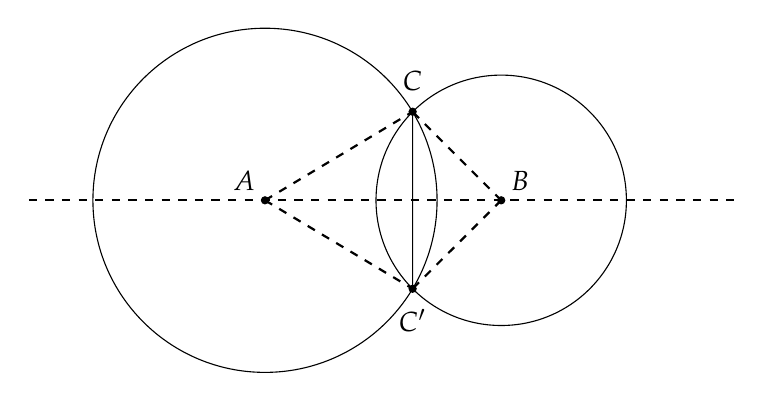
\begin{tikzpicture}[scale=.75]
\coordinate (A) at (0,0);
\coordinate (B) at (4,0);
\coordinate (C) at (2.5,1.5);
\draw[thick,dashed,name path=ab] ($(B)!2!(A)$) -- ($(A)!2!(B)$);
\fill (A) node[above left] {$A$} circle[radius=2pt];
\fill (B) node[above right] {$B$} circle[radius=2pt];
\fill (C) node[above,yshift=4pt] {$C$} circle[radius=2pt];
\node[draw,circle through=(C),name path=ac] at (A) {};
\node[draw,circle through=(C),name path=bc] at (B) {};
\path [name intersections={of=ac and bc,by={x1,Cp}}];
\fill (Cp) node[below,yshift=-4pt] {$C'$} circle[radius=2pt];
\draw (C) -- (Cp);
\draw[thick,dashed] (A) -- (C);
\draw[thick,dashed] (B) -- (C);
\draw[thick,dashed] (A) -- (Cp);
\draw[thick,dashed] (B) -- (Cp);
\end{tikzpicture}
\selectlanguage{hebrew}
\end{center}

\vspace{-1ex}

\textbf{הוכחה:}
$\triangle ABC$
ו-%
$\triangle ABC'$
חופפים לפי צ.צ.צ., כי
$AC,AC'$
הם רדיוסים של אותו מעגל כמו גם
$BC,BC'$,
ו-%
$AB$
הוא צלע משותף. מכאן ש-%
$\angle CAB = \angle C'AB$,
ולכן
$AB$
הוא חוצה הזווית של
$\angle CAC'$.
אבל
$\triangle CAC'$
הוא משולש שווה שוקיים, וחוצה הזווית
$AB$
הוא גם האנך האמצעי של בסיס המשולש
$CC'$.
לפי ההגדרה,
$C'$
היא השיקוף של
$C$
מסביב ל-%
$AB$.

\vspace{-2ex}

%%%%%%%%%%%%%%%%%%%%%%%%%%%%%%%%%%%%%%%%%%%%%%%%%%%%%%%%%%%%%%%

\section{%
בניית מעגל עם רדיוס נתון
}\label{s.radius}

\textbf{%
נתונות הנקודות
$A,B,C$.
ניתן לבנות מעגל
$c(A,BC)$
שמרכזו 
$A$
עם רדיוס שווה לאורך של 
$BC$.
}

נבנה את המעגלים 
$c(A,B)$, $c(B,A)$
ונסמן את נקודות החיתוך
$X,Y$.

\begin{center}
\selectlanguage{english}
\begin{tikzpicture}[scale=.65]
\coordinate (A) at (0,1.5);
\coordinate (B) at (0,-1.5);
\coordinate (C) at (1.5,-3);
\coordinate (Cp) at (1.5,3);
\fill (A) node[above] {$A$} circle[radius=3pt];
\fill (B) node[below] {$B$} circle[radius=3pt];
\fill (C) node[below] {$C$} circle[radius=3pt];
%\fill (Cp) node[above] {$C'$} circle[radius=3pt];
\node[draw,circle through=(B),name path=ab] at (A) {};
\node[draw,circle through=(A),name path=ba] at (B) {};
\path [name intersections={of=ab and ba,by={Y,X}}];
\fill (X) node[above right,xshift=4pt] {$X$} circle[radius=3pt];
\fill (Y) node[above left,xshift=-4pt] {$Y$} circle[radius=3pt];
\draw[thick,dashed] ($(X)!2.3!(Y)$) -- ($(Y)!2!(X)$);
%\draw[thick,dashed] (C) -- (Cp);
\end{tikzpicture}

\selectlanguage{hebrew}
\end{center}

\np


נבנה את
$C'$,
השיקוף של
$C$
מסביב לקו
$XY$
לפי הבנייה בסעיף
\L{\ref{s.reflection}}.
\begin{center}
\selectlanguage{english}
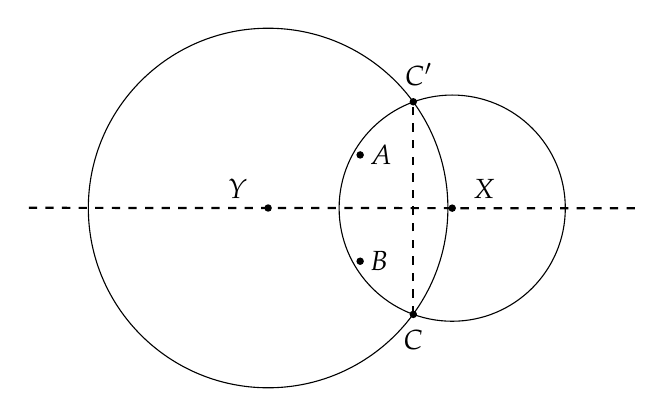
\begin{tikzpicture}[scale=.45]
\coordinate (A) at (0,1.5);
\coordinate (B) at (0,-1.5);
\coordinate (C) at (1.5,-3);
\coordinate (Cp) at (1.5,3);
\fill (A) node[right] {$A$} circle[radius=3pt];
\fill (B) node[right] {$B$} circle[radius=3pt];
\fill (C) node[below,yshift=-2pt] {$C$} circle[radius=3pt];
\fill (Cp) node[above,xshift=2pt,yshift=2pt] {$C'$} circle[radius=3pt];
\node[circle through=(B),name path=ab] at (A) {};
\node[circle through=(A),name path=ba] at (B) {};
\path [name intersections={of=ab and ba,by={Y,X}}];
\fill (X) node[above right,xshift=4pt] {$X$} circle[radius=3pt];
\fill (Y) node[above left,xshift=-4pt] {$Y$} circle[radius=3pt];
\node[draw,circle through=(C)] at (X) {};
\node[draw,circle through=(C)] at (Y) {};
\draw[thick,dashed] ($(X)!2.3!(Y)$) -- ($(Y)!2!(X)$);
%\draw (X) -- (Y) -- (C) -- (X) -- (Cp) -- (Y);
\draw[thick,dashed] (C) -- (Cp);
\end{tikzpicture}

\selectlanguage{hebrew}
\end{center}

המעגל
$c(A,C')$
הוא המעגל המבוקש.

\begin{center}

\selectlanguage{english}
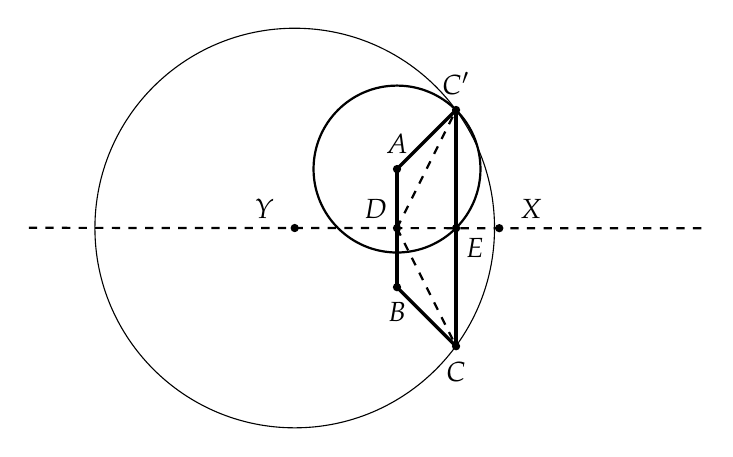
\begin{tikzpicture}[scale=.5]
\coordinate (A) at (0,1.5);
\coordinate (B) at (0,-1.5);
\coordinate (C) at (1.5,-3);
\coordinate (Cp) at (1.5,3);
\fill (A) node[above,yshift=2pt] {$A$} circle[radius=3pt];
\fill (B) node[below,yshift=-2pt] {$B$} circle[radius=3pt];
\fill (C) node[below,yshift=-2pt] {$C$} circle[radius=3pt];
\fill (Cp) node[above,yshift=2pt] {$C'$} circle[radius=3pt];
\node[circle through=(B),name path=ab] at (A) {};
\node[circle through=(A),name path=ba] at (B) {};
\path [name intersections={of=ab and ba,by={Y,X}}];
\fill (X) node[above right,xshift=4pt] {$X$} circle[radius=3pt];
\fill (Y) node[above left,xshift=-4pt] {$Y$} circle[radius=3pt];
\node[circle through=(C)] at (X) {};
\node[draw,circle through=(C)] at (Y) {};
\draw[thick,dashed] ($(X)!2.3!(Y)$) -- ($(Y)!2!(X)$);
\path[name path=xy] (X) -- (Y);
\node[draw,thick,circle through=(Cp)] at (A) {};
\draw[very thick] (A) -- (Cp);
\draw[very thick] (B) -- (C);
\draw[very thick,name path=abline] (A) -- (B);
\draw[very thick,name path=ccp] (C) -- (Cp);
\path [name intersections={of=xy and abline,by={D}}];
\path [name intersections={of=xy and ccp,by={E}}];
\fill (D) node[above left] {$D$} circle[radius=3pt];
\fill (E) node[below right] {$E$} circle[radius=3pt];
\draw[thick,dashed] (D) -- (Cp);
\draw[thick,dashed] (D) -- (C);
\end{tikzpicture}
\selectlanguage{hebrew}
\end{center}

\textbf{הוכחה:}
הנקודה
$A$
היא השיקוף של 
$B$
סביב 
$XY$
)כי
$\triangle YAX\cong \triangle YBX$(, ו-%
$C'$
נבנה כשיקוף של 
$C$
סביב
$XY$.
לפי ההגדרה, 
$XY$
הוא האנך האמצעי לקטעי הקו 
$AB$, $CC'$,
ולכן
$C'E=EC$,
$AD=DB$,
ו-%
$\angle DEC=\angle DEC'(=90^\circ)$.
מכאן ש-%
$\triangle DEC\cong\triangle DEC'$
לפי צ.ז.צ. לכן
$DC=DC'$
ו-%
$\angle ADC'=\angle BDC$
)כי הן זוויות משלימות ל-%
$\angle EDC, \angle EDC'$(.
$\triangle ADC'\cong\triangle BDC$
לפי צ.ז.צ.,
כך ש-%
$AC'=BC$.

ההוכחה מראה ששיקוף משמר מרחקים.

%%%%%%%%%%%%%%%%%%%%%%%%%%%%%%%%%%%%%%%%%%%%%%%%%%%%%%%%%%%%%%%

\section{%
בניית חיבור וחיסור של שני קטעי קווים%
}\label{s.add-subtract}

\textbf{%
נתון קטע קו
$PQ$
באורך
$a$
וקטע קו
$RS$
באורך
$b$.
ניתן לבנות קטעי קו
$QT,QU$
כך ש-%
$PUQT$
הוא קטע קו, כאשר האורך של
$PU$
הוא
$a-b$
והאורך של
$PT$
הוא
$a+b$.
}

\begin{center}
\selectlanguage{english}
%\vspace*{-2ex}
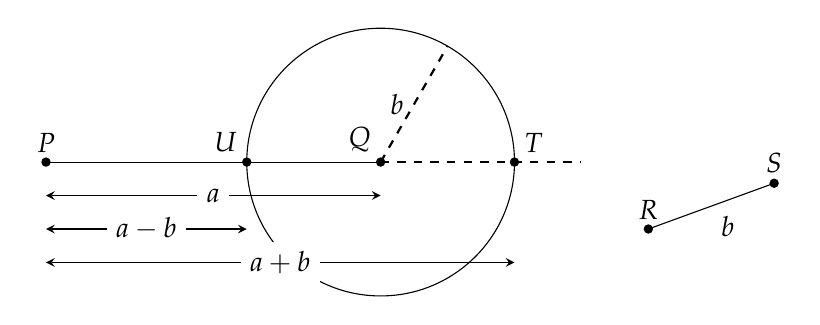
\begin{tikzpicture}[scale=.85]
\draw (0,0) -- (5,0);
\fill (0,0) node[above] {$P$} circle[radius=2pt];
\fill (5,0) node[above left] {$Q$} circle[radius=2pt];
\fill (3,0) node[above left] {$U$} circle[radius=2pt];
\fill (7,0) node[above right] {$T$} circle[radius=2pt];
\draw[thick,dashed] (5,0) -- (8,0);
\draw (5,0) circle[radius=2cm];
\draw[thick,dashed] (5,0) -- node[left] {$b$} ++(60:2cm);
\draw (9,-1) node[above] {$R$} -- node[below right] {$b$} ++(20:2cm) node[above] {$S$};
\fill (9,-1) circle[radius=2pt];
\fill (9,-1) ++(20:2cm) circle[radius=2pt];
\draw[<->] (0,-.5) -- node[fill=white] {$a$} (5,-.5);
\draw[<->] (0,-1) -- node[fill=white] {$a-b$} (3,-1);
\draw[<->] (0,-1.5) -- node[fill=white] {$a+b$} (7,-1.5);
\end{tikzpicture}
\selectlanguage{hebrew}
\end{center}

\np

\subsection*{בניית טרפז שווה שוקיים}

נבחר
$H$,
נקודה כלשהי על
$c(Q,b)$,
ונבנה את
$H'$,
השיקוף שלה סביב
$PQ$.
נסמן
$h$
האורך של
$HH'$.
\begin{center}
\selectlanguage{english}
\begin{tikzpicture}[scale=.55]
\coordinate (Q) at (0,0);
\coordinate (P) at (-6.8,0);
\coordinate (B) at (-3,-2);
\draw[thick,dashed] ($(Q)!1.3!(P)$) -- node[above,near start] {$a$} ($(P)!2.3!(Q)$);
\fill (Q) node[above left] {$Q$} circle[radius=2pt];
\fill (P) node[above] {$P$} circle[radius=2pt];
\fill (B) circle[radius=2pt];
\node[draw,circle through=(B),name path=qb] at (Q) {};
\draw[thick,dashed] (Q) -- node[left,xshift=-1pt,yshift=2pt] {$b$} (B);
\path[name path=qh] (Q) -- (-40:5cm);
\path[name path=qhp] (Q) -- (40:5cm);
\path [name intersections={of=qb and qh,by={H}}];
\path [name intersections={of=qb and qhp,by={Hp}}];
\fill[below right] (H) node[right,xshift=2pt] {$H$} circle[radius=2pt];
\fill[above right] (Hp) node[right,xshift=2pt] {$H'$} circle[radius=2pt];
\draw[thick,dashed] (H) -- node[below left,yshift=-2pt] {$h$} (Hp);
\end{tikzpicture}
\selectlanguage{hebrew}
\end{center}
נבנה את המעגלים
$c(Q,h)$, $c(H,b)$.
$K$
היא נקודת החיתוך בין המעגלים,
ן-%
$K'$
היא השיקוף של
$K$
מסביב ל-%
$PQ$.
\begin{center}
\selectlanguage{english}

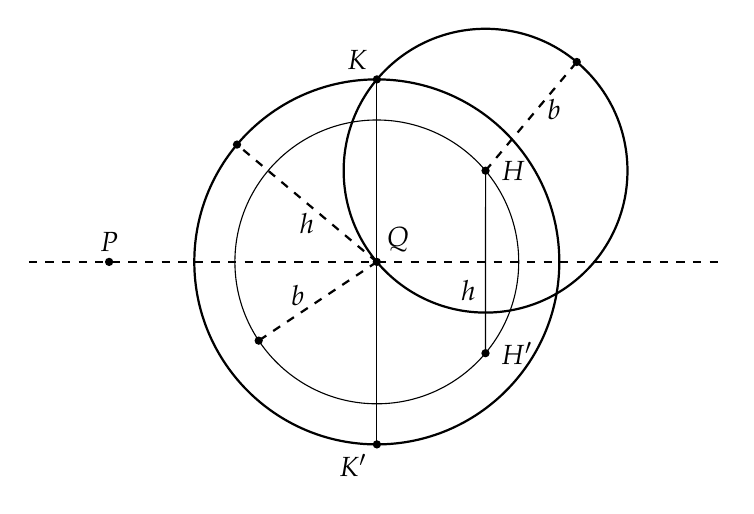
\begin{tikzpicture}[scale=.5]
\coordinate (Q) at (0,0);
\coordinate (P) at (-6.8,0);
\coordinate (B) at (-3,-2);
\draw[thick,dashed] ($(Q)!1.3!(P)$) -- ($(P)!2.3!(Q)$);
\fill (Q) node[above right] {$Q$} circle[radius=3pt];
\fill (P) node[above] {$P$} circle[radius=3pt];
\fill (B) circle[radius=3pt];
\node[draw,circle through=(B),name path=qb] at (Q) {};
\draw[thick,dashed] (Q) -- node[left,xshift=-1pt,yshift=2pt] {$b$} (B);
\path[name path=qh] (Q) -- (-40:5cm);
\path[name path=qhp] (Q) -- (40:5cm);
\path [name intersections={of=qb and qh,by={Hp}}];
\path [name intersections={of=qb and qhp,by={H}}];
\fill (H) node[right,xshift=2pt] {$H$} circle[radius=3pt];
\fill (Hp) node[right,xshift=2pt] {$H'$} circle[radius=3pt];
\draw (H) -- node[below left,yshift=-3pt] {$h$} (Hp);
\draw[thick,name path=circleqh] (Q) let
  \p1 = ($ (H) - (Hp) $),
  \n2 = {veclen(\x1,\y1)}
in
  circle (\n2)
  (Q) edge [dashed] node[below] {$h$} +(140:\n2) ++(140:\n2) coordinate (q);
\fill (q) circle[radius=3pt];
\draw[thick,name path=circlehb] (H) let
  \p1 = ($ (Q) - (B) $),
  \n2 = {veclen(\x1,\y1)}
in
  circle (\n2)
  (H) edge [dashed] node[below,near end] {$b$} +(50:\n2) ++(50:\n2)  coordinate (h);
\fill (h) circle[radius=3pt];
\path [name intersections={of=circleqh and circlehb,by={K}}];
\fill (K) node[above left] {$K$} circle[radius=3pt];
%\draw[thick] (H) -- (K);
\draw let
  \p1 = ($ (K) - (Q) $)
in
  coordinate (Kp) at (\x1,-\y1);
\fill (Kp) node[below left] {$K'$} circle[radius=3pt];
\draw (K) -- (Kp);
\end{tikzpicture}
\selectlanguage{hebrew}
\end{center}


$PQ$
הוא האנך האמצעי ל-%
$HH'$
וגם ל-%
$KK'$,
לכן שני קטעי הקו מקבילים. 
$KH = K'H' = b$
כי
$K$
נמצאת על המגעל שמרכזו 
$H$.
$K',H'$
הן שיקופים של
$K,H$.
לכן 
$KHH'K'$
הוא טרפז שווה שוקיים עם בסיסים
$KK' = 2h$, $HH'=h$.
נסמן ב-%
$d$
את אורך האלכסונים
$K'H=KH'$.


\begin{center}
\selectlanguage{english}
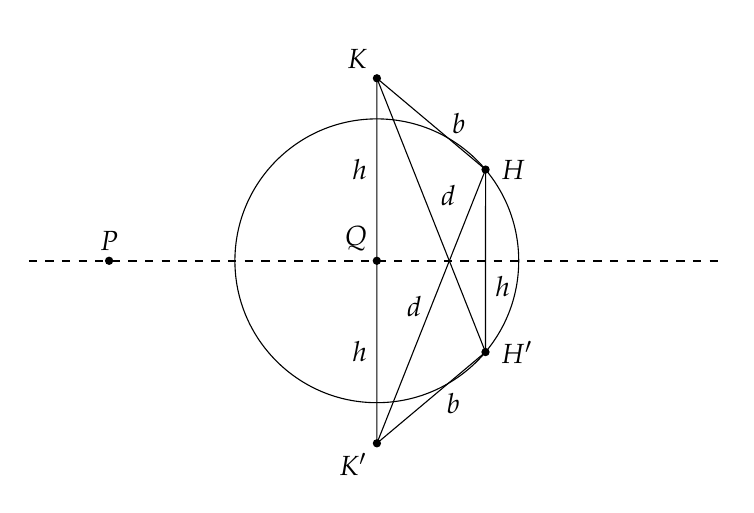
\begin{tikzpicture}[scale=.5]
\coordinate (Q) at (0,0);
\coordinate (P) at (-6.8,0);
\coordinate (B) at (-3,-2);
\draw[thick,dashed] ($(Q)!1.3!(P)$) -- ($(P)!2.3!(Q)$);
\fill (Q) node[above left] {$Q$} circle[radius=3pt];
\fill (P) node[above] {$P$} circle[radius=3pt];
%\fill (B) circle[radius=3pt];
\node[draw,circle through=(B),name path=qb] at (Q) {};
%\draw[thick,dashed] (Q) -- node[left,xshift=-1pt,yshift=2pt] {$b$} (B);
\path[name path=qh] (Q) -- (-40:5cm);
\path[name path=qhp] (Q) -- (40:5cm);
\path [name intersections={of=qb and qh,by={Hp}}];
\path [name intersections={of=qb and qhp,by={H}}];
\fill (H) node[right,xshift=2pt] {$H$} circle[radius=3pt];
\fill (Hp) node[right,xshift=2pt] {$H'$} circle[radius=3pt];
\draw (H) -- node[below right,yshift=-2pt] {$h$} (Hp);
\path[name path=circleqh] (Q) let
  \p1 = ($ (H) - (Hp) $)
in
  circle ({veclen(\x1,\y1)});
\path[name path=circlehb] (H) let
  \p1 = ($ (Q) - (B) $)
in
  circle ({veclen(\x1,\y1)});
\path [name intersections={of=circleqh and circlehb,by={K,k2}}];
\fill (K) node[above left] {$K$} circle[radius=3pt];
\draw (Q) -- node[left] {$h$} (K);
\draw (H) -- node[right,xshift=4pt] {$b$} (K);
\draw let
  \p1 = ($ (K) - (Q) $)
in
  coordinate (Kp) at (\x1,-\y1);
\fill (Kp) node[below left] {$K'$} circle[radius=3pt];
\draw (Q) -- node[left] {$h$} (Kp) -- node[right,xshift=2pt,yshift=-2pt] {$b$} (Hp);
\draw (K) -- node[above right] {$d$} (Hp);
\draw (Kp) -- node[left] {$d$} (H);
\end{tikzpicture}\label{p.ptolemy}
\end{center}

\np

\subsection*{חסימת הטרפז במעגל}
אנו רוצים להוכיח שניתן לחסום את
$KHH'K'$
במעגל. נוכיח שאם הזוויות הנגדיות של מרובע צמודות, אזי ניתן לחסום אותו במעגל, ונוכיח שבטרפז שווה שוקיים הזוויות הנגדיות צמודות. 

בספרי גיאומטריה ניתן למצוא הוכחה פשוטה לטיעון ההפוך: במרובע שניתן לחסום במעגל, הזוויות הנגדיות הן צמודות, אבל קשה למצוא הוכחה של הטיעון עצמו. לכן, אביא כאן את שתי ההוכחות.

\textbf{%
אם ניתן לחסום מרובע במעגל, הזוויות הנגדיות צמודות:%
}
ערכה של זווית היקפית הנשענת על קשת הוא מחצית ערכה של הקשת, לכן 
$\angle DAB$
היא מחצית מהקשת
$DCB$
ו-%
$\angle DCB$
היא מחצית מהקשת
$DAB$.
שתי הקשתות נשענות על כל היקף המעגל, ולכן הסכום שלהן הוא
$360^\circ$.
מכאן,
$\angle DAB + \angle DCB = \disfrac{1}{2} \cdot 360^\circ =  180^\circ$.
באופן דומה,
$\angle ADC + \angle ABC = 180^\circ$.

\vspace{-3ex}

\begin{center}
\selectlanguage{english}
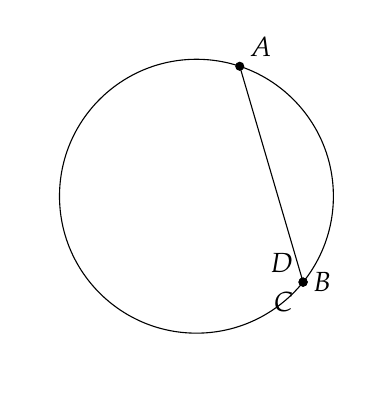
\begin{tikzpicture}[scale=.55]
\coordinate (origin) at (0,0);
\coordinate (A) at (1,3);
\node[draw,circle through=(A),name path=circle] at (origin) {};
\fill (A) node[above right] {$A$} circle[radius=3pt];
\path[name path=b] (A) -- (-50:4.5cm);
\path[name path=c] (A) -- (-120:4.5cm);
\path[name path=d] (A) -- (150:4.5cm);
\path [name intersections={of=circle and b,by={b1,B}}];
\fill (B) node[right] {$B$} circle[radius=3pt];
\path [name intersections={of=circle and c,by={c1,C}}];
\fill (C) node[below left] {$C$} circle[radius=3pt];
\path [name intersections={of=circle and d,by={d1,D}}];
\fill (D) node[above left] {$D$} circle[radius=3pt];
\draw (A) -- (B) -- (C) -- (D) -- cycle;
\end{tikzpicture}
\selectlanguage{hebrew}
\end{center}

\vspace{-3ex}

\textbf{%
מרובע שהזוויות הנגדיות שלו צמודות ניתן לחסום במעגל:%
}
ניתן לחסום כל משולש במעגל. נבנה מעגל החוסם את 
$\triangle DAB$
ונניח ש-%
$C'$
היא נקודה כך ש-%
$\angle DAB + \angle DC'B = 180^\circ$,
אבל
$C'$
\textbf{אינה}
על היקף מעגל. ללא הגבלת הכללית, נניח ש-%
$C'$
נמצאת בתוך המעגל.

\vspace{-3ex}

\begin{center}
\selectlanguage{english}
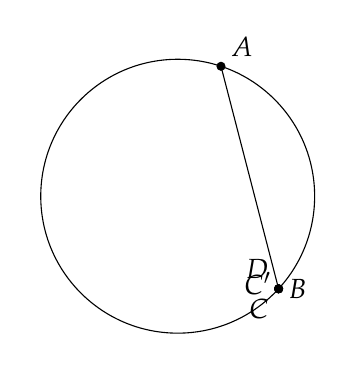
\begin{tikzpicture}[scale=.55]
\coordinate (origin) at (0,0);
\coordinate (A) at (1,3);
\node[draw,circle through=(A),name path=circle] at (origin) {};
\fill (A) node[above right] {$A$} circle[radius=3pt];
\path[name path=b] (A) -- (-50:4cm);
\path[name path=c] (A) -- (-120:4cm);
\path[name path=d] (A) -- (150:4cm);
\path [name intersections={of=circle and b,by={b1,B}}];
\fill (B) node[right] {$B$} circle[radius=3pt];
\path [name intersections={of=circle and c,by={c1,C}}];
\fill (C) node[below left] {$C$} circle[radius=3pt];
\path [name intersections={of=circle and d,by={d2,D}}];
\fill (D) node[above left] {$D$} circle[radius=3pt];
\coordinate (Cp) at ($(C)!.2!(D)$);
\draw (A) -- (B) -- (Cp) -- (D) -- cycle;
\fill (Cp) node[left,xshift=1pt,yshift=2pt] {$C'$} circle[radius=3pt];
\draw[thick,dashed] (D) -- (B) -- (C) -- (Cp);
\end{tikzpicture}
\end{center}

\vspace{-2ex}

נבנה קרן היוצאת מ-%
$DC'$
כאשר
$C$
היא נקודת החיתוך עם המעגל.  
$ABCD$
חסום מעגל ולכן:
\begin{eqnarray*}
\angle DAB + \angle DCB &=& 180^\circ\\
\angle DAB + \angle DCB &=& \angle DAB + \angle DC'B\\
\angle DCB &=& \angle DC'B\,,
\end{eqnarray*}
מצב שאינו אפשרי אם 
$C$
נמצא על המעגל ו-%
$C'$
נמצאת בתוך המעגל.

כדי להשלים את ההוכחה, נראה שהזוויות נגדיות של טרפז שווה שוקיים צמודות.
\np

\begin{center}
\selectlanguage{english}
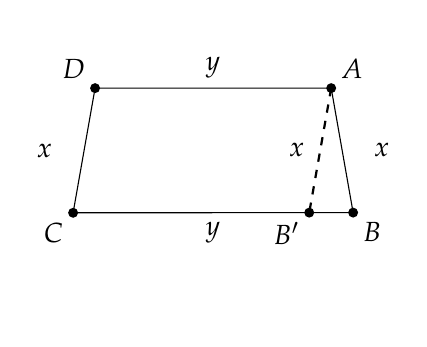
\begin{tikzpicture}[scale=.6]
\coordinate (origin) at (0,0);
\coordinate (A) at (2.5,1.8);
\node[circle through=(A),name path=circle] at (origin) {};
\fill (A) node[above right] {$A$} circle[radius=3pt];
\path[name path=b] (A) -- ++(-80:4cm);
\path[name path=d] (A) -- ++(180:6cm);
\path [name intersections={of=circle and b,by={b1,B}}];
\fill (B) node[below right] {$B$} circle[radius=3pt];
\path [name intersections={of=circle and d,by={d1,D}}];
\fill (D) node[above left] {$D$} circle[radius=3pt];
\path[name path=c] (D) -- ++(-100:4cm);
\path [name intersections={of=circle and c,by={c1,C}}];
\fill (C) node[below left] {$C$} circle[radius=3pt];
\draw (A) -- node[right,xshift=8pt] {$x$} (B);
\draw[name path=bc] (B) -- node[below] {$y$} (C);
\draw (C) -- node[left,xshift=-8pt] {$x$} (D) -- node[above] {$y$} (A);
\path[name path=para] (A) -- ++(-100:4cm);
\path [name intersections={of=para and bc,by={Bp}}];
\fill (Bp) node[below left] {$B'$} circle[radius=3pt];
\draw[thick,dashed] (A) -- node[left,xshift=-2pt] {$x$} (Bp);
\end{tikzpicture}
\selectlanguage{hebrew}
\end{center}

\vspace{-4ex}

נבנה קטע קו
$AB'$
מקביל ל-%
$CD$.
המרובע
$AB'CD$
הוא מקבילית והמשולש
$\triangle ABB'$
שווה שוקיים, כך ש-%
$\angle B= \angle ABB' = \angle AB'B=\angle C$.
באופן דומה,
$\angle A = \angle D$.
אבל הסכום של הזוויות הפנימיות של מרובע שווה ל-%
$360^\circ$:
\begin{eqnarray*}
\angle A + \angle B + \angle C + \angle D &=& 360^\circ\\
2\angle A + 2 \angle C &=& 360^\circ\\
\angle A +  \angle C &=& 180^\circ\,,
\end{eqnarray*}
ובאופן דומה
$\angle B +  \angle D = 180^\circ$.

\subsection*{משפט תלמי}

נשתמש במשפט תלמי
\L{(Ptolemy)}
שהוא משוואה הקושרת את אורכי האלכסונים ואורכי הצלעות במרובע חסום על ידי מעגל:
\[
ef = ac + bd\,.
\]

\vspace{-2ex}

\begin{center}
\selectlanguage{english}
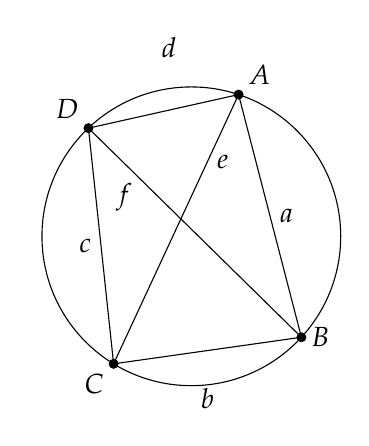
\begin{tikzpicture}[scale=.6]
\coordinate (origin) at (0,0);
\coordinate (A) at (1,3);
\node[draw,circle through=(A),name path=circle] at (origin) {};
\fill (A) node[above right] {$A$} circle[radius=3pt];
\path[name path=b] (A) -- (-50:4cm);
\path[name path=c] (A) -- (-120:4cm);
\path[name path=d] (A) -- (150:4cm);
\path [name intersections={of=circle and b,by={b1,B}}];
\fill (B) node[right] {$B$} circle[radius=3pt];
\path [name intersections={of=circle and c,by={C,c2}}];
\fill (C) node[below left] {$C$} circle[radius=3pt];
\path [name intersections={of=circle and d,by={D,d2}}];
\fill (D) node[above left] {$D$} circle[radius=3pt];
\draw (A) -- node[right] {$a$} (B) -- node[below,yshift=-10pt] {$b$} (C) -- node[left] {$c$} (D) -- node[above,xshift=2pt,yshift=16pt] {$d$}  cycle;
\draw (A) -- node[right,near start] {$e$} (C);
\draw (B) -- node[left,near end,yshift=-6pt] {$f$} (D);
\end{tikzpicture}
\selectlanguage{hebrew}

\end{center}

\vspace{-2ex}

קיימת הוכחה גיאומטרית )ראו ויקיפדיה(, אבל אני אביא הוכחה טריגונומטרית פשוטה.


מחוק הקוסינוסים עבור
$\triangle ABC$, $\triangle ADC$, $\triangle DAB$, $\triangle DCB$,
מקבלות המשוואות:
\begin{eqnarray*}
e^2 &=& a^2 + b^2 - 2ab \cos \angle B\\
e^2 &=& c^2 + d^2 - 2cd \cos \angle D\\
f^2 &=& a^2 + d^2 - 2ad \cos \angle A\\
f^2 &=& b^2 + c^2 - 2bc \cos \angle C\,.
\end{eqnarray*}

\np

הזוויות הנגדיות של מרובע חסום במעגל צמודות
$\angle C = 180^\circ - \angle A$
ו-%
$\angle D = 180^\circ - \angle B$,
ולכן:
\begin{eqnarray*}
\cos \angle D &=& - \cos \angle B\\
\cos \angle C &=& -\cos \angle A\,,
\end{eqnarray*}
וניתן להיפטר מהגורמים הטריגונומטריים. לאחר חישובים מעיקים נקבל:
\begin{eqnarray*}
e^2 &=& \frac{(ac+bd)(ad+bc)}{(ab+cd)}\\
f^2 &=& \frac{(ab+cd)(ac+bd)}{(ad+bc)}\,.
\end{eqnarray*}
נכפיל את שתי המשוואות ונפשט כדי לקבל את המשפט של תלמי:
\begin{eqnarray*}
e^2\cdot f^2 &=& (ac+bd)^2\\
ef &=& (ac+bd)\,. 
\end{eqnarray*}

\vspace{-8ex}

\subsection*{הפעלת משפט תלמי על הטרפז}

עבור הבנייה בעמוד~%
\L{\pageref{p.ptolemy}},
אורך האלכסונים הוא
$d$,
אורך השוקיים הוא
$b$,
ואורכי הבסיסים הם
$h$
ו-%
$2h$.
ממשפט תלמי:
$d\cdot d = b\cdot b + h\cdot 2h$
או
$d^2=b^2+2h^2$.

תהי
$X$
נקודה על הקו
$PQ$
המאריך את
$PQ$
ב-%
$b$.
בהמשך נבנה את 
$X$
ובינתיים נדמה לעצמנו שהיא קיימת. נגדיר 
$x = K'X$.
המשולש
$\triangle QK'X$
הוא משולש ישר זווית ולכן
$x^2 = b^2 + h^2$:


\begin{center}
\selectlanguage{english}
\begin{tikzpicture}[scale=.7]
\coordinate (Q) at (0,0);
\coordinate (P) at (-6.8,0);
\coordinate (B) at (-3,-2);
\draw[thick,dashed,name path=pq] ($(Q)!1.3!(P)$) -- ($(P)!2.3!(Q)$);
\fill (Q) node[above left] {$Q$} circle[radius=2pt];
\fill (P) node[above] {$P$} circle[radius=2pt];
%\fill (B) circle[radius=2pt];
\node[draw,circle through=(B),name path=qb] at (Q) {};
%\draw[thick,dashed] (Q) -- node[left,xshift=-1pt,yshift=2pt] {$b$} (B);
\path[name path=qh] (Q) -- (-40:5cm);
\path[name path=qhp] (Q) -- (40:5cm);
\path [name intersections={of=qb and qh,by={hp}}];
\path [name intersections={of=qb and qhp,by={H}}];
\fill (H) node[right,xshift=2pt] {$H$} circle[radius=2pt];
\fill (hp) node[right,xshift=2pt] {$H'$} circle[radius=2pt];
\draw[thick,dashed] (H) -- (hp);
\path[name path=circleqh] (Q) let
  \p1 = ($ (H) - (hp) $)
in
  circle ({veclen(\x1,\y1)});
\path[name path=circlehb] (H) let
  \p1 = ($ (Q) - (B) $)
in
  circle ({veclen(\x1,\y1)});
\path [name intersections={of=circleqh and circlehb,by={K,k2}}];
\fill (K) node[above left] {$K$} circle[radius=2pt];
\draw[thick,dashed] (Q) -- (K);
\draw[thick,dashed] (H) -- (K);
\draw[thick,dashed] let
  \p1 = ($ (K) - (Q) $)
in
  coordinate (kp) at (\x1,-\y1);
\fill (kp) node[below left] {$K'$} circle[radius=2pt];
\draw[thick,dashed] (Q) -- node[left] {$h$} (kp) -- (hp);
\draw[thick,dashed] (K) -- (hp);
\draw[thick,dashed] (kp) -- (H);
\path [name intersections={of=pq and qb,by={X,x2}}];
\fill (X) node[below right] {$X$} circle[radius=2pt];
\draw[thick,dashed] (kp) -- node[left] {$x$} (X);
\draw[very thick] (Q) -- (kp) -- (X) -- node[above,xshift=-8pt] {$b$} cycle;
\end{tikzpicture}
\selectlanguage{hebrew}

\end{center}
לפי המשפט של תלמי:
\begin{eqnarray*}
d^2 &=& b^2 + 2h^2\\
&=&(x^2-h^2)+2h^2\\
&=&x^2+h^2\,.
\end{eqnarray*}

\np

אל תחפשו משולש ישר זווית בתרשים. אנחנו טוענים 
\textbf{%
שניתן לבנות%
}
את המשולש עם צלעות
$x,h,d$.

נבנה את הנקודה
$S$
כנקודת החיתוך של המעגלים
$c(K,d)$
ו-%
$c(K',d)$:

\begin{center}
\selectlanguage{english}
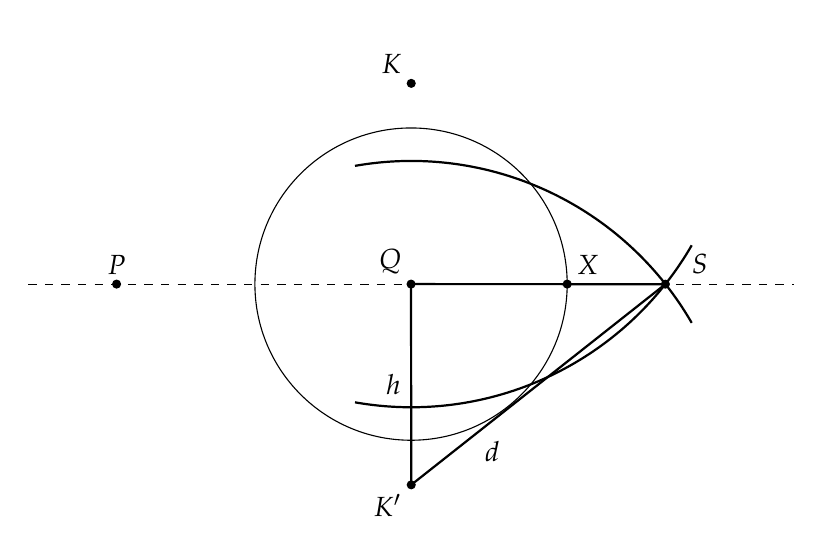
\begin{tikzpicture}[scale=.55]
\coordinate (Q) at (0,0);
\coordinate (P) at (-6.8,0);
\coordinate (B) at (-3,-2);
\draw[dashed,name path=pq] ($(Q)!1.3!(P)$) -- ($(P)!2.3!(Q)$);
\fill (Q) node[above left] {$Q$} circle[radius=3pt];
\fill (P) node[above] {$P$} circle[radius=3pt];
\node[draw,circle through=(B),name path=qb] at (Q) {};
\path[name path=qh] (Q) -- (-40:5cm);
\path[name path=qhp] (Q) -- (40:5cm);
\path [name intersections={of=qb and qh,by={Hp}}];
\path [name intersections={of=qb and qhp,by={H}}];
%\fill (H) node[right,xshift=2pt] {$H$} circle[radius=3pt];
%\fill (Hp) node[right,xshift=2pt] {$H'$} circle[radius=3pt];
\path[name path=circleqh] (Q) let
  \p1 = ($ (H) - (Hp) $)
in
  circle ({veclen(\x1,\y1)});
\path[name path=circlehb] (H) let
  \p1 = ($ (Q) - (B) $)
in
  circle ({veclen(\x1,\y1)});
\path [name intersections={of=circleqh and circlehb,by={K,k2}}];
\fill (K) node[above left] {$K$} circle[radius=3pt];
\draw[thick,dashed] let
  \p1 = ($ (K) - (Q) $)
in
  coordinate (Kp) at (\x1,-\y1);
\fill (Kp) node[below left] {$K'$} circle[radius=3pt];
\draw[thick] (Q) -- node[left] {$h$} (Kp);
\draw[thick,name path=khp] (K) let
  \p1 = ($ (H) - (Kp) $),
  \n2 = {veclen(\x1,\y1)}
in
  (K) ++(-100:\n2) arc (-100:-30:\n2);
\draw[thick,name path=kph] (Kp) let
  \p1 = ($ (H) - (Kp) $),
  \n2 = {veclen(\x1,\y1)}
in
  (Kp) ++(100:\n2) arc (100:30:\n2);
\path [name intersections={of=kph and khp,by={S}}];
\fill (S) node[above right,xshift=6pt] {$S$} circle[radius=3pt];
\draw[thick] (Kp) -- node[right,near start,yshift=-6pt] {$d$} (S);
\draw[thick] (Q) -- (S);
\path [name intersections={of=pq and qb,by={X,Xp}}];
\fill (X) node[above right] {$X$} circle[radius=3pt];
%\fill (Xp) node[above left] {$X'$} circle[radius=3pt];
%\draw (Kp) -- node[left] {$x$} (X);
%\draw (K) -- node[left] {$x$} (X);
%\fill (B) circle[radius=3pt];
%\draw[thick,dashed] (Q) -- node[left,xshift=-1pt,yshift=2pt] {$b$} (B);
\end{tikzpicture}
\end{center}
מתקבל משולש ישר זווית
$\triangle QSK'$.
לפי משפט פיתגורס
$QS^2 + h^2 = d^2$,
ולכן:
\[
QS^2 = d^2 - h^2 = x^2\,,
\]
ו-%
$QS = x$.
ניתן לבנות את הנקודה
$X$
כנקודות החיתוך בין המעגלים
$c(K,x)$
ו-%
$c(K',x)$:



\begin{center}
\selectlanguage{english}
\begin{tikzpicture}[scale=.55]
\coordinate (Q) at (0,0);
\coordinate (P) at (-6.8,0);
\coordinate (B) at (-3,-2);
\draw[dashed,name path=pq] ($(Q)!1.3!(P)$) -- ($(P)!2.3!(Q)$);
\fill (Q) node[above left] {$Q$} circle[radius=3pt];
\fill (P) node[above] {$P$} circle[radius=3pt];
\node[draw,circle through=(B),name path=qb] at (Q) {};
\path[name path=qh] (Q) -- (-40:5cm);
\path[name path=qhp] (Q) -- (40:5cm);
\path [name intersections={of=qb and qh,by={Hp}}];
\path [name intersections={of=qb and qhp,by={H}}];
%\fill (H) node[right,xshift=2pt] {$H$} circle[radius=3pt];
%\fill (Hp) node[right,xshift=2pt] {$H'$} circle[radius=3pt];
\path[name path=circleqh] (Q) let
  \p1 = ($ (H) - (Hp) $)
in
  circle ({veclen(\x1,\y1)});
\path[name path=circlehb] (H) let
  \p1 = ($ (Q) - (B) $)
in
  circle ({veclen(\x1,\y1)});
\path [name intersections={of=circleqh and circlehb,by={K,k2}}];
\fill (K) node[above left] {$K$} circle[radius=3pt];
\path[thick,dashed] let
  \p1 = ($ (K) - (Q) $)
in
  coordinate (Kp) at (\x1,-\y1);
\fill (Kp) node[below left] {$K'$} circle[radius=3pt];
%\draw[thick] (Q) -- node[left] {$h$} (Kp);
\path[name path=khp] (K) let
  \p1 = ($ (H) - (Kp) $),
  \n2 = {veclen(\x1,\y1)}
in
  (K) ++(-100:\n2) arc (-100:-30:\n2);
\path[name path=kph] (Kp) let
  \p1 = ($ (H) - (Kp) $),
  \n2 = {veclen(\x1,\y1)}
in
  (Kp) ++(100:\n2) arc (100:30:\n2);
\path [name intersections={of=kph and khp,by={S}}];
\fill (S) node[above right,xshift=6pt] {$S$} circle[radius=3pt];
%\draw[thick] (Kp) -- node[right,near start,yshift=-6pt] {$d$} (S);
%\draw[thick] (Q) -- (S);
\path [name intersections={of=pq and qb,by={X,Xp}}];
\fill (X) node[above right,xshift=8pt] {$X$} circle[radius=3pt];
\fill (Xp) node[above left] {$X'$} circle[radius=3pt];
\draw (Kp) -- node[left] {$x$} (X);
\draw (K) -- node[left] {$x$} (X);
%\fill (B) circle[radius=3pt];
%\draw[thick,dashed] (Q) -- node[left,xshift=-1pt,yshift=2pt] {$b$} (B);
\draw[name path=kx] (K) let
  \p1 = ($ (X) - (Kp) $),
  \n2 = {veclen(\x1,\y1)}
in
  (K) ++(-100:\n2) arc (-100:-30:\n2);
\draw[name path=kpx] (Kp) let
  \p1 = ($ (X) - (Kp) $),
  \n2 = {veclen(\x1,\y1)}
in
  (Kp) ++(100:\n2) arc (100:30:\n2);
\path (Xp) -- node[below] {$b$} (Q);
\path (Q) -- node[below] {$b$} (X);
\node at (-5,2) {\mbox{\boldmath $PQ=a$}};
\draw[thick,dashed] (Q) -- node[left] {$h$} (Kp);
\draw[thick,dashed] (Q) -- (X);
\end{tikzpicture}

\selectlanguage{hebrew}
\end{center}
נזכור מה אנחנו רוצים: להאריך את אורכו של
$PQ$
ב-%
$b$
או לקצר אותו ב-%
$b$.
אורכו של
$QX$
הוא
$\sqrt{x^2-h^2}=b$,
ולכן אורכו של 
$PX$
הוא 
$a+b$
ואורכו של
$PX'$
הוא
$a-b$.


%%%%%%%%%%%%%%%%%%%%%%%%%%%%%%%%%%%%%%%%%%%%%%%%%%%%%%%%%%%%%%%

\section{%
בניית קטע קו שאורכו מוגדר יחסית לשלושה קטעי קו אחרים%
}\label{s.relative}

\textbf{%
נתונים שלושה קטעי קו באורכים 
$n,m,s$.
ניתן לבנות קטע קו שאורכו
$x = \disfrac{n}{m}s$.%
}

בנה שני מעגלים משותפי מרכז:
$c_1 = c(Z,m)$
,
$c_2 = c(Z,n)$.
נבחר נקודה
$A$
כלשהי על המעגל 
$c_1$
ונבנה את המיתר
$AB$
שאורכו
$s$
ב-%
$c_1$.
)בניית המיתר עם מחוגה בלבד לפי בסעיף
\L{\ref{s.radius}}.%
(

\np

\begin{center}
\selectlanguage{english}
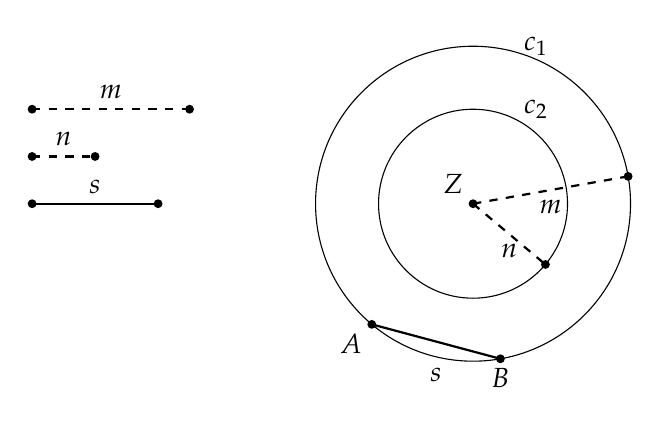
\begin{tikzpicture}[scale=.4]
\coordinate (Z) at (0,0);
\coordinate (A) at (-130:5cm);
\coordinate (B) at (-80:5cm);
\fill (Z) node[above left] {$Z$} circle[radius=4pt];
\fill (A) node[below left] {$A$} circle[radius=4pt];
\fill (B) node[below] {$B$} circle[radius=4pt];
\draw[name path=c1] (Z) circle[radius=5cm];
\draw[name path=c2] (Z) circle[radius=3cm];
\node at (2,5) {$c_1$};
\node at (2,3) {$c_2$};
\draw[thick] (A) -- node[below,yshift=-6pt] {$s$} (B);
\draw[thick,dashed] (Z) -- node[below] {$m$} ++(10:5cm);
\draw[thick,dashed] (Z) -- node[below] {$n$} ++(-40:3cm);
\fill (Z) ++ (10:5cm) circle[radius=4pt];
\fill (Z) ++ (-40:3cm) circle[radius=4pt];
\begin{scope}[xshift=-14cm,yshift=3cm]
\coordinate (m) at (0,0);
\coordinate (n) at (0,-1.5);
\coordinate (s) at (0,-3);
\coordinate (mp) at (5,0);
\coordinate (np) at (2,-1.5);
\coordinate (sp) at (4,-3);
\fill (m) circle[radius=4pt];
\fill (n) circle[radius=4pt];
\fill (s) circle[radius=4pt];
\fill (mp) circle[radius=4pt];
\fill (np) circle[radius=4pt];
\fill (sp) circle[radius=4pt];
\draw[thick,dashed] (m) -- node[above] {$m$} (mp);
\draw[thick,dashed] (n) -- node[above] {$n$} (np);
\draw[thick] (s) -- node[above] {$s$} (sp);
\end{scope}
\end{tikzpicture}
\selectlanguage{hebrew}
\end{center}

נניח ש-%
$m>n$,
אחרת נחליף את הסימונים של
$m,n$.


נניח גם שהמיתר 
$s$
אינו חותך את
$c_2$.
אם לא, נשתמש בבנייה של סעיף
\L{\ref{s.add-subtract}}
כדי להכפיל את
$m,n$
במספר שלם
$k$
עד שהמיתר לא חותך. שימו לב שהכפלת הערכים אינה משנה את הערך שאנחנו בונים
$x = \disfrac{kn}{km}s = \disfrac{n}{m}s$.


נבחר נקודה כלשהי
$H$
על המעגל
$c_2$.
נסמן את אורך הקטע
$AH$
ב-%
$w$.
נבנה נקודה
$K$
על 
$c_2$
כך שאורך הקטע
$BK$
גם הוא
$w$.



\begin{center}
\selectlanguage{english}
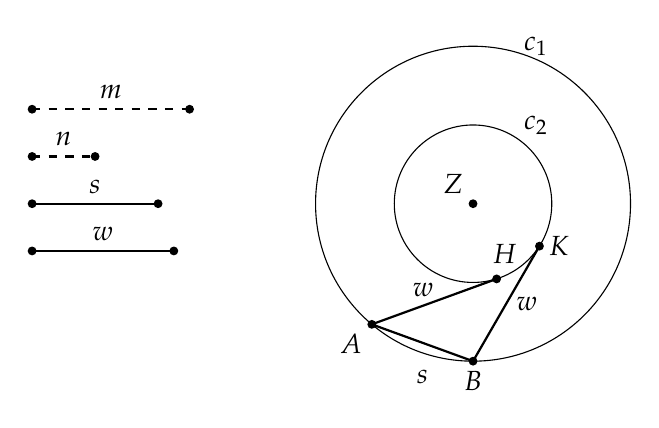
\begin{tikzpicture}[scale=.4]
\coordinate (Z) at (0,0);
\coordinate (A) at (-130:5cm);
\coordinate (B) at (-90:5cm);
\fill (Z) node[above left] {$Z$} circle[radius=4pt];
\fill (A) node[below left] {$A$} circle[radius=4pt];
\fill (B) node[below] {$B$} circle[radius=4pt];
\draw[name path=c1] (Z) circle[radius=5cm];
\draw[name path=c2] (Z) circle[radius=2.5cm];
\node at (2,5) {$c_1$};
\node at (2,2.5) {$c_2$};
\draw[thick] (A) -- node[below,yshift=-6pt] {$s$} (B);
\draw[thick] (A) -- node[above,xshift=-4pt,yshift=-2pt] {$w$} +(20:120pt) coordinate (H);
\fill (H) node[above right,xshift=-5pt,yshift=2pt] {$H$} circle[radius=4pt];
\draw[thick] (B) -- node[right] {$w$} +(60:120pt) coordinate (K);
\fill (K) node[right] {$K$} circle[radius=4pt];
\begin{scope}[xshift=-14cm,yshift=3cm]
\coordinate (m) at (0,0);
\coordinate (n) at (0,-1.5);
\coordinate (s) at (0,-3);
\coordinate (w) at (0,-4.5);
\coordinate (mp) at (5,0);
\coordinate (np) at (2,-1.5);
\coordinate (sp) at (4,-3);
\coordinate (wp) at (4.5,-4.5);
\fill (m) circle[radius=4pt];
\fill (n) circle[radius=4pt];
\fill (s) circle[radius=4pt];
\fill (w) circle[radius=4pt];
\fill (mp) circle[radius=4pt];
\fill (np) circle[radius=4pt];
\fill (sp) circle[radius=4pt];
\fill (wp) circle[radius=4pt];
\draw[thick,dashed] (m) -- node[above] {$m$} (mp);
\draw[thick,dashed] (n) -- node[above] {$n$} (np);
\draw[thick] (s) -- node[above] {$s$} (sp);
\draw[thick] (w) -- node[above] {$w$} (wp);
\end{scope}
\end{tikzpicture}
\end{center}

%\vspace{-2ex}

$\triangle AHZ$, $\triangle BZK$
חופפים לפי צ.צ.צ.: 
$ZA=ZB=m$
הרדיוס של מעגל
$c_1$,
$ZH=ZK=n$
הרדיוס של המעגל
$c_2$,
ו-%
$AH=BK=w$
לפי הבנייה.

\vspace{-1ex}

\begin{center}
\selectlanguage{english}
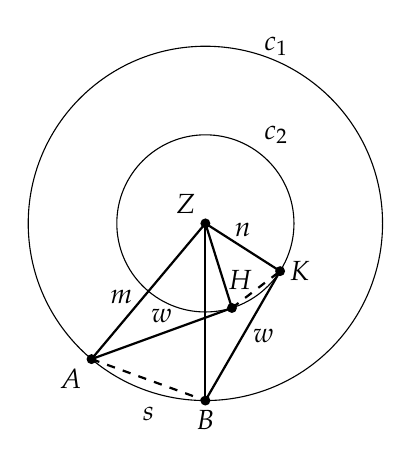
\begin{tikzpicture}[scale=.45]
\coordinate (Z) at (0,0);
\coordinate (A) at (-130:5cm);
\coordinate (B) at (-90:5cm);
\fill (Z) node[above left] {$Z$} circle[radius=4pt];
\fill (A) node[below left] {$A$} circle[radius=4pt];
\fill (B) node[below] {$B$} circle[radius=4pt];
\draw[name path=c1] (Z) circle[radius=5cm];
\draw[name path=c2] (Z) circle[radius=2.5cm];
\node at (2,5) {$c_1$};
\node at (2,2.5) {$c_2$};
\draw[thick,dashed] (A) -- node[below,yshift=-6pt] {$s$} (B);
\draw[thick] (A) -- node[above] {$w$} +(20:120pt) coordinate (H);
\fill (H) node[above right,xshift=-5pt,yshift=3pt] {$H$} circle[radius=4pt];
\draw[thick] (B) -- node[right] {$w$} +(60:120pt) coordinate (K);
\fill (K) node[right] {$K$} circle[radius=4pt];
\draw[thick] (Z) -- node[left,xshift=-2pt,yshift=-2pt] {$m$} (A);
\draw[thick] (Z) -- (B);
\draw[thick] (Z) -- (H);
\draw[thick] (Z) -- node[above] {$n$} (K);
\draw[thick,dashed] (H) -- (K);
\end{tikzpicture}
\selectlanguage{hebrew}
\end{center}

\vspace{-3ex}

מ-%
$\triangle AZH \cong \triangle BZK$,
אנו מקבלים
$\angle AZB = \angle HZK$.
קצת קשה לראות את השוויונות האלה בתרשים, אבל התרשים שלהלן מבהיר את היחסים בין הזוויות. נגדיר
$\alpha = \angle AZH = \angle BZK$
ו-%
$\beta = \angle BZH$,
וקל לראות ש-%
$\angle AZB = \angle HZK = \alpha - \beta$.
\begin{center}

\np

\selectlanguage{english}
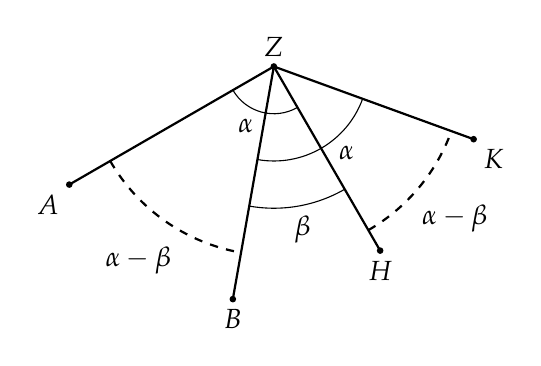
\begin{tikzpicture}[scale=.6]
\coordinate (Z) at (0,0);
\coordinate (A) at (-150:5cm);
\coordinate (B) at (-100:5cm);
\coordinate (H) at (-60:4.5cm);
\coordinate (K) at (-20:4.5cm);
\fill (Z) circle[radius=2pt];
\fill (A) circle[radius=2pt];
\fill (B) circle[radius=2pt];
\fill (H) circle[radius=2pt];
\fill (K) circle[radius=2pt];
\draw[thick] (A) node[below left] {$A$} -- (Z) node[above] {$Z$} -- (B) node[below] {$B$};
\draw[thick] (H) node[below] {$H$} -- (Z) -- (K) node[below right] {$K$};
\draw (-150:1cm) arc (-150:-60:1);
\draw (-100:2cm) arc (-100:-20:2);
\draw (-100:3cm) arc (-100:-60:3);
\draw[thick,dashed] (-150:4cm) arc (-150:-100:4);
\draw[thick,dashed] (-60:4cm) arc (-60:-20:4);
\node at (-115:1.4) {$\alpha$};
\node at (-50:2.4) {$\alpha$};
\node at (-80:3.5) {$\beta$};
\node at (-40:5) {$\alpha - \beta$};
\node at (-125:5) {$\alpha - \beta$};
\end{tikzpicture}
\selectlanguage{hebrew}
\end{center}

\vspace{-1ex}

זוויות הקודקוד של שני משולשים שווי שוקיים שוות, ולכן
$\triangle AZB\sim\triangle HZK$.

\vspace{-1ex}

\begin{center}
\selectlanguage{english}
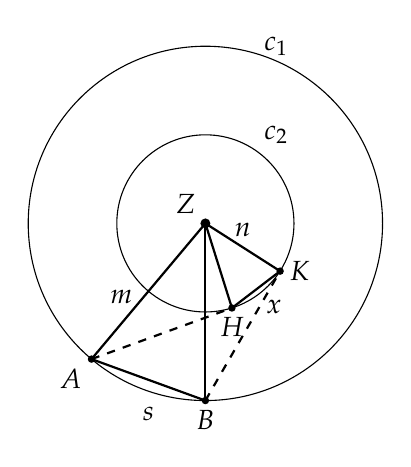
\begin{tikzpicture}[scale=.45]
\coordinate (Z) at (0,0);
\coordinate (A) at (-130:5cm);
\coordinate (B) at (-90:5cm);
\fill (Z) node[above left] {$Z$} circle[radius=4pt];
\fill (A) node[below left] {$A$} circle[radius=3pt];
\fill (B) node[below] {$B$} circle[radius=3pt];
\draw[name path=c1] (Z) circle[radius=5cm];
\draw[name path=c2] (Z) circle[radius=2.5cm];
\node at (2,5) {$c_1$};
\node at (2,2.5) {$c_2$};
\draw[thick] (A) -- node[below,yshift=-6pt] {$s$} (B);
\path[thick,dashed] (A) -- +(20:120pt) coordinate (H);
\fill (H) node[below] {$H$} circle[radius=3pt];
\path[thick,dashed] (B) -- +(60:120pt) coordinate (K);
\fill (K) node[right] {$K$} circle[radius=3pt];
\draw[thick] (Z) -- node[left,xshift=-2pt,yshift=-2pt] {$m$} (A);
\draw[thick] (Z) -- (B);
\draw[thick] (Z) -- (H);
\draw[thick] (Z) -- node[above] {$n$} (K);
\draw[thick] (H) -- node[below right] {$x$} (K);
\draw[thick,dashed] (A) -- (H);
\draw[thick,dashed] (B) -- (K);
\end{tikzpicture}
\selectlanguage{hebrew}
\end{center}

\vspace{-2ex}
נסמן את קטע הקו
$HK$
ב-%
$x$,
ונקבל:
\begin{eqnarray*}
\frac{m}{s} &=& \frac{n}{x}\\
x&=&\frac{n}{m}s\,.
\end{eqnarray*}

\vspace{-5ex}

%%%%%%%%%%%%%%%%%%%%%%%%%%%%%%%%%%%%%%%%%%%%%%%%%%%%%%%%%%%%%%%

\section{%
מציאת נקודת החיתוך של שני קווים%
}\label{s.two-lines}

\textbf{%
נתונים שני קווים המכילים את קטעי הקו
$AB,CD$.
ניתן לבנות את נקודת החיתוך שלהם עם מחוגה בלבד.%
}

נבנה את הנקודה
$C'$
כשיקוף של
$C$
מסביב ל-%
$AB$,
ו-%
$D'$
כשיקוף של
$D$
מסביב לקו
$AB$.

נקודת החיתוך
$S$
נמצאת על הקו
$AB$,
כי
$\triangle CZS\cong \triangle C'ZS$
לפי צ.ז.צ., כי
$CZ=C'Z$,
$\angle CZS = \angle C'ZS = 90^\circ$
ו-%
$ZS$
צלע משותף. מכאן ש-%
$C'S=CS$,
ובאופן דומה
$D'S=DS$.


\begin{center}
\selectlanguage{english}
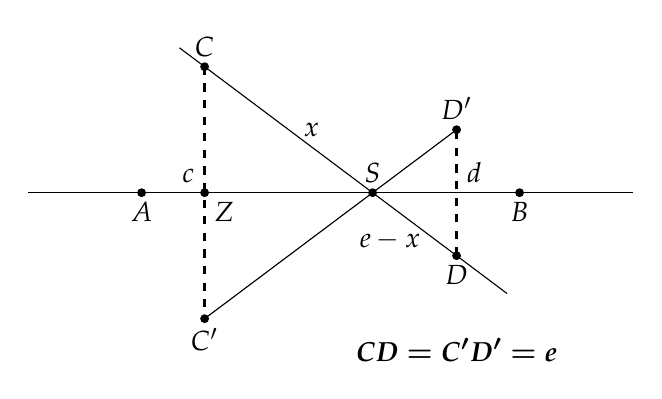
\begin{tikzpicture}[scale=.8]
\coordinate (A) at (-4,0);
\coordinate (B) at (2,0);
\coordinate (C) at (-3,2);
\coordinate (D) at (1,-1);
\coordinate (Cp) at (-3,-2);
\coordinate (Dp) at (1,1);
\fill (A) node[below] {$A$} circle[radius=2pt];
\fill (B) node[below] {$B$} circle[radius=2pt];
\fill (C) node[above] {$C$} circle[radius=2pt];
\fill (D) node[below] {$D$} circle[radius=2pt];
\fill (Cp) node[below] {$C'$} circle[radius=2pt];
\fill (Dp) node[above] {$D'$} circle[radius=2pt];
\draw[name path=ab] ($(A)!1.3!(B)$) -- ($(B)!1.3!(A)$);
\draw[name path=cd] ($(C)!1.2!(D)$) -- ($(D)!1.1!(C)$);
\path [name intersections={of=ab and cd,by={S}}];
\fill (S) node[above] {$S$} circle[radius=2pt];
\draw (Cp) -- (Dp);
\draw[thick,dashed] (C) -- node[above left] {$c$} (Cp);
\draw[thick,dashed] (D) -- node[above right] {$d$} (Dp);
\path (C) -- node[right,xshift=2pt] {$x$} (S);
\path (S) -- node[left,near end,xshift=-2pt] {$e-x$} (D);
\node at (1,-2.5) {\mbox{\boldmath $CD=C'D'=e$}};
\fill (-3,0) node[below right] {$Z$} circle[radius=2pt];
\end{tikzpicture}
\selectlanguage{hebrew}
\end{center}

\np

נסמן
$x = CS, c = CC', d = DD', e = CD$.
$\triangle CSC'\sim\triangle DSD'$
ולכן
$\disfrac{x}{e-x} = \disfrac{c}{d}$.
נפתור את המשוואה עבור
$x$
ונקבל
$x=\disfrac{c}{c+d}e$.

אם
$C,D$
נמצאות באותו צד של
$AB$:

\begin{center}
\selectlanguage{english}
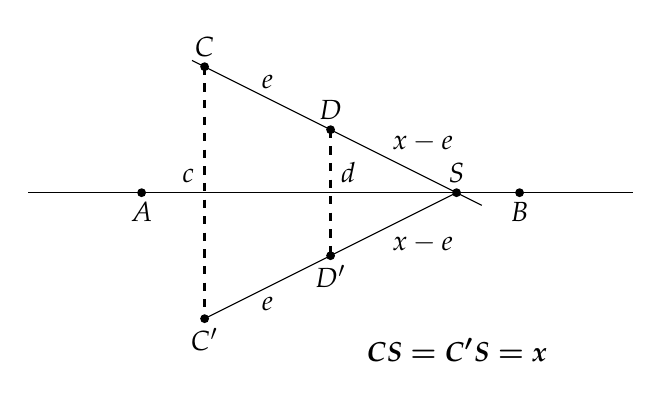
\begin{tikzpicture}[scale=.8]
\coordinate (A) at (-4,0);
\coordinate (B) at (2,0);
\coordinate (C) at (-3,2);
\coordinate (D) at (-1,1);
\coordinate (Cp) at (-3,-2);
\coordinate (Dp) at (-1,-1);
\fill (A) node[below] {$A$} circle[radius=2pt];
\fill (B) node[below] {$B$} circle[radius=2pt];
\fill (C) node[above] {$C$} circle[radius=2pt];
\fill (D) node[above] {$D$} circle[radius=2pt];
\fill (Cp) node[below] {$C'$} circle[radius=2pt];
\fill (Dp) node[below] {$D'$} circle[radius=2pt];
\draw[name path=ab] ($(A)!1.3!(B)$) -- ($(B)!1.3!(A)$);
\draw[name path=cd] ($(C)!2.2!(D)$) -- ($(D)!1.1!(C)$);
\path [name intersections={of=ab and cd,by={S}}];
\fill (S) node[above] {$S$} circle[radius=2pt];
\draw (Cp) -- (S);
\draw[thick,dashed] (C) -- node[above left] {$c$} (Cp);
\draw[thick,dashed] (D) -- node[above right] {$d$} (Dp);
\path (C) -- node[above] {$e$} (D);
\path (Cp) -- node[below] {$e$} (Dp);
\path (D) -- node[above right,xshift=-4pt] {$x-e$} (S);
\path (Dp) -- node[below right,xshift=-4pt] {$x-e$} (S);
\node at (1,-2.5) {\mbox{\boldmath $CS=C'S=x$}};
\end{tikzpicture}
\selectlanguage{hebrew}
\end{center}

$\triangle CSC'\sim\triangle DSD'$,
ולכן
$\disfrac{x}{x-e}=\disfrac{c}{d}$.
נפתור עבור
$x$
ונקבל
$x=\disfrac{c}{c-d}e$.

\smallskip

נבנה את המעגלים
$c(C',d)$
,
$c(D,e)$,
ונסמן נקודת החיתוך שלהם ב-%
$H$.
סכום האורכים של שני הקטעים
$CC',C'H$
הוא
$c + d$.
יש להראות ש-%
$H$
נמצאת בהמשך הקו של
$CC'$
ואז אורך הקטע
$CH$
יהיה
$c+d$.
)במקרה ש-%
$D$
נמצאת על אותו צד של
$AB$
ש-%
$C$
נמצאת, 
$CH = c - d$.(
\begin{center}

\selectlanguage{english}
\begin{tikzpicture}[scale=.8]
\coordinate (A) at (-4,0);
\coordinate (B) at (2,0);
\coordinate (C) at (-3,2);
\coordinate (D) at (1,-1);
\coordinate (Cp) at (-3,-2);
\coordinate (Dp) at (1,1);
\fill (A) node[below left] {$A$} circle[radius=2pt];
\fill (B) node[below] {$B$} circle[radius=2pt];
\fill (C) node[above] {$C$} circle[radius=2pt];
\fill (D) node[below] {$D$} circle[radius=2pt];
\fill (Cp) node[left] {$C'$} circle[radius=2pt];
\fill (Dp) node[above] {$D'$} circle[radius=2pt];
\draw[name path=ab] ($(A)!1.3!(B)$) -- ($(B)!1.3!(A)$);
\draw[name path=cd] ($(C)!1.2!(D)$) -- ($(D)!1.1!(C)$);
\path [name intersections={of=ab and cd,by={S}}];
\fill (S) node[above,yshift=4pt] {$S$} circle[radius=2pt];
\draw (Cp) -- node[below right] {$e$} (Dp);
\path (C) -- node[above left] {$c$} (Cp);
\draw[thick,dashed] (D) -- node[above right] {$d$} (Dp);
\node at (3.5,-3) {\mbox{\boldmath $CD=C'D'=DH=e$}};
\draw[name path=circled] (D) let
  \p1 = ($ (D) - (C) $),
  \n2 = {veclen(\x1,\y1)}
in
  ++(130:\n2) arc (130:230:\n2);

\draw[name path=circlecp] (Cp) let
  \p1 = ($ (D) - (Dp) $),
  \n2 = {veclen(\x1,\y1)}
in
  ++(-180:\n2) arc (-180:0:\n2);
\path [name intersections={of=circled and circlecp,by={H}}];
\fill (H) node[below left] {$H$} circle[radius=2pt];
\draw[thick,dashed] ($(C)!1.2!(H)$) -- (C);
\draw (H) -- node[right] {$d$} (Cp);
\draw (D) -- node[right,xshift=14pt,yshift=8pt] {$e$} (H);
\end{tikzpicture}

\selectlanguage{hebrew}
\end{center}
מההגדרה של
$H$
כחיתוך של המעגלים
$c(C',d)$,
$c(D,e)$,
אנו מקבלים
$C'H=d$
,
$DH=e$.
אבל 
$C'D'=e, DD'=e$,
ולכן המרובע
$C'D'DH$
הוא מקבילית, כי האורכים של זוגות הצלעות הנגדיות שוות. לפי הבנייה, קטע הקו
$DD'$
מקביל ל-%
$CC'$,
ולכן
$C'H$
שמקביל ל-%
$DD'$
מקביל גם ל-%
$CC'$.
אחת מנקודות הקצה של הקטע היא
$C'$,
והקטע חייב להיות על ההמשך של הקטע
$CC'$.

האורכים
$c,d,e$
נתונים והוכחנו בסעיף
\L{\ref{s.add-subtract}}
שניתן לבנות קטע באורך
$c+d$,
ובסעיף
\L{\ref{s.relative}}
הוכחנו שניתן לבנות קטע באורך
$x=\disfrac{c}{c+d}e$.
$S$
היא נקודת החיתוך של המעגלים
$c(C,x)$
ו-%
$c(C',x)$.

\np

\begin{center}
\selectlanguage{english}
\begin{tikzpicture}[scale=.8]
\coordinate (A) at (-4,0);
\coordinate (B) at (2,0);
\coordinate (C) at (-3,2);
\coordinate (D) at (1,-1);
\coordinate (Cp) at (-3,-2);
\coordinate (Dp) at (1,1);
\fill (A) node[below left] {$A$} circle[radius=2pt];
\fill (B) node[below] {$B$} circle[radius=2pt];
\fill (C) node[above] {$C$} circle[radius=2pt];
\fill (D) node[below] {$D$} circle[radius=2pt];
\fill (Cp) node[left] {$C'$} circle[radius=2pt];
\fill (Dp) node[above] {$D'$} circle[radius=2pt];
\draw[name path=ab] ($(A)!1.3!(B)$) -- ($(B)!1.3!(A)$);
\draw[name path=cd] ($(C)!1.2!(D)$) -- ($(D)!1.1!(C)$);
\path [name intersections={of=ab and cd,by={S}}];
\fill (S) node[above,yshift=4pt] {$S$} circle[radius=2pt];
\draw (Cp) -- (Dp);
\path (C) -- node[above,yshift=4pt] {$x$} (S);
\path (Cp) -- node[below,yshift=-4pt] {$x$} (S);
\path (C) -- node[above left] {$c$} (Cp);
\draw[thick,dashed] (D) -- node[above right] {$d$} (Dp);
\node at (3,-3) {\mbox{\boldmath $CD=C'D'=DH=e$}};
\draw[name path=circled] (C) let
  \p1 = ($ (S) - (C) $),
  \n2 = {veclen(\x1,\y1)}
in
  ++(-10:\n2) arc (-10:-100:\n2);

\draw[name path=circlecp] (Cp) let
  \p1 = ($ (S) - (C) $),
  \n2 = {veclen(\x1,\y1)}
in
  ++(100:\n2) arc (100:0:\n2);
\draw[thick,dashed] (Cp) -- (C);
\end{tikzpicture}
\end{center}


%%%%%%%%%%%%%%%%%%%%%%%%%%%%%%%%%%%%%%%%%%%%%%%%%%%%%%%%%%%%%%%

\section{%
מציאת נקודת החיתוך של קו עם מעגל
}\label{s.line-circle}

\textbf{%
נתון מעגל
$k=C(M,r)$
וקו
$AB$.
ניתן לבנות את נקודות החיתוך שלהם עם מחוגה בלבד.%
}

נבנה את 
$M'$,
השיקוף של
$M$
מסביב ל-%
$AB$,
והמעגל
$k'=c(M',r)$.
נקודות החיתוך של המעגלים
$k,k'$
הן נקודות החיתוך של הקו 
$AB$
והמעגל
$k$.
\begin{center}

\selectlanguage{english}
\begin{tikzpicture}[scale=.5]
\coordinate (A) at (-7,0);
\coordinate (B) at (8,0);
\coordinate (M) at (0,-2);
\coordinate (Mp) at (0,2);
\fill (A) node[below] {$A$} circle[radius=3pt];
\fill (B) node[below] {$B$} circle[radius=3pt];
\fill (M) node[below left] {$M$} circle[radius=3pt];
\fill (Mp) node[above left] {$M'$} circle[radius=2pt];
\draw[name path=c1] (M) circle[radius=3cm];
\draw[name path=c2] (Mp) circle[radius=3cm];
\draw[name path=ab] ($(A)!1.2!(B)$) -- ($(B)!1.2!(A)$);
\path [name intersections={of=c1 and c2,by={S1,S2}}];
\fill (S1) circle[radius=3pt];
\fill (S2) circle[radius=3pt];
\path[name path=radius1] (M) -- ++(15:4cm);
\path [name intersections={of=c1 and radius1,by={R1}}];
\draw[thick,dashed] (M) -- node[below] {$r$} (R1);
\path[name path=radius2] (Mp) -- ++(40:4cm);
\path [name intersections={of=c2 and radius2,by={R2}}];
\draw[thick,dashed] (Mp) -- node[above] {$r$} (R2);
\fill (R1) circle[radius=3pt];
\fill (R2) circle[radius=3pt];
\end{tikzpicture}
\selectlanguage{hebrew}

\end{center}
בנייה זו אינה אפשרית אם מרכז המעגל
$M$
נמצא על הקו
$AB$.
במקרה זה, יש להאריך ולקצר את הקטע
$AM$
באורך 
$r$
לפי הבנייה המתוארת בסעיף~
\L{\ref{s.add-subtract}}.
נקודות הקצה של הקטעים האלה הן נקודות החיתוך של
$k$
עם
$AB$.
\begin{center}

\selectlanguage{english}
\begin{tikzpicture}[scale=.5]
\coordinate (A) at (-7,0);
\coordinate (B) at (8,0);
\coordinate (M) at (0,0);
\fill (A) node[below] {$A$} circle[radius=3pt];
\fill (B) node[below] {$B$} circle[radius=3pt];
\fill (M) node[below left] {$M$} circle[radius=3pt];
\draw[name path=c1] (M) circle[radius=3cm];
\draw[name path=ab] ($(A)!1.2!(B)$) -- ($(B)!1.2!(A)$);
\path[name path=radius1] (M) -- ++(-30:4cm);
\path [name intersections={of=c1 and radius1,by={R1}}];
\draw[thick,dashed] (M) -- node[below] {$r$} (R1);
\path [name intersections={of=c1 and ab,by={S1,S2}}];
\fill (S1) node[above right] {$AM+r$} circle[radius=3pt];
\fill (S2) node[above left] {$AM-r$} circle[radius=3pt];
\fill (R1) circle[radius=3pt];
\end{tikzpicture}
\end{center}

\selectlanguage{english}


\tikzsetfigurename{straightedge-only}
% !TeX root = construct.tex

\selectlanguage{hebrew}

\chapter{אני מסתפק בסרגל )ועוד משהו(}

%%%%%%%%%%%%%%%%%%%%%%%%%%%%%%%%%%%%%%%%%%%%%%%%%%%%%%%%%%%%%%%


האם כל בנייה בסרגל ומחוגה ניתנת לבנייה עם סרגל בלבד? התשובה היא שלילית. ב-%
$1822$
המתיטיקאי הצרפתי
\L{Jean-Victor Poncelet}
שיער שכן ניתן להסתפק בסרגל בלבד, בתנאי שקיים במישור מעגל
\textbf{%
אחד%
}.
המשפט הוכח ב-
$1833$
על ידי המתימטיקאי השוויצרי
\L{Jakob Steiner}.
בפרק זה אביא את הוכחת המשפט המבוססת על ההוכחה שמופיעה כבעייה
$34$
ב-%
\L{\cite{dorrie1}},
ועובדה על ידי
\L{Michael Woltermann} \L{\cite{dorrie2}}.%
\footnote{%
ברצוני להודות לו על הרשות להתשמש בעבודתו.
}

%%%%%%%%%%%%%%%%%%%%%%%%%%%%%%%%%%%%%%%%%%%%%%%%%%%%%%%%%%%%%%%


כל צעד בבנייה על סרגל ומחוגה הוא אחת משלושת פעולות האלו:
\begin{itemize}
\setlength{\itemsep}{0pt}
\item
מציאת נקודת החיתוך של שני קווים ישרים.
\item
מציאת נקודות החיתוך של קו ישר עם מעגל.
\item
מציאת נקודות החיתוך של שני מעגלים.
\end{itemize}
ברור שניתן לבצע את הפעולה הראשונה עם סרגל בלבד. עלינו להראות שעבור שתי הפעולות האחרות ניתן למוצא בנייה שקולה המשתמשת רק בסרגל עם מעגל אחד.

%%%%%%%%%%%%%%%%%%%%%%%%%%%%%%%%%%%%%%%%%%%%%%%%%%%%%%%%%%%%%%%

מה המשמעות של בנייה עם סרגל בלבד? מעגל מוגדר על ידי נקודה
$O$,
שהיא מרכז המעגל, וקטע קו באורך
$r$,
הרדיוס, שאחת מהנקודות הקצה שלה היא
$O$.
אם נצליח לבנות את הנקודות
$X,Y$
המסומנות בהתרשים שלהלן, נוכל לטעון שהצלחנו לבנות את נקודות החיתוך של מעגל נתון עם קו נתון ושל שני מעגלים נתונים. המעגלים המצויירים בקו מקווקוו לא ממש מפיעים בבנייה. בהמשך, המעגל היחיד הנתון יצוייר בקו רגיל, ומעגלים המשמשים רק להדגמת הבנייה והוכחתה יהיו מקווקווים.


\begin{center}
\selectlanguage{english}
\begin{tikzpicture}[scale=.9]
\fill (0,0) node[above right] {$O$} circle[radius=1.5pt];
\draw[thick,dashed,name path=circle] (0,0) circle[radius=2cm];
\draw (0,0) -- node[left] {$r$} ++(-60:2cm);
\fill (0,0) ++(-60:2cm) circle[radius=1.5pt];
\draw[name path=line] (-3,-.5) -- ++(20:6cm);
\path [name intersections={of=circle and line,by={X,Y}}];
\fill (X) node[above right,xshift=-2pt,yshift=4pt] {$X$} circle[radius=1.5pt];
\fill (Y) node[above left] {$Y$} circle[radius=1.5pt];
\begin{scope}[xshift=6cm]
\fill (0,0) node[above right] {$O_1$} circle[radius=1.5pt];
\fill (3,0) node[above right] {$O_2$} circle[radius=1.5pt];
\draw[thick,dashed,name path=circle1] (0,0) circle[radius=2cm];
\draw[thick,dashed,name path=circle2] (3,0) circle[radius=2cm];
\draw (0,0) -- node[left] {$r_1$} ++(-70:2cm);
\draw (3,0) -- node[left,below] {$r_2$} ++(-20:2cm);
\fill (0,0) ++(-70:2cm) circle[radius=1.5pt];
\fill (3,0) ++(-20:2cm) circle[radius=1.5pt];
\path [name intersections={of=circle1 and circle2,by={X,Y}}];
\fill (X) node[above,yshift=4pt] {$X$} circle[radius=1.5pt];
\fill (Y) node[below,yshift=-4pt] {$Y$} circle[radius=1.5pt];
\end{scope}
\end{tikzpicture}
\selectlanguage{hebrew}
\end{center}


%%%%%%%%%%%%%%%%%%%%%%%%%%%%%%%%%%%%%%%%%%%%%%%%%%%%%%%%%%%%%%%


תחילה נביא חמש בניות עזר נחוצות )סעיפים
\L{\ref{s.parallel}--\ref{s.root}}%
(,
ואחר כך נראה איך למצוא נקודות חיתוך של קו עם מעגל )סעיף
\L{\ref{s.line-circle-straight}}%
( ושל שני מעלגים )סעיף
\L{\ref{s.circle-circle}}%
(.


%%%%%%%%%%%%%%%%%%%%%%%%%%%%%%%%%%%%%%%%%%%%%%%%%%%%%%%%%%%%%%%

\section{%
בניית קו המקביל לקו נתון%
}\label{s.parallel}

\textbf{%
נתון קו
$l$
המוגדר על ידי שתי נקודות
$A,B$,
ונקודה 
$P$
)שאיננה על הקו(, ניתן לבנות קו דרך
$P$
המקביל ל-%
$AB$.%
}

נפריד את הבנייה לשני מקרים:

\np

\begin{itemize}
\item
"קו מכוון": נתונה הנקודה 
$M$
\textbf{%
החוצה
}
את
$AB$.
\item
כל קו אחר.
\end{itemize}

\vspace{-2ex}

\textbf{%
מקרה ראשון, קו מכוון:
}
נבנה קרן הממשיכה את
$AP$,
ונבחר
$S$,
נקודה כלשהי על הקרן מעבר ל-%
$P$.
נבנה את הקווים
$SB$, $SM$, $BP$.
נסמן ב-%
$O$
את נקודת החיתוך של 
$BP$
עם
$SM$.
נבנה קרן הממשיכה את
$AO$
ונסמן ב-%
$Q$
את החיתוך של הקרן
$AO$
עם
$SB$.
\begin{center}
\selectlanguage{english}
\vspace*{-4pt}
\begin{tikzpicture}
\draw[name path=pq] (-4,0) -- (4,0);
\draw (-2,-2) node[below left] {$A$} coordinate (A) -- (2,-2) node[below right] {$B$} coordinate (B);
\fill (A) circle[radius=1.5pt];
\fill (B) circle[radius=1.5pt];
\draw[name path=as] (A) -- ++(50:4cm) node[above] {$S$} coordinate (S);
\fill (S) circle[radius=1.5pt];
\draw[name path=sb] (S) -- (B);
\path [name intersections={of=pq and as,by={P}}];
\path [name intersections={of=pq and sb,by={Q}}];
\fill (P) node[above left] {$P$} circle[radius=1.5pt];
\fill (Q) node[above right] {$Q$} circle[radius=1.5pt];
\draw[name path=pb] (P) -- (B);
\draw[name path=qa] (Q) -- (A);
\path [name intersections={of=pb and qa,by={O}}];
\fill (O) node[right,xshift=2pt] {$O$} circle[radius=1.5pt];
\fill (0,-2) coordinate (M) node[below right] {$M$} circle[radius=1.5pt];
\draw (S) -- (M);
\end{tikzpicture}
\vspace*{-4pt}
\selectlanguage{hebrew}
\end{center}

\textbf{%
טענה:
$PQ$
מקביל ל-%
$AB$.}

\textbf{הוכחה:}
נשתמש במשפט של
\L{Ceva}
שנוכיח בהמשך.

\textbf{משפט \L{(Ceva)}:}
נתונים שלושה קטעי קו מקודקודי משולש לצלעות הנגדיים שנפגשים בנקודה )כמו בתרשים, אבל 
$M$
לא בהכרח חוצה הצלע(, קטעי הצלעות מקיימים את היחס:
\[
\frac{AM}{MB}\cdot\frac{BQ}{QS}\cdot\frac{SP}{PA} = 1\,.
\]
בבנייה למעלה, 
$M$
חוצה את
$AB$
ולכן
$\disfrac{AM}{MB}=1$.
הגורם הראשון של המכלפה מצטמצם ונקבל את המשוואה:
\selectlanguage{english}
\begin{equation}
\frac{BQ}{QS}=\frac{PA}{SP}=\frac{AP}{PS}\,.\label{eq.ceva}
\end{equation}
\selectlanguage{hebrew}

\vspace{-3ex}

נוכיח ש-%
$\triangle ABS\sim\triangle PQS$,
ולכן הקו
$PQ$
מקביל לקו
$AB$
כי
$\angle ABS = \angle PQS$.
ההוכחה שהמשולשים דומים היא:
\vspace*{-10pt}
\erh{14pt}
\selectlanguage{english}
\begin{equationarray*}{rcl}
BS&=&BQ+QS\\
\disfrac{BS}{QS}&=&\disfrac{BQ}{QS}+\disfrac{QS}{QS} = \disfrac{BQ}{QS}+1\\
AS&=&AP+PS\\
\disfrac{AS}{PS} &=& \disfrac{AP}{PS} + \disfrac{PS}{PS} = \disfrac{AP}{PS} + 1\\
%\end{equationarray*}
%\erh{12pt}
%\selectlanguage{english}
%\begin{equationarray*}{rcl}
\disfrac{BS}{QS}=\disfrac{BQ}{QS}+1&=&\disfrac{AP}{PS} + 1=\disfrac{AS}{PS}\,,
\end{equationarray*}
\selectlanguage{hebrew}
כאשר המשוואה האחרונה מתקבלת מהמשוואה
\L{\ref{eq.ceva}}.

\np

\textbf{הוכחה של משפט \L{Ceva}:}
נתבונן בתרשימים שלהן:
\begin{center}
\selectlanguage{english}
\vspace*{-4pt}
\begin{tikzpicture}
\path[name path=pq] (-4,0) -- (4,0);
\draw (-2,-2) node[below left] {$A$} coordinate (A) -- (2,-2) node[below right] {$B$} coordinate (B);
\coordinate (M) at (0,-2);
\draw[name path=as] (A) -- ++(50:4cm) node[above] {$S$} coordinate (S);
\draw[name path=sb] (S) -- (B);
\path [name intersections={of=pq and as,by={P}}];
\path [name intersections={of=pq and sb,by={Q}}];
\path[name path=pb] (P) -- (B);
\path[name path=qa] (Q) -- (A);
\path [name intersections={of=pb and qa,by={O}}];
\draw[fill=gray!40] (B) -- (O) -- (Q);
\draw[fill=gray!70] (S) -- (O) -- (Q);
\draw (B) -- (O) -- (A);
\draw (S) -- (O) -- (A);
\draw (A) -- (B) -- (S) -- cycle;
\draw (S) -- (O);
\draw (B) -- (O);
\fill (A) circle[radius=1.5pt];
\fill (B) circle[radius=1.5pt];
\fill (S) circle[radius=1.5pt];
\fill (Q) node[above right] {$Q$} circle[radius=1.5pt];
\fill (O) node[above left] {$O$} circle[radius=1.5pt];
\path[name path=al1] (O) -- ($(Q)!(O)!(B)$);
\draw[rotate=-155] ($(Q)!(O)!(B)$) rectangle +(7pt,7pt);
\path [name intersections={of=al1 and sb,by={A1}}];
\draw[thick,dashed] (O) -- (A1);
\begin{scope}[xshift=6cm]
\path[name path=pq] (-4,0) -- (4,0);
\draw (-2,-2) node[below left] {$A$} coordinate (A) -- (2,-2) node[below right] {$B$} coordinate (B);
\coordinate (M) at (0,-2);
\draw[name path=as] (A) -- ++(50:4cm) node[above] {$S$} coordinate (S);
\draw[name path=sb] (S) -- (B);
\path [name intersections={of=pq and as,by={P}}];
\path [name intersections={of=pq and sb,by={Q}}];
\draw[name path=pb] (P) -- (B);
\draw[name path=qa] (Q) -- (A);
\path [name intersections={of=pb and qa,by={O}}];
\draw (B) -- (O) -- (Q);
\draw (A) -- (Q) -- (B);
\draw[fill=gray!40] (B) -- (Q) -- (A);
\draw[fill=gray!70] (S) -- (Q) -- (A);
\draw (A) -- (B) -- (S) -- cycle;
\draw (S) -- (O);
\draw (B) -- (O);
\fill (A) circle[radius=1.5pt];
\fill (B) circle[radius=1.5pt];
\fill (S) circle[radius=1.5pt];
\fill (Q) node[above right] {$Q$} circle[radius=1.5pt];
\fill (O) node[above left] {$O$} circle[radius=1.5pt];
\path[name path=al2] (A) -- ($(Q)!(A)!(B)$);
\draw[rotate=-155] ($(Q)!(A)!(B)$) rectangle +(7pt,7pt);
\path [name intersections={of=al2 and sb,by={A2}}];
\draw[thick,dashed] (A) -- (A2);
\end{scope}
\end{tikzpicture}
\vspace*{-6pt}
\selectlanguage{hebrew}
\end{center}
אם הגבהים של שני משולשים שוואים, יחס השטחים שווה ליחס הבסיסים.
%\[
%A_1 = \frac{1}{2}hb_1,\quad A_2 = \frac{1}{2}hb_2, \quad \frac{A_1}{A_2}=\frac{b_1}{b_2}\,.
%\]
בכל אחד מהתרשימים, הגבהים של זוג המשולשים המסומנים באפור שווים. לכן:%
\footnote{%
נשתמש בשם המשולש כקיצור לשטחו.%
}
\[
\frac{\triangle BQO}{\triangle SQO} = \frac{BQ}{QS}\;,\quad\quad \frac{\triangle BQA}{\triangle SQA} = \frac{BQ}{QS}\;.
\]
על ידי חיסור של המשולשים המסומנים, נקבל יחס בין המשולשים המסומנים באפור:
\begin{center}
\selectlanguage{english}
\vspace*{-4pt}
\begin{tikzpicture}
\path[name path=pq] (-4,0) -- (4,0);
\draw (-2,-2) node[below left] {$A$} coordinate (A) -- (2,-2) node[below right] {$B$} coordinate (B);
\coordinate (M) at (0,-2);
\draw[name path=as] (A) -- ++(50:4cm) node[above] {$S$} coordinate (S);
\draw[name path=sb] (S) -- (B);
\path [name intersections={of=pq and as,by={P}}];
\path [name intersections={of=pq and sb,by={Q}}];
\path[name path=pb] (P) -- (B);
\draw[thick,name path=qa] (Q) -- (A);
\path [name intersections={of=pb and qa,by={O}}];
\draw[fill=gray!50] (B) -- (O) -- (A);
\draw[fill=gray!70] (S) -- (O) -- (A);
\draw (B) -- (O) -- (A);
\draw (S) -- (O) -- (A);
\draw (A) -- (B) -- (S) -- cycle;
\draw (S) -- (O);
\draw (B) -- (O);
\fill (A) circle[radius=1.5pt];
\fill (B) circle[radius=1.5pt];
\fill (S) circle[radius=1.5pt];
\fill (Q) node[above right] {$Q$} circle[radius=1.5pt];
\fill (O) node[right,xshift=2pt] {$O$} circle[radius=1.5pt];
\end{tikzpicture}
\vspace*{-4pt}
\selectlanguage{hebrew}
\end{center}
\[
\frac{BQ}{QS} = \frac{\triangle BQA - \triangle BQO}{\triangle SQA-\triangle SQO} = \frac{\triangle BOA}{\triangle SOA}\,.
\]
החישוב עלול להיראות חשוד. נסביר אותו תוך שימוש בסימונים פשוטים יותר:
\erh{10pt}
\begin{equationarray*}{rcl}
 \disfrac{c}{d} &=&\disfrac{a}{b}\\
 \disfrac{e}{f} &=&\disfrac{a}{b}\\
c-e &=& \disfrac{ad}{b} - \disfrac{af}{b}= \disfrac{a}{b}(d-f)\\
\disfrac{c-e}{d-f} &=& \disfrac{a}{b}\,.
\end{equationarray*}

\vspace{-2ex}


באופן דומה ניתן להוכיח:
\[
\frac{AM}{MB} = \frac{\triangle AOS}{\triangle BOS}\;,\quad\quad \frac{SP}{PA} =\frac{\triangle SOB}{\triangle AOB}\;,
\]

\np

ומכאן:
\[
\frac{AM}{MB}\cdot\frac{BQ}{QS}\cdot\frac{SP}{PA} = \frac{\triangle AOS}{\triangle BOS}\frac{\triangle BOA}{\triangle SOA}\frac{\triangle SOB}{\triangle AOB}=1\,,
\]

כי סדר הקודקודים במשולש לא משנה:
\[
\triangle AOS=\triangle SOA,\, \triangle BOA=\triangle AOB,\, \triangle SOB=\triangle BOS\,.
\]

\vspace{-4ex}

\textbf{סוף הוכחה של משפט \L{Ceva}}.
%%%%%%%%%%%%%%%%%%%%%%%%%%%%%%%%%%%%%%%%%%%%%%%%%%%%%%%%%%%%%%%

\medskip

\textbf{%
מקרה שני, כל קו אחר:
}
נסמן את הקו ב-%
$l$,
נסמן ב-%
$c$
את
\textbf{%
המעגל הקבוע%
}
שמרכזו בנקודה
$O$
והרדיוס שלו הוא
$r$,
ונסמן ב-%
$P$
את הנקודה שלא נמצאת על הקו שיש לבנות דרכו קו המקביל ל-%
$l$.
עליך להשתכנע שהבנייה לא תלוייה במיקום המעגל במישור או ברדיוס שלו.

נבחר 
$M$,
נקודה כלשהי על הקו 
$l$,
ונבנה קרן הממשיכה את
$MO$
והחותך את המעגל ב-%
$U,V$.
\begin{center}
\selectlanguage{english}
\begin{tikzpicture}[scale=.8]
\coordinate (O) at (0,0);
\fill (O) node[below right] {$O$} circle[radius=1.5pt];
\draw[name path=circle] (O) circle[radius=2cm];
\draw[name path=l] (-4,-3) -- node[above, near end] {$l$} +(9,0);
\path[name path=mo] (-2,-3) coordinate (M) -- ($(-2,-3)!1.65!(O)$);
\fill (M) node[below] {$M$} circle[radius=1.5pt];
\path [name intersections={of=circle and mo,by={V,U}}];
\fill (U) node[below,xshift=2pt,yshift=-4pt] {$U$} circle[radius=1.5pt];
\fill (V) node[right,xshift=4pt] {$V$} circle[radius=1.5pt];
\draw (M) -- (V);
\node at (-1.6,1.6) {$c$};
\fill (-4,1) node[above left] {$P$} circle[radius=1.5pt];
\end{tikzpicture}
\vspace*{-8pt}
\selectlanguage{hebrew}
\end{center}
קו זה הוא
\textbf{%
קו מכוון%
}
כי 
$O$,
מרכז המעגל, חוצה את הקוטר
$UV$.
נבחר נקודה שנייה 
$A$
על 
$l$
ונשתמש בבבנייה עבור קו מכוון כדי לבנות קו המקביל ל-%
$UV$.
הקו חותך את המעגל
$X,Y$.
\begin{center}
\selectlanguage{english}
\begin{tikzpicture}[scale=.9]
\coordinate (O) at (0,0);
\fill (O) node[below right] {$O$} circle[radius=1.5pt];
\draw[name path=circle] (O) circle[radius=2cm];
\draw[name path=l] (-4,-3) -- node[above,near end,xshift=24pt] {$l$} +(9,0);
\path[name path=mo] (-2,-3) coordinate (M) -- ($(-2,-3)!1.65!(O)$);
\fill (M) node[below] {$M$} circle[radius=1.5pt];
\path [name intersections={of=circle and mo,by={V,U}}];
\fill (U) node[below,xshift=2pt,yshift=-4pt] {$U$} circle[radius=1.5pt];
\fill (V) node[right,xshift=4pt] {$V$} circle[radius=1.5pt];
\draw (M) -- (V);
\path[name path=ax] (-3,-3) coordinate (A) -- ($(-3,-3)!1.8!(-1,0)$);
\fill (A) node[below] {$A$} circle[radius=1.5pt];
\path [name intersections={of=circle and ax,by={Y,X}}];
\fill (X) node[left] {$X$} circle[radius=1.5pt];
\fill (Y) node[above] {$Y$} circle[radius=1.5pt];
\node at (-1.6,1.6) {$c$};
\draw (A) -- (Y);
\fill (-4,1) node[above left] {$P$} circle[radius=1.5pt];
\end{tikzpicture}
\vspace*{-6pt}
\selectlanguage{hebrew}
\end{center}
נבנה קוטר
$XX'$
וקוטר
$YY'$.
נבנה קרן מ-%
$X'Y'$
ונסמן ב-%
$B$
את נקודת החיתוך שלה עם 
$l$.

\np
\begin{center}
\selectlanguage{english}
\begin{tikzpicture}[scale=.9]
\coordinate (O) at (0,0);
\fill (O) node[below right] {$O$} circle[radius=1.5pt];
\draw[name path=circle] (O) circle[radius=2cm];
\draw[name path=l] (-4,-3) -- node[above,near end,xshift=24pt] {$l$} +(9,0);
\path[name path=mo] (-2,-3) coordinate (M) -- ($(-2,-3)!1.65!(O)$);
\fill (M) node[below] {$M$} circle[radius=1.5pt];
\path [name intersections={of=circle and mo,by={V,U}}];
\fill (U) node[below,xshift=2pt,yshift=-4pt] {$U$} circle[radius=1.5pt];
\fill (V) node[right,xshift=4pt] {$V$} circle[radius=1.5pt];
\draw (M) -- (V);
\path[name path=ax] (-3,-3) coordinate (A) -- ($(-3,-3)!1.8!(-1,0)$);
\fill (A) node[below] {$A$} circle[radius=1.5pt];
\path [name intersections={of=circle and ax,by={Y,X}}];
\fill (X) node[left] {$X$} circle[radius=1.5pt];
\fill (Y) node[above] {$Y$} circle[radius=1.5pt];
\node at (-1.6,1.6) {$c$};
\draw (A) -- (Y);
\fill (-4,1) node[above left] {$P$} circle[radius=1.5pt];
\path[name path=xo] (X) -- ($(X)!2.2!(O)$);
\path[name intersections={of=circle and xo,by={Xp}}];
\fill (Xp) node[right,xshift=2pt,yshift=-2pt] {$X'$} circle[radius=1.5pt];
\draw (X) -- (Xp);
\path[name path=yo] (Y) -- ($(Y)!2.4!(O)$);
\path[name intersections={of=circle and yo,by={Yp,y}}];
\fill (Yp) node[below right] {$Y'$} circle[radius=1.5pt];
\draw (Y) -- (Yp);
\path[name path=xy] (Xp) -- ($(Xp)!1.6!(Yp)$);
\path[name intersections={of=l and xy,by={B}}];
\fill (B) node[below] {$B$} circle[radius=1.5pt];
\draw (Xp) -- (B);
\draw[thick,dashed,name path=z] (-4,0) -- (4,0) node[above,near end,xshift=40pt] {$l'$};
\path[name intersections={of=ax and z,by={Z}}];
\path[name intersections={of=xy and z,by={Zp}}];
\fill (Z) node[above left] {$Z$} circle[radius=1.5pt];
\fill (Zp) node[below right] {$Z'$} circle[radius=1.5pt];
\end{tikzpicture}
\vspace*{-10pt}
\selectlanguage{hebrew}
\end{center}
\textbf{%
טענה:%
}
$l$
הוא
\textbf{%
קו מכוון%
}
כי
$M$
חוצה את
$AB$,
וניתן לבנות קו דרך 
$P$
מקביל ל-%
$AB$
לפי הבנייה עבור קו מכוון.

\textbf{%
הוכחה:%
}
$OX,OX',OY,OY'$
הם כולם רדיוסים של המעגל, ו-%
$\angle XOY = \angle X'OY'$
כי הן זוויות נגדיות. לכן,
$\triangle XOY\cong \triangle X'OY'$
לפי צ.ז.צ. נגדיר )לא נבנה!(
$l'$,
קו מקביל ל-%
$l$,
החותך את 
$XY$
ב-%
$Z$
והחותך את 
$X',Y'$
ב-%
$Z'$.
$\angle XOZ=\angle X'OZ'$
כי הן זוויות נגדיות, ולכן
$\triangle XOZ\cong \triangle X'OZ'$
לפי ז.צ.ז. ו-%
$ZO=OZ'$. 
$AMOZ$
ו-%
$BMOZ'$
מקביליות )מרובעים עם צלעות נגדיות מקבילות(, ולכן
$AM=ZO=OZ'=MB$.

\textbf{%
מסקנה:%
}
נתון קטע קו 
$AB$
ונקודה
$P$
שאיננה על הקו. ניתן לבנות קטע קו
$PQ$
המקביל ל-%
$AB$,
שאורכו שווה לאורכו של
$AB$.
במילים אחרות: ניתן להעתיק את
$AB$
מקביל לעצמו כך שקצה אחד יהיה נקודה כלשהי
$P$.

\textbf{%
הוכחה:%
}
בסעיף זה הוכחנו שניתן לבנות קו 
$m$
דרך 
$P$
המקביל ל-%
$AB$,
וקו
$n$
דרך 
$B$
המקביל ל-%
$AP$.
המרובע 
$ABQP$
הוא מקבילית, ולכן הצלעות הנגדיות שוות:
$AB=PQ$.
\begin{center}
\selectlanguage{english}
\begin{tikzpicture}[scale=.7]
\coordinate (A) at (0,0);
\coordinate (B) at (3,0);
\coordinate (P) at (-2,2.5);
\coordinate (Q) at (1,2.5);
\draw ($(P)!-.6!(Q)$) -- node[above,near end,xshift=36pt] {$m$} ($(P)!1.8!(Q)$);
\fill (P) node[above] {$P$} circle[radius=1.5pt];
\fill (Q) node[above right] {$Q$} circle[radius=1.5pt];
\draw ($(A)!-.6!(B)$) -- node[above,near end,xshift=40pt] {$l$} ($(A)!2.5!(B)$);
\fill (A) node[below] {$A$} circle[radius=1.5pt];
\fill (B) node[below left] {$B$} circle[radius=1.5pt];
\draw (A) -- (P);
\draw ($(B)!-.3!(Q)$) -- node[above,near end,xshift=24pt,yshift=-24pt] {$n$} ($(B)!1.4!(Q)$);
\end{tikzpicture}
\selectlanguage{hebrew}
\end{center}

%%%%%%%%%%%%%%%%%%%%%%%%%%%%%%%%%%%%%%%%%%%%%%%%%%%%%%%%%%%%%%%

\section{%
בניית אנך לקו נתון%
}\label{s.perpendicular}

\textbf{%
נתון קו
$l$
ונקודה
$P$
)שאיננה על הקו( ניתן לבנות אנך ל-%
$l$
דרך
$P$.%
}

נבנה )לפי סעיף
\L{\ref{s.parallel}}(
קו
$l'$
מקביל ל-%
$l$
החותך את
\textbf{%
המעגל הקבוע%
}
ב-%
$U,V$.
נבנה את הקוטר
$UOU'$
והמיתר
$U'V$.

\np

\begin{center}
\selectlanguage{english}
\begin{tikzpicture}[scale=.8]
\coordinate (O) at (0,0);
\coordinate (P) at (3.5,.6);
\node at (-1.6,1.6) {$c$};
\draw[name path=circle] (O) circle[radius=2cm];
\draw[name path=l] (-4,-3) -- node[above,near end,xshift=45pt] {$l$} ++(9.5,0);
\draw[name path=lp] (-3,-1) -- node[above,near end,xshift=45pt] {$l'$} ++(7.5,0);
\fill (O) node[above left] {$O$} circle[radius=1.5pt];
\fill (P) node[right] {$P$} circle[radius=1.5pt];
\path[name intersections={of=circle and lp,by={U,V}}];
\fill (U) node[below left] {$U$} circle[radius=1.5pt];
\fill (V) node[below right] {$V$} circle[radius=1.5pt];
\path[name path=d] (U) -- ($(U)!2.3!(O)$);
\path[name intersections={of=circle and d,by={Up}}];
\draw (U) -- (Up);
\fill (Up) node[above right] {$U'$} circle[radius=1.5pt];
\draw (Up) -- (V);
\path[name path=p] (P) -- ++(0,-4);
\draw[name intersections={of=p and l,by={X}}];
\fill (X) circle[radius=1.5pt];
\draw[thick,dashed] (P) -- (X);
\draw ($(U)!.9!(V)$) -- ++(0,.3) -| (V);
\end{tikzpicture}
\vspace*{-8pt}
\selectlanguage{hebrew}
\end{center}
$\angle UVU'$
היא זווית ישרה כי היא נשענת על מחצית המעגל. מכאן ש-%
$U'V$
הוא אנך ל-%
$UV$
ו-%
$l'$.
נבנה קו מקביל ל-%
$U'V$
 דרך 
$P$
)לפי סעיף
\L{\ref{s.parallel}}(.



%%%%%%%%%%%%%%%%%%%%%%%%%%%%%%%%%%%%%%%%%%%%%%%%%%%%%%%%%%%%%%%

\section{%
העתקת קטע קו נתון בכיוון נתון%
}\label{s.direction}

\textbf{%
נתון נקודה
$A$,
קטע קו
$PQ$
וכיוון, ניתן לבנות קטע קו
$AS$
כך ש-%
$AS=PQ$.%
}

המסקנה בסוף סעיף
\L{\ref{s.parallel}}
מראה שאפשר להעתיק קטע קו מקביל לעצמו. כאן נוכיח שניתן להנתיק קטע קו בכיוון של כל קו אחר. הכוונה של "כיוון" היא שקו המוגדר על ידי שתי נקודות
$A',H'$
מגדיר זווית
$\theta$
יחסית לציר כלשהו. המשימה היא להעתיק את קטע הקו
$PQ$
ל-%
$AS$,
כך ש-%
$AS$
יהיה באותה זווית
$\theta$
יחסית לאותו ציר. בתרשים
$PQ$
נמצא על ציר ה-%
$x$
אבל אין לזה חשיבות.
\begin{center}
\selectlanguage{english}
\vspace*{-8pt}
\begin{tikzpicture}[scale=.8]
\coordinate (A) at (0,0);
\coordinate (P) at (1,-1.5);
\coordinate (Q) at (2.5,-1.5);
\draw (P) -- (Q);
\fill (P) node[left] {$P$} circle[radius=1.5pt];
\fill (Q) node[right] {$Q$} circle[radius=1.5pt];
\coordinate (A1) at (-4,1);
\draw[thick,dashed] (A1) -- ++(60:3cm) coordinate (H1);
\draw[thick,dashed] (A1) -- ++(0:3cm);
\fill (A1) node[left] {$A'$} circle[radius=1.5pt];
\fill (H1) node[left] {$H'$} circle[radius=1.5pt];
\draw (A) -- ++(60:1.5cm) coordinate (S);
\fill (S) node[above right] {$S$} circle[radius=1.5pt];
\draw[thick,dashed] (A) -- ++(3,0);
\fill (A) node[left] {$A$} circle[radius=1.5pt];
\node[above right,xshift=4pt] at (A1) {$\theta$};
\node[above right,xshift=4pt] at (A) {$\theta$};
\end{tikzpicture}
%\vspace*{-12pt}
\selectlanguage{hebrew}
\end{center}
לפי
\L{\ref{s.parallel}}
ניתן לבנות קטע הקו
$AH$
כך ש-%
$AH\|A'H'$,
וגם לבנות קטע קו
$AK$
כך ש-%
$AK\|PQ$.
\begin{center}
\selectlanguage{english}
\vspace*{-4pt}
\begin{tikzpicture}[scale=.8]
\coordinate (A) at (0,0);
\coordinate (P) at (1,-1.5);
\coordinate (Q) at (2.5,-1.5);
\draw (P) -- (Q);
\fill (P) node[left] {$P$} circle[radius=1.5pt];
\fill (Q) node[right] {$Q$} circle[radius=1.5pt];
\coordinate (A1) at (-3,1);
\draw (A1) -- ++(60:3cm) coordinate (H1);
\draw[thick,dashed] (A1) -- ++(0:1.5cm);
\fill (A1) node[left] {$A'$} circle[radius=1.5pt];
\fill (H1) node[left] {$H'$} circle[radius=1.5pt];
\draw (A) -- ++(60:3cm) coordinate (H);
\fill (H) node[left] {$H$} circle[radius=1.5pt];
\draw (A) -- ++(1.5,0) coordinate (K);
\fill (K) node[below right] {$K$} circle[radius=1.5pt];
\draw (A) -- (K);
\fill (A) node[left] {$A$} circle[radius=1.5pt];
\node[above right,xshift=4pt] at (A1) {$\theta$};
\node[above right,xshift=4pt] at (A) {$\theta$};
\end{tikzpicture}
\vspace*{-8pt}
\selectlanguage{hebrew}
\end{center}
$\angle HAK=\theta$
$\theta$
לכן כל מה שנשאר הוא למצוא נקודה
$S$
על
$AH$
כך ש-%
$AS=AK$.

\np

\textbf{%
במעגל הקבוע%
}
$c$
נבנה שני רדיוסים
$OU$
ו-%
$OV$
מקביליים ל-%
$AH$
ו-%
$AK$,
בהתאמה, ונבנה קרן דרך
$K$
המקבילה ל-%
$UV$.
נסמן את נקודת החיתוך של הקו עם
$AH$
ב-%
$S$.

\textbf{%
טענה:
}
$AS=PQ$.
\begin{center}
\selectlanguage{english}
\begin{tikzpicture}[scale=.8]
\coordinate (A) at (0,0);
\coordinate (P) at (1,-1.5);
\coordinate (Q) at (2.5,-1.5);
\draw (P) -- (Q);
\fill (P) node[left] {$P$} circle[radius=1.5pt];
\fill (Q) node[right] {$Q$} circle[radius=1.5pt];
\coordinate (A1) at (-3,1);
\draw (A1) -- ++(60:3cm) coordinate (H1);
\fill (A1) node[left] {$A'$} circle[radius=1.5pt];
\fill (H1) node[left] {$H'$} circle[radius=1.5pt];
\draw (A) -- ++(60:3cm) coordinate (H);
\fill (A) node[left] {$A$} circle[radius=1.5pt];
\fill (H) node[left] {$H$} circle[radius=1.5pt];
\coordinate (O) at (6,1);
\node at (4.8,3.4) {$c$};
\draw[name path=circle] (O) circle[radius=2.5cm];
\fill (O) node[above left] {$O$} circle[radius=1.5pt];
\draw (A) -- ++(1.5,0) coordinate (K);
\fill (K) node[below right] {$K$} circle[radius=1.5pt];
\draw (A) -- (K);
\path[name path=u] (O) -- ++(60:2.5cm);
\path[name path=v] (O) -- ++(2.5,0);
\path[name intersections={of=circle and u,by={U}}];
\path[name intersections={of=circle and v,by={V}}];
\fill (U) node[above right] {$U$} circle[radius=1.5pt];
\fill (V) node[right] {$V$} circle[radius=1.5pt];
\draw (O) -- (U) -- (V) -- cycle;
\path (A) -- ++(60:1.5cm) coordinate (S);
\fill (S) node[right] {$S$} circle[radius=1.5pt];
\draw (K) -- ($(K)!1.8!(S)$);
\draw (A) -- (S);
\node[above right,xshift=4pt] at (A) {$\theta$};
\node[above right,xshift=4pt] at (O) {$\theta$};
\node[above right,xshift=4pt] at (A1) {$\theta$};
\draw[thick,dashed] (A1) -- ++(1.5,0);
\end{tikzpicture}
%\vspace*{-4pt}
\selectlanguage{hebrew}
\end{center}
\textbf{%
הוכחה:
}
לפי הבנייה,
$AH\|OU$
ו-%
$AK\|OV$,
ולכן
$\angle SAK=\theta=\angle UOV$.
$SK\|UV$,
ו-%
$\triangle SAK\sim \triangle UOV$
לפי ז.ז.ז.
$\triangle UOV$
הוא משולש שווה שוקיים כי
$OU$, $OV$
הם רדיוסים של אותו מעגל. מכאן,
$\triangle SAK$
הוא משולש שווה שוקיים ו-%
$AS=AK=PQ$.



%%%%%%%%%%%%%%%%%%%%%%%%%%%%%%%%%%%%%%%%%%%%%%%%%%%%%%%%%%%%%%%

\section{%
בניית קטע קו שאורכו מוגדר יחסית לשלושה קטעי קו אחרים%
}\label{s.relative-straight}

\textbf{%
נתון קטעי קו באורכים
$n, m, s$,
ניתן לבנות קטע קו באורך
$x=\disfrac{n}{m}s$.%
}

קטעי הקו הנתונים נמצאים במיקומים כלשהם במישור ובכיוונים כלשהם.
\begin{center}
\selectlanguage{english}
\begin{tikzpicture}[scale=.9]
\draw (0,0) -- node[above] {$s$} ++(30:1.5cm);
\draw (2,1.2) -- node[above] {$m$} ++(-10:2.5cm);
\draw (-2,1.5) -- node[above] {$n$} ++(5:2cm);
\fill (0,0) circle[radius=1.5pt];
\fill (2,1.2) circle[radius=1.5pt];
\fill (-2,1.5) circle[radius=1.5pt];
\fill (0,0) ++(30:1.5cm) circle[radius=1.5pt];
\fill (2,1.2) ++(-10:2.5cm) circle[radius=1.5pt];
\fill (-2,1.5) ++(5:2cm) circle[radius=1.5pt];
\end{tikzpicture}
\vspace*{-8pt}
\selectlanguage{hebrew}
\end{center}
נבחר נקודה כלשהי
$A$
ונבנה שתי קרנות 
$AB,AC$.
לפי
\L{\ref{s.direction}}
ניתן לבנות נקודות
$M,N,S$
כך ש-%
$AM= m$, $AN =n$
ו-%
$AS=s$.
נבנה דרך
$N$
קו המקביל ל-%
$MS$
החותך את
$AC$
ב-%
$X$,
ונסמן את אורכו ב-%
$x$.
$\triangle MAS\sim \triangle NAX$
לפי ז.ז.ז., ולכן:
\[
\frac{m}{n}=\frac{s}{x}, \quad\quad x=\disfrac{n}{m}s\,.
\]
\begin{center}
\selectlanguage{english}
\vspace*{-10pt}
\begin{tikzpicture}
\coordinate (A) at (0,0);
\draw[name path=ac] (A) node[left] {$A$} -- ++(7,0) node[right] {$C$};
\draw (A) -- ++(40:5cm) node[right] {$B$};
\fill (A) circle[radius=1.5pt];
\fill (A) ++(40:5cm) circle[radius=1.5pt];
\fill (A) ++(7,0) circle[radius=1.5pt];
\path (A) -- node[above,xshift=-2pt] {$m$} ++(40:3cm) coordinate (M) node[above left] {$M$};
\path (A) -- ++(40:4cm) coordinate (N) node[above left] {$N$};
\fill (M) circle[radius=1.5pt];
\fill (N) circle[radius=1.5pt];
\path[name path=ms] (M) -- ++(-50:3.5cm);
\path[name path=nx] (N) -- ++(-50:4cm);
\path[name intersections={of=ac and ms,by={S}}];
\path[name intersections={of=ac and nx,by={X}}];
\fill (S) circle[radius=1.5pt] node[below] {$S$};
\fill (X) circle[radius=1.5pt] node[below] {$X$};
\path (A) -- node[below] {$s$} (S);
\draw (S) -- (M);
\draw (X) -- (N);
\node at (7,2.5) {$AN=n$};
\node at (7,2) {$AX=x$};
\end{tikzpicture}
\selectlanguage{hebrew}
\end{center}

\np

%%%%%%%%%%%%%%%%%%%%%%%%%%%%%%%%%%%%%%%%%%%%%%%%%%%%%%%%%%%%%%%

\section{%
בניית שורש ריבועי%
}\label{s.root}

\textbf{%
נתון קטעי קו באורכים
$a,b$,
ניתן לבעות קטע קו שאורכו
$\rule[-5pt]{0pt}{10pt}\sqrt{ab}$.}

אנו שואפים לבטא את
$\rule[-5pt]{0pt}{20pt}x=\sqrt{ab}$
בצורה
$x=\disfrac{n}{m}s$
כדי להשתמש בבנייה מ-%
\L{\ref{s.relative-straight}}.
\vspace*{-1ex}
\begin{itemize}
\setlength{\itemsep}{0pt}
\item עבור
$n$
נשתמש ב-%
$d$,
הקוטר של
\textbf{%
המעגל הקבוע%
}.
\item עבור
$m$
נשתמש ב-%
$t=a+b$
שניתן לבנות מהאורכים הנתונים
$a,b$
לפי
\L{\ref{s.direction}}.
\item 
נגדיר
$s=\sqrt{hk}$
כאשר 
$h,k$
מוגדרים כביטויים מעל האורכים
$a,b,t,d$,
ונראה איך ניתן לבנות קטע קו באורך 
$\sqrt{hk}$.
\end{itemize}
\vspace{-1ex}
נגדיר
$h=\disfrac{d}{t}a$, $k=\disfrac{d}{t}b$,
ונחשב:
\vspace{-2ex}

\[
x=\sqrt{ab}=\sqrt{\frac{th}{d}\frac{tk}{d}}=\sqrt{\left(\frac{t}{d}\right)^2hk}=\frac{t}{d}hk=\frac{t}{d}s\,.
\]
\vspace{-2ex}

נחשב גם: 
\[
h+k = \frac{d}{t}a + \frac{d}{t}b = \frac{d(a+b)}{t} = \frac{dt}{t} = d\,.
\]

\vspace{-2ex}

לפי
\L{\ref{s.direction}}
נבנה
$HA= h$
על הקוטר
$HK$
של
\textbf{%
המעגל הקבוע%
}.
מ-%
$h+k=d$
אפשר להסיק ש-%
$AK=k$:
\begin{center}
\selectlanguage{english}
\vspace*{-4pt}
\begin{tikzpicture}[scale=.8]
\coordinate (O) at (0,0);
\coordinate (H) at (-3,0);
\coordinate (K) at (3,0);
\node at (-2.4,2.4) {$c$};
\draw (H) -- (K);
\draw[name path=circle] (O) circle[radius=3cm];
\fill (O) node[below] {$O$} circle[radius=1.5pt];
\fill (H) node[left] {$H$} circle[radius=1.5pt];
\fill (K) node[right] {$K$} circle[radius=1.5pt];
\path[name path=as] (1,0) coordinate (A) -- ++(0,3.2);
\fill (A) node[below] {$A$} circle[radius=1.5pt];
\path[name intersections={of=circle and as,by={S}}];
\fill (S) node[above] {$S$} circle[radius=1.5pt];
\draw (A) -- node[right,yshift=-6pt] {$\sqrt{hk}$} node[right,near end,yshift=-6pt] {$s=$} (S);
\path (H) -- node[below] {$h$} (A);
\path (A) -- node[below] {$k$} (K);
\draw[thick,dashed] (O) -- node[left,xshift=-4pt] {$\disfrac{d}{2}$} (S);
\node at (.5,-1.5) {$\disfrac{d}{2}-k$};
\draw[->] (.5, -1.2) -- ++(0,1);
\draw (.8,0) -- ++(0,.2) -- ++(.2,0);
\end{tikzpicture}
\vspace*{-8pt}
\selectlanguage{hebrew}
\end{center}
לפי
\L{\ref{s.perpendicular}}
ניתן לבנות דרך
$A$
אנך ל-%
$HK$,
ונסמן ב-%
$S$
את החיתוך של האנך עם
\textbf{%
המעגל הקבוע%
}.
$OS=OK=\disfrac{d}{2}$
כי הם רדיוסים של המעגל, ו-%
$OA=\disfrac{d}{2}-k$.
לפי משפט פיתגורס:
\erh{16pt}
\begin{equationarray*}{rcl}
s^2=SA^2 &=& \left(\disfrac{d}{2}\right)^2 - \left(\disfrac{d}{2}-k\right)^2\\
&=& \left(\disfrac{d}{2}\right)^2 - \left(\disfrac{d}{2}\right)^2 + 2\disfrac{dk}{2} - k^2\\
&=& k(d-k)=kh\\
s&=&\sqrt{hk}\,.
\end{equationarray*}
כעת ניתן לבנות
$x=\disfrac{t}{d}s$
לפי
\L{\ref{s.relative-straight}}.

\np

%%%%%%%%%%%%%%%%%%%%%%%%%%%%%%%%%%%%%%%%%%%%%%%%%%%%%%%%%%%%%%%

\section{%
בניית נקודות חיתוך של קו עם מעגל%
}\label{s.line-circle-straight}
\textbf{%
נתון קו
$l$
ומעגל
$c$
שמרכזו
$O$
והרדיוס שלו
$r$.
ניתן לבנות את נקודות החיתוך של הקו עם המעגל.%
}

לא מדובר על המעגל הקבוע, אלא על מעגל המוגדר על ידי מרכזו וקטע קו שהוא הרדיוס.
\begin{center}
\selectlanguage{english}
\begin{tikzpicture}[scale=.7]
\coordinate (O) at (0,0);
\node at (2.6,-2) {$c$};
\draw[thick,dashed] (O) circle[radius=3cm];
\fill (O) node[below right] {$O$} circle[radius=1.5pt];
\draw (O) -- node[right] {$r$} ++(-110:3cm) coordinate (R);
\fill (R) circle[radius=1.5pt] node[above right,xshift=2pt] {$R$};
\draw (O) +(170:4cm) -- node[below, near end,xshift=40pt,yshift=8pt] {$l$} ++(30:4.5cm);
\end{tikzpicture}
\vspace*{-8pt}
\selectlanguage{hebrew}
\end{center}
לפי
\L{\ref{s.perpendicular}}
ניתן לבנות אנך ממרכז המעגל
$O$
לקו
$l$.
נסמן ב-%
$M$
את נקודת החיתוך של
$l$
עם האנך. 
$M$
חוצה של המיתר 
$XY$,
כאשר 
$X,Y$
הן נקודות החיתוך של הקו עם המעגל. 
$2s$
הוא אורך המיתר. שימו לב שבתרשים
$s,X,Y$
הם רק הגדרות: טרם בנינו את נקודות החיתוך.
\begin{center}
\selectlanguage{english}
\begin{tikzpicture}[scale=.7]
\coordinate (O) at (0,0);
\node at (2.6,-2) {$c$};
\draw[thick,dashed,name path=circle] (O) circle[radius=3cm];
\fill (O) node[below right] {$O$} circle[radius=1.5pt];
\draw (O) -- node[right] {$r$} ++(-110:3cm) coordinate (R);
\fill (R) node[above right,xshift=2pt] {$R$} circle[radius=1.5pt];
\draw[name path=l] (O) ++(170:4cm) -- node[below, near end,xshift=40pt,yshift=12pt] {$l$} ++(20:8cm);
\path[name intersections={of=circle and l,by={Y,X}}];
\fill (X) node[above left] {$X$} circle[radius=1.5pt];
\fill (Y) node[above right,yshift=2pt] {$Y$} circle[radius=1.5pt];
\draw (O) -- node[below] {$r$} (X);
\path (X) -- ($(X)!.5!(Y)$) coordinate (M);
\fill (M) node[above] {$M$} circle[radius=1.5pt];
\draw (O) -- node[right] {$t$} (M);
\path (X) -- node[above] {$s$} (M);
\path (M) -- node[above] {$s$} (Y);
\draw (O) ++(170:4cm) -- ++(20:3.1cm) -- ++(-70:10pt) -- ++(20:10pt);
\end{tikzpicture}
\vspace*{-6pt}
\selectlanguage{hebrew}
\end{center}
$\triangle OMX$
הוא מעגל ישר זווית, ולכן
$\rule[-5pt]{0pt}{30pt}s^2=r^2-t^2=(r+t)(r-t)$.
$r$
נתון כרדיוס המעגל, ו-%
$t$
הוגדר כאורך של
$OM$,
קטע הקו שבין
$O$
ו-%
$M$.
לפי
\L{\ref{s.direction}}
ניתן לבנות קטעי קו באורך
$t$
מהנקודה 
$O$
בשני הכיוונים
$RO$
ו-%
$OR$.
התוצאה היא שני קטעי קו שאורכם
$r+t,r-t$.

לפי 
\L{\ref{s.root}}
ניתן לבנות קטע קו באורך
$\rule[-5pt]{0pt}{30pt}s=\sqrt{(r+t)(r-t)}$.
שוב לפי
\L{\ref{s.direction}},
ניתן לבנות קטעי קו באורך 
$s$
על הקו הנתון
$l$
מהנקודה
$M$
בשני הכיוונים. הקצה השני של כל אחד מקטעי הקו האלה הוא נקודת חיתוך 
$l$
עם
$c$.

%%%%%%%%%%%%%%%%%%%%%%%%%%%%%%%%%%%%%%%%%%%%%%%%%%%%%%%%%%%%%%%

\section{%
בניית נקודות חיתוך של שני מעגלים%
}\label{s.circle-circle}

\textbf{%
נתון שני מעגלים עם מרכזים
$O_1,O_2$
והדיוסים
$r_1,r_2$.
ניתן לבנות את נקודות החיתוך שלהם
$X,Y$.%
}

עם סרגל ניתן לבנות את קטע הקו
$O_1O_2$
המחבר את שני המרכזים. נסמן את אורכו ב-%
$t$.

\np

\begin{center}
\selectlanguage{english}
\begin{tikzpicture}[scale=1.1]
\coordinate (O1) at (0,0);
\coordinate (O2) at (2.5,0);
\fill (O1) node[below left] {$O_1$} circle[radius=1.5pt];
\fill (O2) node[below right] {$O_2$} circle[radius=1.5pt];
\draw[thick,dashed,name path=circle1] (O1) circle[radius=2cm];
\draw[thick,dashed,name path=circle2] (O2) circle[radius=1.6cm];
\path [name intersections={of=circle1 and circle2,by={X,Y}}];
\draw (O1) -- node[above] {$r_1$} ++(160:2cm);
\draw (O2) -- node[above] {$r_2$} ++(30:1.6cm);
\fill (O1) ++(160:2cm) circle[radius=1.5pt];
\fill (O2) ++(30:1.6cm) circle[radius=1.5pt];
\draw (O1) -- (O2);
\node at (-1.7,1.6) {$c_1$};
\node at (3.8,1.4) {$c_2$};
\draw[<->] (0,-1) -- node[fill=white] {$t$} (2.5,-1);
\node at (6,0) {$t=O_1O_2$};
\end{tikzpicture}
\selectlanguage{hebrew}
\end{center}

\vspace{-1ex}

נסמן ב-%
$A$
את נקודת החיתוך של
$O_1O_2$
עם
$XY$,
ונסמן את האורכים
$q=O_1A,x=XA$.

\vspace{-1ex}

\begin{center}
\selectlanguage{english}
\begin{tikzpicture}[scale=1.1]
\coordinate (O1) at (0,0);
\coordinate (O2) at (2.5,0);
\fill (O1) node[below left] {$O_1$} circle[radius=1.5pt];
\fill (O2) node[below right] {$O_2$} circle[radius=1.5pt];
\draw[thick,dashed,name path=circle1] (O1) circle[radius=2cm];
\draw[thick,dashed,name path=circle2] (O2) circle[radius=1.6cm];
\path [name intersections={of=circle1 and circle2,by={X,Y}}];
\fill (X) node[above,yshift=4pt] {$X$} circle[radius=1.5pt];
\fill (Y) node[below,yshift=-4pt] {$Y$} circle[radius=1.5pt];
\draw[thick,dashed] (O1) -- node[above,xshift=-4pt] {$r_1$} (X);
\draw[thick,dashed] (O2) -- node[above,xshift=4pt] {$r_2$} (X);
\draw[name path=oo] (O1) -- (O2);
\node at (-1.7,1.6) {$c_1$};
\node at (3.8,1.4) {$c_2$};
\draw[name path=xy] (X) -- (Y);
\path[name intersections={of=xy and oo,by={A}}];
\fill (A) node[below left] {$A$} circle[radius=1.5pt];
\path (O1) -- node[below,xshift=-2pt] {$q$} (A);
\path (X) -- node[left,yshift=-2pt] {$x$} (A);
\draw[<->] (0,-1) -- node[fill=white] {$t$} (2.5,-1);
\node at (6,.5) {$t=O_1O_2$};
\node at (6,0) {$q=O_1A$};
\node at (6,-.5) {$x=XA$};
\end{tikzpicture}
\selectlanguage{hebrew}
\end{center}

\vspace{-1ex}

שימו לב שלא בנינו את הנקודה
$A$,
אבל אם נצליח לבנות את האורכים
$q,x$,
לפי 
\L{\ref{s.direction}}
נוכל לבנות את 
$A$
באורך
$q$
מהנקודה
$O_1$
לכיוון
$O_1O_2$.
לפי 
\L{\ref{s.perpendicular}}
ניתן לבנות את האנך ל-%
$O_1O_2$
בנקודה
$A$,
ושוב לפי
\L{\ref{s.direction}}
ניתן לבנות קטעי קו באורך
$x$
מהנקודה
$A$
בשני הכיוונים לאורך האנך. הקצה השני של כל קטע קו
$X,Y$
הוא נקודת חיתוך של שני המעגלים.

\textbf{%
בניית האורך
$q$:}
נסמן
$\rule[-5pt]{0pt}{30pt}d=\sqrt{r_1^2+t^2}$, 
אורך היתר של משולש ישר זווית. ניתן לבנות אותו מ-%
$r_1,t$,
האורכים הידועים של שני הצלעות האחרים: על קו כלשהי נבנה קטע קו
$RS$
באורך
$r_1$,
אחר כך אנך ל-%
$RS$
דרך
$R$,
ולבסוף קטע קו
$RT$
באורך 
$t$
מ-%
$R$
על האנך. אורך היתר
$ST$
שווה ל-%
$d$.
ניתן לבנות את המשולש בכל מקום במישור, לאו דווקא בקירבת המעגלים.

לפי חוק הקוסינוסים ב-%
$\triangle O_1O_2X$:
\erh{12pt}
\begin{equationarray*}{rcl}
r_2^2 &=& t^2 + r_1^2 - 2r_1t\cos\angle XO_1O_2\\
&=& t^2 + r_1^2 - 2tq\\
%2tq &=& (r_1^2+t^2) - r_2^2\\
q&=&\disfrac{(d+r_2)(d-r_2)}{2t}\,.
\end{equationarray*}
לפי
\L{\ref{s.direction}}
ניתן לבנות את האורכים האלה, ולפי
\L{\ref{s.relative-straight}}
ניתן לבנות את
$q$
מהביטויים
$d+r_2,d-r_2,2t$.


\textbf{%
בניית האורך
$x$:}
$\triangle AO_1X$
הוא משולש ישר זווית, ולכן
$\rule[-5pt]{0pt}{30pt}x^2=r_1^2-q^2 =\sqrt{(r_1+q)(r_1-q)}$.
לפי
\L{\ref{s.direction}}
ניתן לבנות
$h =r_1+ q$
ו-%
$k= r_1 - q$,
ולפי
\L{\ref{s.root}}
ניתן לבנות
$\rule[-5pt]{0pt}{20pt}x= \sqrt{hk}$. 

\selectlanguage{english}



\tikzsetfigurename{congruent-triangles}
% !TeX root = construct.tex

\chapter{Are Triangles with the Equal Area and Perimeter Congruent?}\label{c.congruent}

Are triangles with the equal area and equal perimeter congruent? Not necessarily: the triangles with sides $(17,25,28)$ and $(20,21,27)$ both have perimeter $70$ and area $210$. Barabash \cite{marita} shows that given a equilateral triangle, there are non-congruent triangles with the same area and perimeter; however, her proof is not constructive. This document (based on [2]) shows that given a triangle with rational sides, it is possible to construct a non-congruent triangle with \emph{rational} sides and the same area and perimeter.

As a bonus, an elegant proof of Heron's formula is obtained.

\vspace{-2ex}

\section{From triangles to elliptic curves}

The following diagram shows $O$, the \emph{incenter} of an arbitrary triangle $\triangle ABC$, which is the intersection of the bisectors of the three angles.  Drop altitudes from $O$ to the sides. The altitudes have length $r$, the raidus of the inscribed circle. The altitudes and angle bisectors create three pairs of congruent \emph{right} triangles:
\[
\triangle AOB'\cong \triangle AOC',\quad \triangle BOA'\cong \triangle BOC',\quad \triangle COA'\cong \triangle COB'\,.
\]

\vspace*{-6ex}

\begin{center}
\begin{tikzpicture}[baseline=-6mm,scale=1.8]
% Draw base and path two lines at known angles
\draw (0,0) coordinate (a) node[xshift=-6pt] {$A$} -- (0:6) coordinate (b) node[xshift=6pt] {$B$};
\path[name path=ac] (a) -- +(50:4);
\path[name path=bc] (b) -- +(150:5);
% Get their intersection and draw lines between vertices
\path[name intersections={of=ac and bc,by=c}];
\node[above] at (c) {$C$};
\draw (a) -- (c) -- (b) -- (a);
% Label angles with tick marks
\draw (a) ++(0:5mm) arc (0:50:5mm);
\draw (a) ++(10:4.5mm) -- +(10:1mm);
\draw (a) ++(15:4.5mm) -- +(15:1mm);
\draw (a) ++(35:4.5mm) -- +(35:1mm);
\draw (a) ++(40:4.5mm) -- +(45:1mm);
\draw (b) ++(150:7mm) arc (150:180:7mm);
\draw (b) ++(157.5:6.5mm) -- +(157.5:1mm);
\draw (b) ++(172.5:6.5mm) -- +(172.5:1mm);
\draw (c) ++(230:5mm) arc (230:330:5mm);
\draw (c) ++(250:4.5mm) -- +(250:1mm);
\draw (c) ++(255:4.5mm) -- +(255:1mm);
\draw (c) ++(260:4.5mm) -- +(260:1mm);
\draw (c) ++(300:4.5mm) -- +(300:1mm);
\draw (c) ++(305:4.5mm) -- +(305:1mm);
\draw (c) ++(310:4.5mm) -- +(310:1mm);
% Path bisectors of two lines
\path[name path=bia] (a) -- +(25:3.5);
\path[name path=bib] (b) -- +(165:5);
% Intersection of angle bisectors
\path [name intersections={of=bia and bib,by=center}];
% Draw angle bisectors to center
\draw (a) -- (center);
\draw (c) -- (center);
\draw (b) -- (center);
% Draw radii
\draw (center) -- node[left] {$r$} ($(a)!(center)!(b)$) node[below,yshift=-2pt] {$C'$} coordinate (ap);
\draw (center) -- node[left,yshift=-4pt] {$r$} ($(a)!(center)!(c)$) node[above left] {$B'$} coordinate (bp);
\draw (center) -- node[right] {$r$} ($(b)!(center)!(c)$) node[above right] {$A'$} coordinate (cp);
% Draw dots
\fill (center) circle (1pt) node[right,xshift=4pt,yshift=4pt] {$O$};
\fill (a) circle (1pt);
\fill (b) circle (1pt);
\fill (c) circle (1pt);
\fill (ap) circle (1pt);
\fill (bp) circle (1pt);
\fill (cp) circle (1pt);
% Draw right angle squares
\draw (ap) -- ++(90:4pt) -- ++(0:4pt) -- ++(-90:4pt);
\draw (bp) -- ++(-40:4pt) -- ++(-130:4pt) -- ++(-220:4pt);
\draw (cp) -- ++(-30:4pt) -- ++(-120:4pt) -- ++(-210:4pt);
\end{tikzpicture}
\end{center}

\vspace*{-3ex}


The following diagram shows the sides $a,b,c$ divided into segments $u,v,w$, and the angles $\alpha/2,\beta/2,\gamma/2$:

\vspace*{-3ex}

\begin{center}
\begin{tikzpicture}[baseline=-6mm,scale=1.8]
% Draw base and path two lines at known angles
\draw (0,0) coordinate (a) node[xshift=-8pt] {$A$} -- (0:6) coordinate (b) node[xshift=6pt] {$B$};
\path[name path=ac] (a) -- +(50:4);
\path[name path=bc] (b) -- +(150:5);
% Get their intersection and draw lines between vertices
\path[name intersections={of=ac and bc,by=c}];
\node[above] at (c) {$C$};
\draw (a) -- node[right] {$b$} (c) -- node[below] {$a$} (b) -- node[above] {$c$} (a);
% Path bisectors of two lines
\path[name path=bia] (a) -- +(25:3.5);
\path[name path=bib] (b) -- +(165:5);
% Intersection of angle bisectors
\path [name intersections={of=bia and bib,by=center}];
% Draw angle bisectors to center
\draw (a) -- (center);
\draw (c) -- (center);
\draw (b) -- (center);
% Labels of angles
\node[above,xshift=5pt,yshift=21pt] at (center) {$\gamma/2$};
\node[above left,xshift=-4pt,yshift=21pt] at (center) {$\gamma/2$};
\node[above right,xshift=4pt,yshift=-5pt] at (center) {$\beta/2$};
\node[below right,yshift=-6pt] at (center) {$\beta/2$};
\node[left,xshift=-8pt,yshift=3pt] at (center) {$\alpha/2$};
\node[below left,xshift=2pt,yshift=-6pt] at (center) {$\alpha/2$};
% Draw radii
\draw (center) -- node[near end,left] {$r$} ($(a)!(center)!(b)$) coordinate (cp) node[below,yshift=-2pt] {$C'$};
\draw (center) -- node[left,near end,yshift=-4pt] {$r$} ($(a)!(center)!(c)$) coordinate (bp) node[above left] {$B'$};
\draw (center) -- node[right,near end] {$r$} ($(b)!(center)!(c)$) coordinate (ap) node[above right] {$A'$};
\fill (ap) circle (1pt);
\fill (bp) circle (1pt);
\fill (cp) circle (1pt);
\fill (a) circle (1pt);
\fill (b) circle (1pt);
\fill (c) circle (1pt);
% Draw dot at center
\fill (center) circle (1pt);
% Labels of line segments
\path (a) -- node[below,yshift=-2pt] {$u$} (cp);
\path (a) -- node[left,xshift=-2pt]  {$u$} (bp);
\path (b) -- node[below,yshift=-2pt] {$v$} (cp);
\path (b) -- node[above,xshift=2pt] {$v$} (ap);
\path (c) -- node[above,xshift=-2pt] {$w$} (bp);
\path (c) -- node[above,xshift=2pt] {$w$} (ap);
\end{tikzpicture}
\end{center}

The area of $\triangle ABC$ is the sum of the areas of $\triangle AOC, \triangle BOC, \triangle AOB$:
\begin{equation}
A = \frac{1}{2}(w+v)r + \frac{1}{2}(v+u)r + \frac{1}{2}(u+w)r = \frac{1}{2}\cdot 2(u+v+w)r = rs\,, \label{eq.area1}
\end{equation}
where the semi-perimeter is: $s=u+v+w$. The lengths of $u,v,w$ can be computed from the angles and $r$:
\erh{12pt}
\begin{equationarray}{rlc}
\tan \frac{\alpha}{2} &=& \frac{u}{r}\label{eq.alpha}\\
\tan \frac{\beta}{2} &=& \frac{v}{r}\label{eq.beta}\\
\tan \frac{\gamma}{2} &=& \frac{w}{r}\label{eq.gamma}\,.
\end{equationarray}
$s$ can now be expressed in terms of the tangents:
\[
s = u+v+w = r\tan \frac{\alpha}{2}+r\tan \frac{\beta}{2}+r\tan \frac{\gamma}{2} = r\left(\tan \frac{\alpha}{2}+\tan \frac{\beta}{2}+\tan \frac{\gamma}{2}\right)\,,
\]
and by Equation~\ref{eq.area1} the area is:
\begin{equation}
A = rs = r^2\left(\tan \frac{\alpha}{2}+\tan \frac{\beta}{2}+\tan \frac{\gamma}{2}\right)\,.\label{eq.area2}
\end{equation}
From $A=rs$ we have $r=A/s$, so Equation~\ref{eq.area2} can be written as:
\begin{equation}
\tan \frac{\alpha}{2}+\tan \frac{\beta}{2}+\tan \frac{\gamma}{2} = \frac{A}{r^2} = \frac{A}{(A/s)^2} = \frac{s^2}{A}\,.\label{eq.area3}
\end{equation}
Since the sum of the angles $\alpha,\beta,\gamma$ is $2\pi$:
\begin{eqnarray}
%\gamma &=& 2\pi - (\alpha + \beta)\\
\gamma/2 &=& \pi - (\alpha/2 + \beta/2)\\
\tan\gamma/2 &=& \tan(\pi - (\alpha/2 + \beta/2))\\
 &=& -\tan (\alpha/2 + \beta/2)\\
&=& \frac{\tan\alpha/2 + \tan\beta/2}{\tan\alpha/2 \, \tan\beta/2-1}\,.\label{eq.tangent1}
\end{eqnarray}
Here is proof of the formula for the tangent of the sum of two angles:
\begin{eqnarray}
\tan (\theta+\phi) &=& \frac{\sin(\theta+\phi)}{\cos(\theta+\phi)}\\
&=&\frac{\sin\theta\cos\phi+\cos\theta\sin\phi}{\cos\theta\cos\phi-\sin\theta\sin\phi}\\
%\tan (\theta+\phi) &=&\frac{\displaystyle\frac{\sin\theta}{\cos\theta}+\frac{\sin\phi}{\cos\phi}}{\displaystyle 1-\frac{\sin\theta\sin\phi}{\cos\theta\cos\phi}}\label{eq.tangent2}\\
&=&\frac{\tan\theta + \tan \phi}{1-\tan\theta\tan\phi}\,,\label{eq.tangent3}
\end{eqnarray}
where Equation~\ref{eq.tangent3} is obtained by dividing by $\cos\theta\cos\phi$.

\newpage

Let us simplify the notation by defining variables for the tangents:

\vspace{-4ex}

\erh{12pt}
\begin{equationarray*}{rcl}
x&=&\tan \frac{\alpha}{2}\\
y&=&\tan \frac{\beta}{2}\\
z&=&\tan \frac{\gamma}{2}\,.
\end{equationarray*}
By Equation~\ref{eq.tangent1} we can replace $z=\tan\gamma/2$ by an expression in $x,y$:
\begin{equation}
z = \frac{x+y}{xy-1}\,.\label{eq.xy1}
\end{equation}
With this notation, Equation~\ref{eq.area3} becomes:
\begin{equation}
x+y+\frac{x+y}{xy-1}=\frac{s^2}{A}\,.\label{eq.xy2}
\end{equation}
Given fixed values of $A$ and $s$, are there multiple solutions to Equation~\ref{eq.xy2}?

For the right triangle $(3,4,5)$:
\begin{equation}
\frac{s^2}{A} = \frac{\left(\frac{1}{2}(3+4+5)\right)^2}{\frac{1}{2}\cdot 3\cdot 4} = \frac{6^2}{6}=6\,.
\end{equation}
If there is another solution Equation~\ref{eq.xy2}, it can be written as:
\begin{equation}
x^2y + xy^2 -6xy + 6 = 0\,.\label{eq.elliptic}
\end{equation}
This is an equation for an \emph{elliptic curve}. Elliptic curves were used by Andrew Wiles' in his proof of Fermat's last theorem. They have also been used in public-key cryptography.

\section{Solving the equation for the elliptic curve}

A portion of the graph of Equation~\ref{eq.elliptic} is shown in the diagram below. Any point on the closed curve in the first quadrant is a solution to the equation because the lengths of the sides of the triangle must be positive. $A,B,D$ correspond to the triangle $(3,4,5)$ as we shall show below. To find additional (\emph{rational}) solutions, the \emph{method of two secants} is used.\footnote{McCallum [2] notes that there are an infinite number of rational solutions.}

Draw a secant through the points $A=(2,3)$ and $B=(1,2)$. It intersects the curve at $C=(-1.5,-0.5)$, but this does not give a solution because the values are negative. If we draw a second secant from $C$ to $D=(3,2)$, the intersection with the curve at $E$ does give a new solution.\footnote{$(1.5,1.2)$ is an approximation displayed by GeoGebra. We will compute the exact coordinates of $E$ below.}

\begin{center}
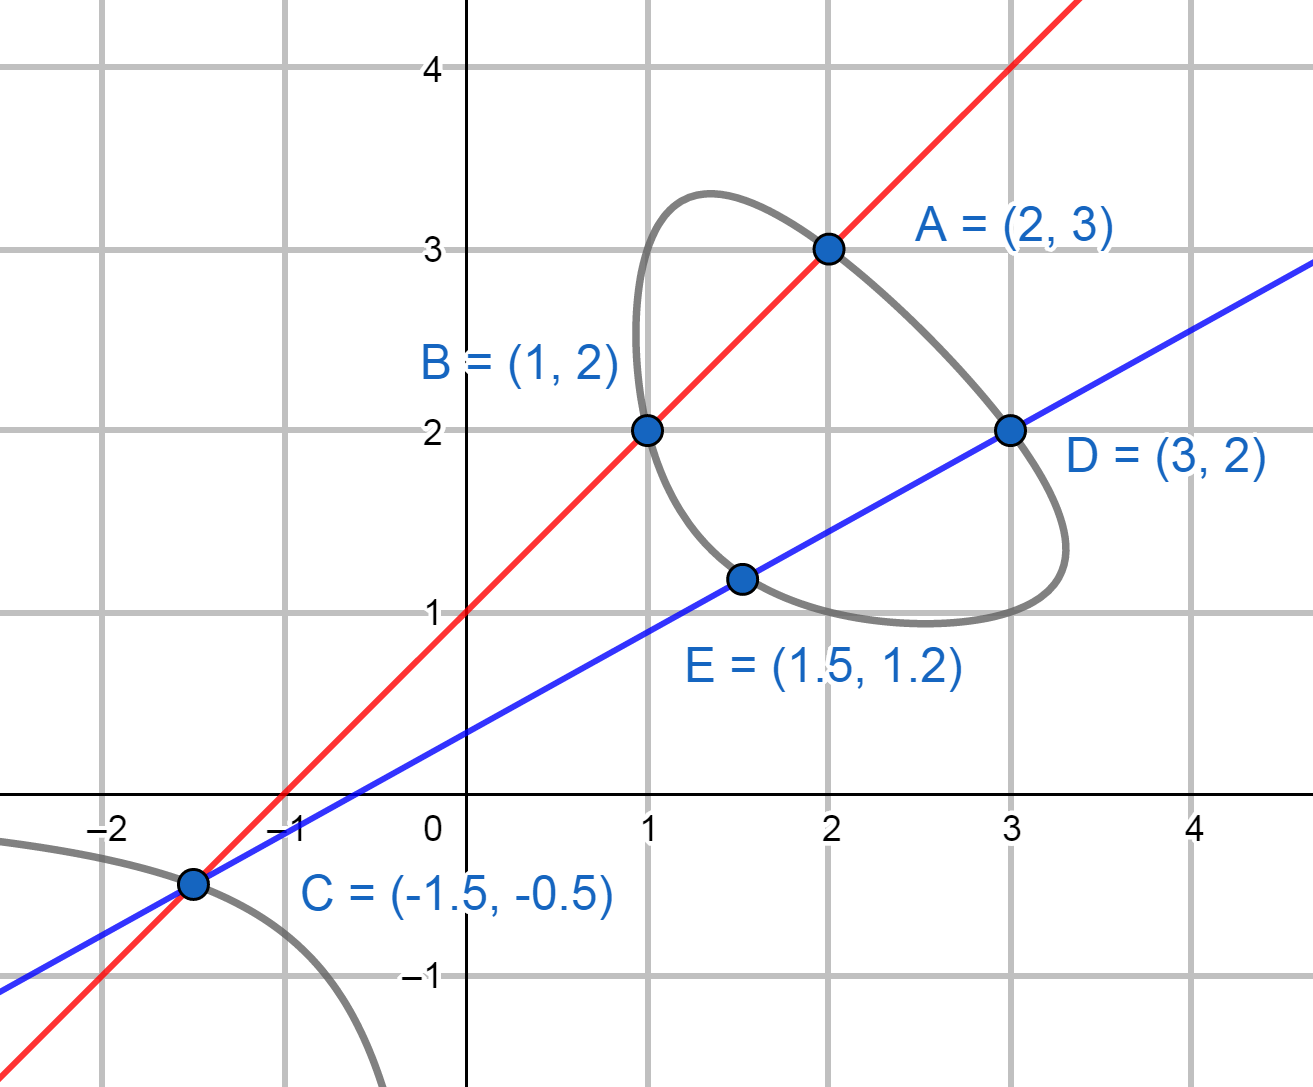
\includegraphics[width=.7\textwidth]{elliptic1}
\end{center}

The equation of the (red) line through $A,B$ is $y=x+1$. Substitute for $y$ in Equation~\ref{eq.elliptic}:
\[
x^2(x+1) + x(x+1)^2 -6x(x+1) +6 =0\,
\]
and simplify:
\[
2x^3 -3x^2 -5x +6 =0\,.
\]
From $A,B$, we know two roots $x=2,x=1$, so we can factor the cubic polynomial as:
\[
(x-2)(x-1)(ax+b)=0\,,
\]
where only the third root is unknown. Multiply the factors and we immediately see that $a$, the coefficient of the cubic term $x^3$, must be $2$, and $2b$, the constant term, must be $6$. Therefore, the third factor is $2x+3$ which gives the third root $x=-\frac{3}{2}$ and $y=x+1=-\disfrac{1}{2}$. This is the point $C=(-\disfrac{3}{2},-\disfrac{1}{2})$ in the graph.

The equation of the second secant (blue) is:
\begin{equation}
y = \frac{5}{9}x + \frac{1}{3}\,.\label{eq.second-secant}
\end{equation}
Substitute for $y$ in Equation~\ref{eq.elliptic}:
\[
x^2\left(\frac{5}{9}x + \frac{1}{3}\right) + x\left(\frac{5}{9}x + \frac{1}{3}\right)^2 -6x\left(\frac{5}{9}x + \frac{1}{3}\right) +6 =0\,,
\]
and simplify:
\[
\frac{70}{81}x^3 - \frac{71}{27}x^2 - \frac{17}{9}x +6 =0\,.
\]
Again, we have two roots $x=3,x=-\disfrac{3}{2}$, so we can factor the cubic polynomial as:
\[
(x-3)\left(x+\frac{3}{2}\right)(ax+b)=0\,.
\]
Equating the coefficient of the cubic term and equating the constant term give:
\[
\frac{70}{81}x - \frac{4}{3}=0\,,
\]
so:
\[
x=\frac{81}{70}\cdot \frac{4}{3}= \frac{27\cdot 4}{70} = \frac{54}{35}\,.
\]
$y$ can be computed from Equation~\ref{eq.second-secant} and the coordinates of $E$ are:
\[
\left(\frac{54}{35}, \frac{25}{21}\right)\,.
\]
Finally, compute $z$ from Equation~\ref{eq.xy1}:
\[
z=\frac{x+y}{xy-1}=%
\displaystyle\left(\frac{54}{35} + \frac{25}{21}\right)%
 \, / \,%
\displaystyle\left(\frac{54}{35}\frac{25}{21}-1\right)=%
\frac{2009}{615} = \frac{49}{15}\,.
\]

\section{From solutions to the elliptic curve to triangles}

From $x,y,z$, $a,b,c$, the sides of the triangle $\triangle ABC$ can be computed:
\begin{eqnarray*}
a&=&w+v = r(z+y)=(z+y)\\
b&=&u+w= r(x+z)=(x+z)\\
c&=&u+v=r(x+y)=(x+y)\,,
\end{eqnarray*}
since $\displaystyle r=\frac{A}{s}=\frac{6}{6}=1$.

For the solution $A=(2,3)$ of the elliptic curve, the value of $z$ is:
\[
z=\frac{x+y}{xy-1}=\frac{2+3}{2\cdot 3-1}=1\,,
\]
and the sides of the triangle are:
\begin{eqnarray*}
a &=& z+y = 1+3 = 4\\
b &=& x+z = 2+1=3\\
c &=& x+y = 2+3=5\,,
\end{eqnarray*}
the right triangle with $s=A=6$. Computing the sides corresponding to $B$ and $D$ gives the same triangle.

For $E$:
\begin{eqnarray*}
a &=& z+y = \frac{49}{15} + \frac{25}{21} = \frac{156}{35}\\
b &=& x+z = \frac{54}{35} + \frac{49}{15} = \frac{101}{21}\\
c &=& x+y = \frac{54}{35} + \frac{25}{21}  = \frac{41}{15}\,.
\end{eqnarray*}

Let us check the result. The semi-perimeter is:
\[
s=\frac{1}{2}\left(\frac{156}{35} + \frac{101}{21}+\frac{41}{15}\right) = \frac{1}{2}\left(\frac{468+505+287}{105}\right) = \frac{1}{2}\left(\frac{1260}{105}\right)= 6\,,
\]
and the area can be computed using Heron's formula:
\begin{eqnarray*}
A &=& \sqrt{s(s-a)(s-b)(s-c)}\\
&=& \sqrt{6 \left(6-\frac{156}{35}\right) \left(6-\frac{101}{21}\right) \left(6-\frac{41}{15}\right)}\\
&=& \sqrt{6 \cdot \frac{54}{35}\cdot \frac{25}{21} \cdot \frac{49}{15}}\\
&=& \sqrt{\frac{396900}{11025}}\\
&=& \sqrt{36} = 6\,.
\end{eqnarray*}

\section{A proof of Heron's formula}

The triple tangent formula states that if $\phi+\theta+\psi=\pi$ then:
\begin{equation}
\tan\phi+\tan\theta+\tan\psi = \tan\phi\tan\theta\tan\psi\,. \label{eq.triple}
\end{equation}
The proof follows immediately from Equation~\ref{eq.tangent3}:
\begin{eqnarray*}
\tan\psi &=& \tan (\pi-(\phi+\theta))\\
&=& -\tan (\phi+\theta)\\
&=& \frac{\tan\phi+\tan\theta}{\tan\phi\tan\theta-1}\\
\tan\phi\tan\theta\tan\psi-\tan\psi&=& \tan\phi+\tan\theta\\
\tan\phi\tan\theta\tan\psi &=&\tan\phi+\tan\theta+\tan\psi\,.
\end{eqnarray*}
From Equations~\ref{eq.alpha}--\ref{eq.area2}, and $r=A/s$:
\begin{eqnarray*}
A &=& r^2\left(\tan \frac{\alpha}{2}+\tan \frac{\beta}{2}+\tan \frac{\gamma}{2}\right)\\
&=&r^2\left(\tan \frac{\alpha}{2}\tan \frac{\beta}{2}\tan \frac{\gamma}{2}\right)\\
&=&r^2\left(\frac{u}{r}\frac{v}{r}\frac{w}{r}\right)\\
&=&\frac{u\,v\,w}{r}\\
&=&\frac{s}{A}\,u\,v\,w\\
A^2&=&s\,u\,v\,w\,.
\end{eqnarray*}
$s=u+v+w$, so:
\begin{eqnarray*}
s - a &=& (u+v+w) - (w+v) = u\\
s - b &=& (u+v+w) - (u+w) = v\\
s - c &=& (u+v+w) - (u+v) = w\,,
\end{eqnarray*}
and Heron's formula follows:
\begin{eqnarray*}
A^2 &=& s\,u\,v\,w\\
&=& s(s-a)(s-b)(s-c)\\
A &=& \sqrt{s(s-a)(s-b)(s-c)}\,.
\end{eqnarray*}




% !TeX root = origami-activities-en.tex

%%%%%%%%%%%%%%%%%%%%%%%%%%%%%%%%%%%%%%%%%%%%%%%%%%%%%%%%%%%%%%%%%%
%%%%%%%%%%%%%%%%%%%%%%%%%%%%%%%%%%%%%%%%%%%%%%%%%%%%%%%%%%%%%%%%%%
%%%%%%%%%%%%%%%%%%%%%%%%%%%%%%%%%%%%%%%%%%%%%%%%%%%%%%%%%%%%%%%%%%

\section*{Further reading}

Applications of origami \cite{lang-ted}. Mathematical theory of origami \cite{alperin,moti-origami}. History of origami \cite{history}. Paper folding \cite{lang,newton}.


\bibliographystyle{plain}
\bibliography{origami-activities-en}


\end{document}
